\documentclass[11pt]{article}

\usepackage[utf8]{inputenc}
\usepackage[T1]{fontenc}
\usepackage{geometry}
\usepackage{graphicx}
\usepackage{booktabs}
\usepackage{float}
\usepackage{hyperref}

\geometry{letterpaper, margin=2.2cm}
\graphicspath{{figures/}}

\title{Motor 2: calibracion de respuesta antes de ajustar reward}
\author{Proyecto Protesis Mioelectrica TD3}
\date{2026-06-23}

\begin{document}
\maketitle

\section{Resumen}

Se reviso una fase corta de diagnostico para motor 2 antes de volver a
entrenar campanas largas o retomar Residual Lift y stop-band. El objetivo
fue separar donde aparece el bajo flujo util del motor 2: en el simulador
de encoder, en \texttt{encoder2Flex}, o en \texttt{flexJoined\_scale}.

El trabajo siguio siendo solo software/simulacion. No se activo hardware,
no se cambiaron puertos COM y no se promovio ninguna configuracion nueva
como default.

\section{Por que se hizo}

La fase anterior mostro que la reward ponderada en motor 2 redujo
\texttt{trackingMSE\_motor2}, pero no aumento \texttt{responseRange\_motor2}
ni redujo de forma robusta los flags \texttt{motor2\_flat\_response} y
\texttt{motor2\_action\_no\_motion}. Por eso se aislo primero la respuesta
del simulador y la conversion encoder-flex.

La pregunta principal fue directa: si el encoder se mueve pero el flex
normalizado no cambia, entonces el problema no esta solamente en la accion
del agente.

\section{Diagnostico encoder a flex}

Se ejecuto:

\begin{verbatim}
results = run_motor_response_conversion_diagnostic();
\end{verbatim}

La prueba aplico niveles \texttt{[-1 -0.75 -0.50 -0.25 0 0.25 0.50 0.75 1]}
por motor. En motor 2 se observo que niveles bajos si mueven encoder, pero
no producen flex util hasta cruzar la zona efectiva de \texttt{encoder2Flex}.

\begin{table}[H]
\centering
\caption{Motor 2: conversion encoder-flex desde home.}
\begin{tabular}{rrrrrl}
\toprule
Accion & PWM & Encoder range & encoder2Flex & Flex norm & Etapa \\
\midrule
-1.00 & -255 & 437.333 & 0.000 & 0.000 & encoder2Flex flat \\
-0.25 & -64 & 15.000 & 0.000 & 0.000 & encoder2Flex flat \\
0.25 & 64 & 3598.000 & 0.000 & 0.000 & encoder2Flex flat \\
0.50 & 128 & 6113.833 & 359.688 & 0.175801 & responsive \\
1.00 & 255 & 6665.167 & 440.176 & 0.215140 & responsive \\
\bottomrule
\end{tabular}
\end{table}

La lectura es que el aplanamiento bajo no ocurre en el encoder del
simulador. Ocurre despues, en la conversion \texttt{encoder2Flex}, por la
zona de gap/limites. En motor 2, una accion de \texttt{0.25} mueve el
encoder \texttt{3598}, pero deja \texttt{encoder2FlexRange=0}.

\begin{figure}[H]
\centering
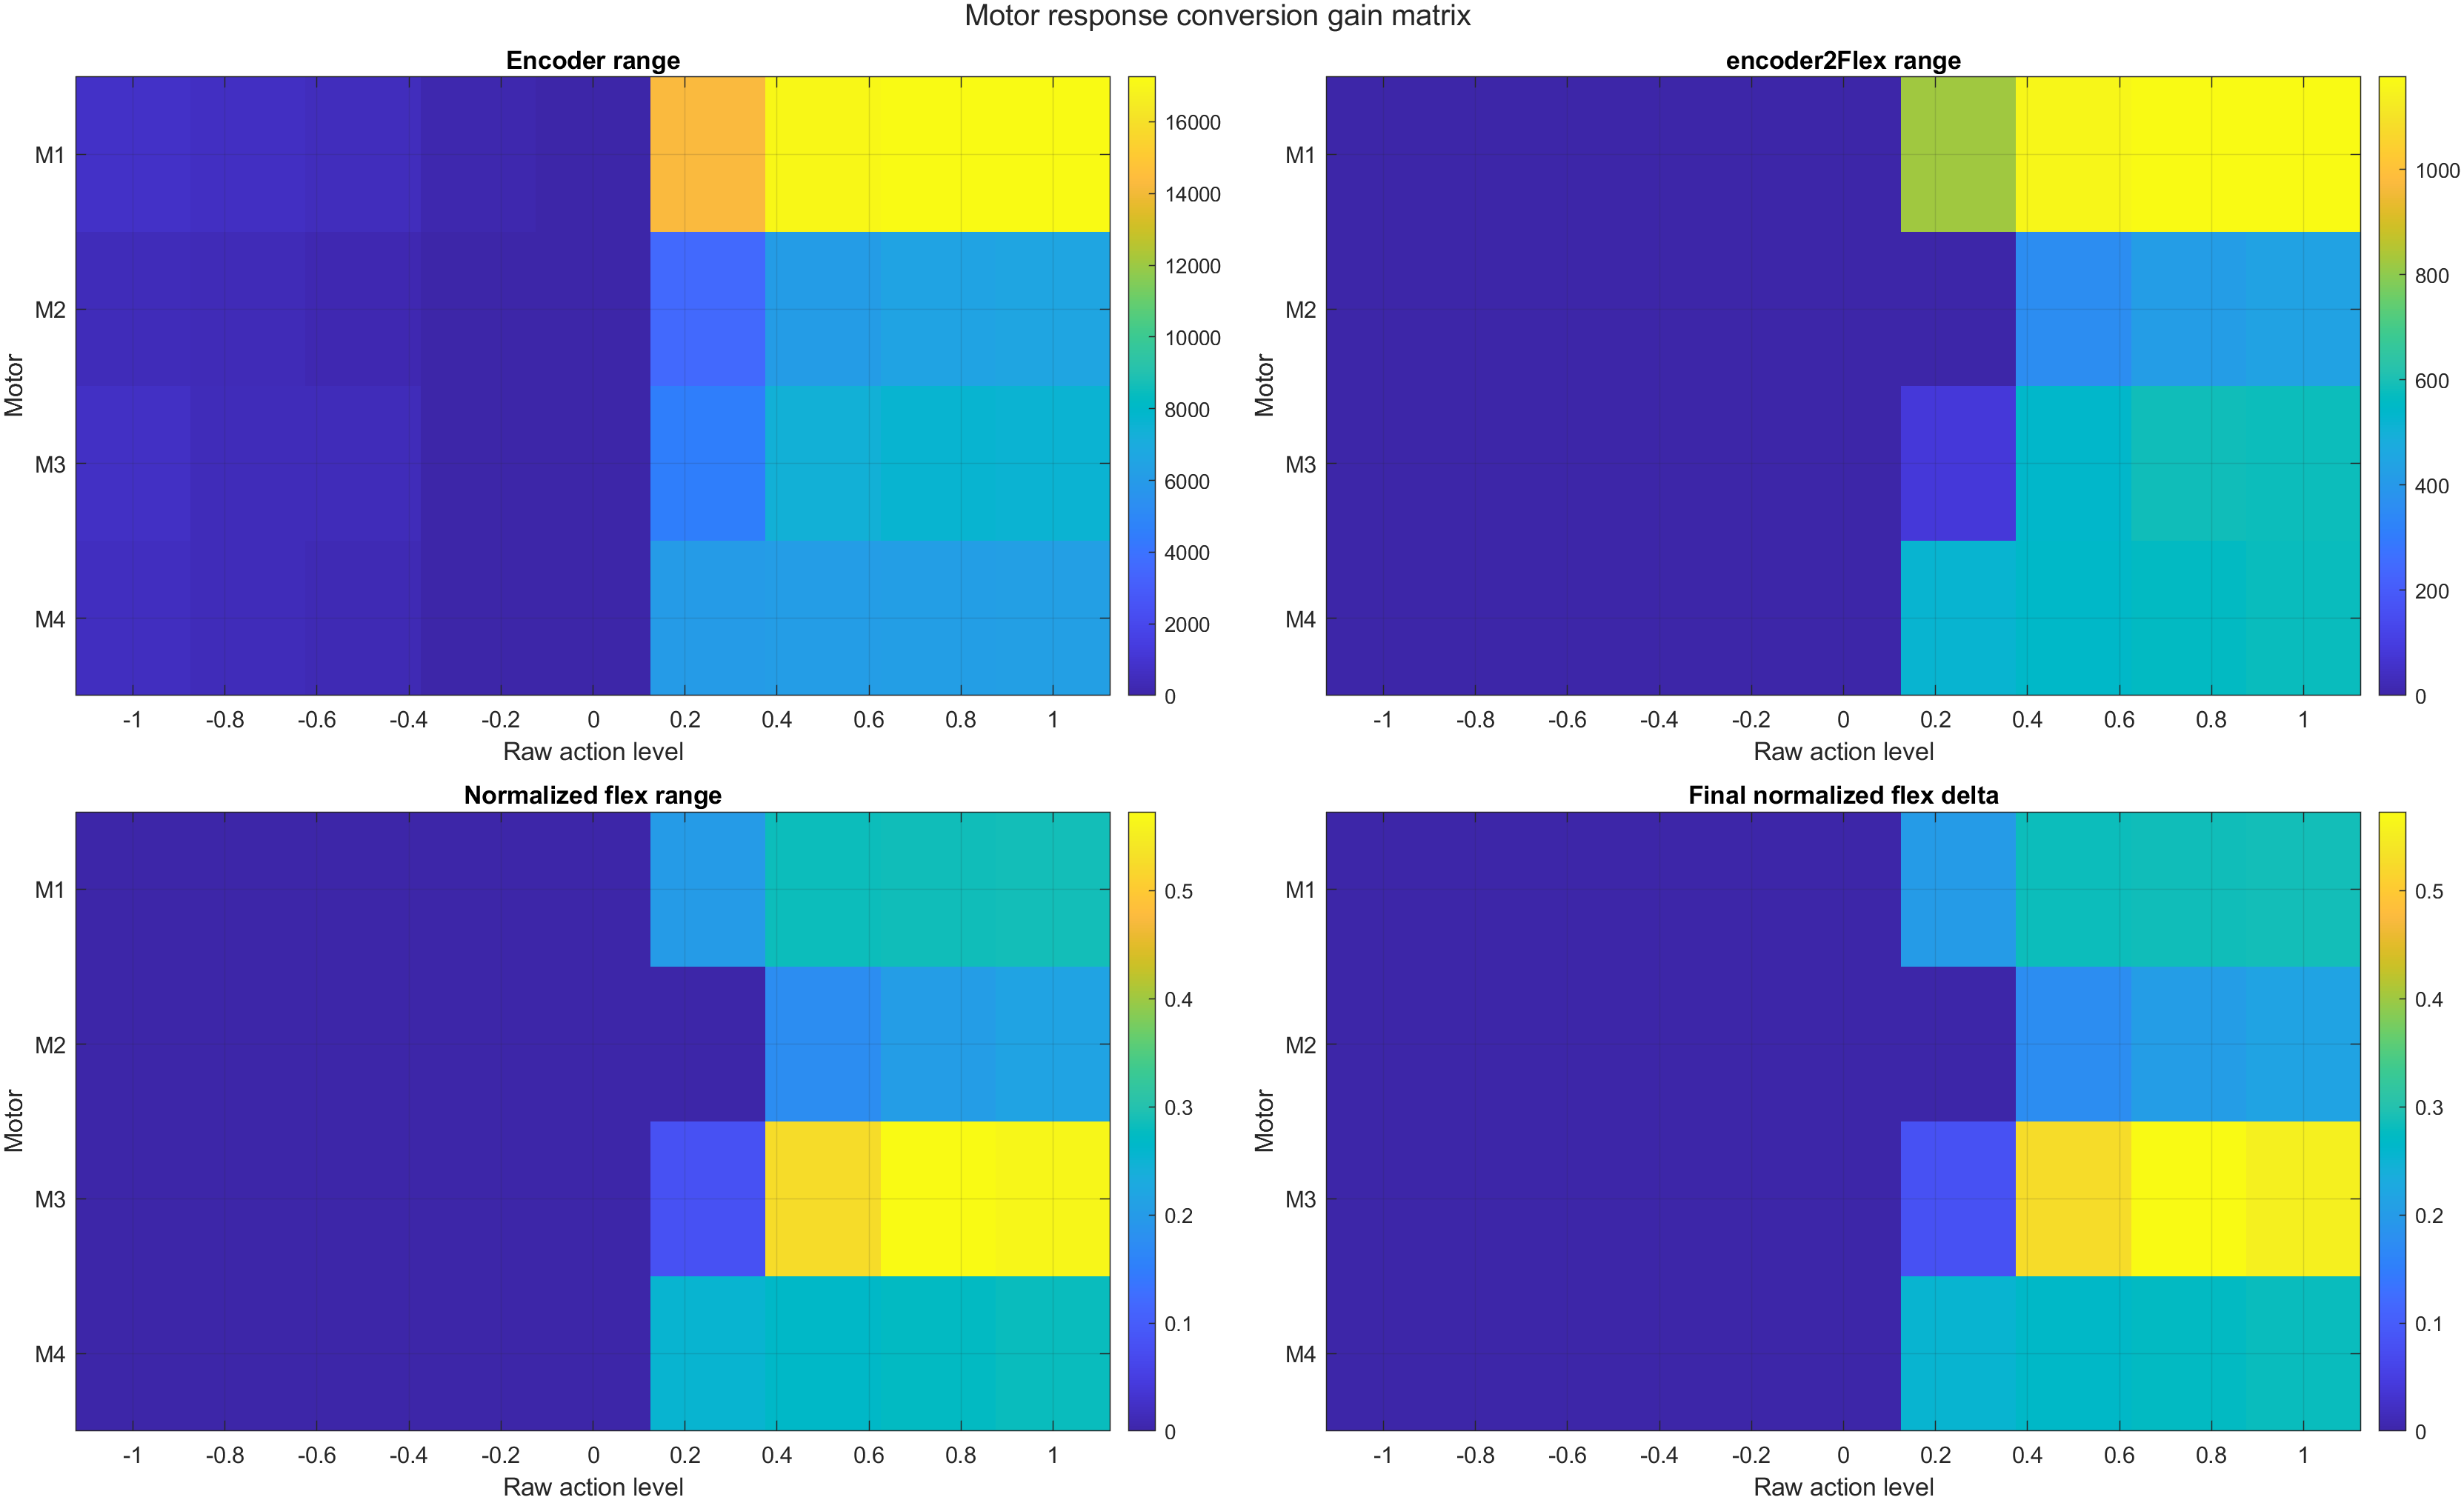
\includegraphics[width=0.92\linewidth]{calibration_motor_response_conversion_gain_matrix.png}
\caption{Matriz MATLAB de rangos encoder, encoder2Flex y flex normalizado.}
\end{figure}

\section{Sanity con posiciones iniciales}

Se ejecuto:

\begin{verbatim}
results = run_motor2_simulation_sanity_check_extended(struct( ...
    'initialMode','all'));
\end{verbatim}

El objetivo fue no concluir que la accion negativa falla cuando la posicion
inicial ya esta abierta. Se probaron tres modos: \texttt{home},
\texttt{mid} y \texttt{closed}.

\begin{table}[H]
\centering
\caption{Motor 2: rango flex promedio por modo inicial.}
\begin{tabular}{lrr}
\toprule
Modo inicial & Positive mean range flex & Negative mean range flex \\
\midrule
home & 0.148948 & 0.000000 \\
mid & 0.131110 & 0.280059 \\
closed & 0.411169 & 0.560117 \\
\bottomrule
\end{tabular}
\end{table}

La accion negativa desde \texttt{home} no fue concluyente. Desde
\texttt{mid} y \texttt{closed}, motor 2 si mostro rango flex util con
acciones negativas. Esto indica que la asimetria observada depende mucho de
la posicion inicial y de la zona util de conversion.

\begin{figure}[H]
\centering
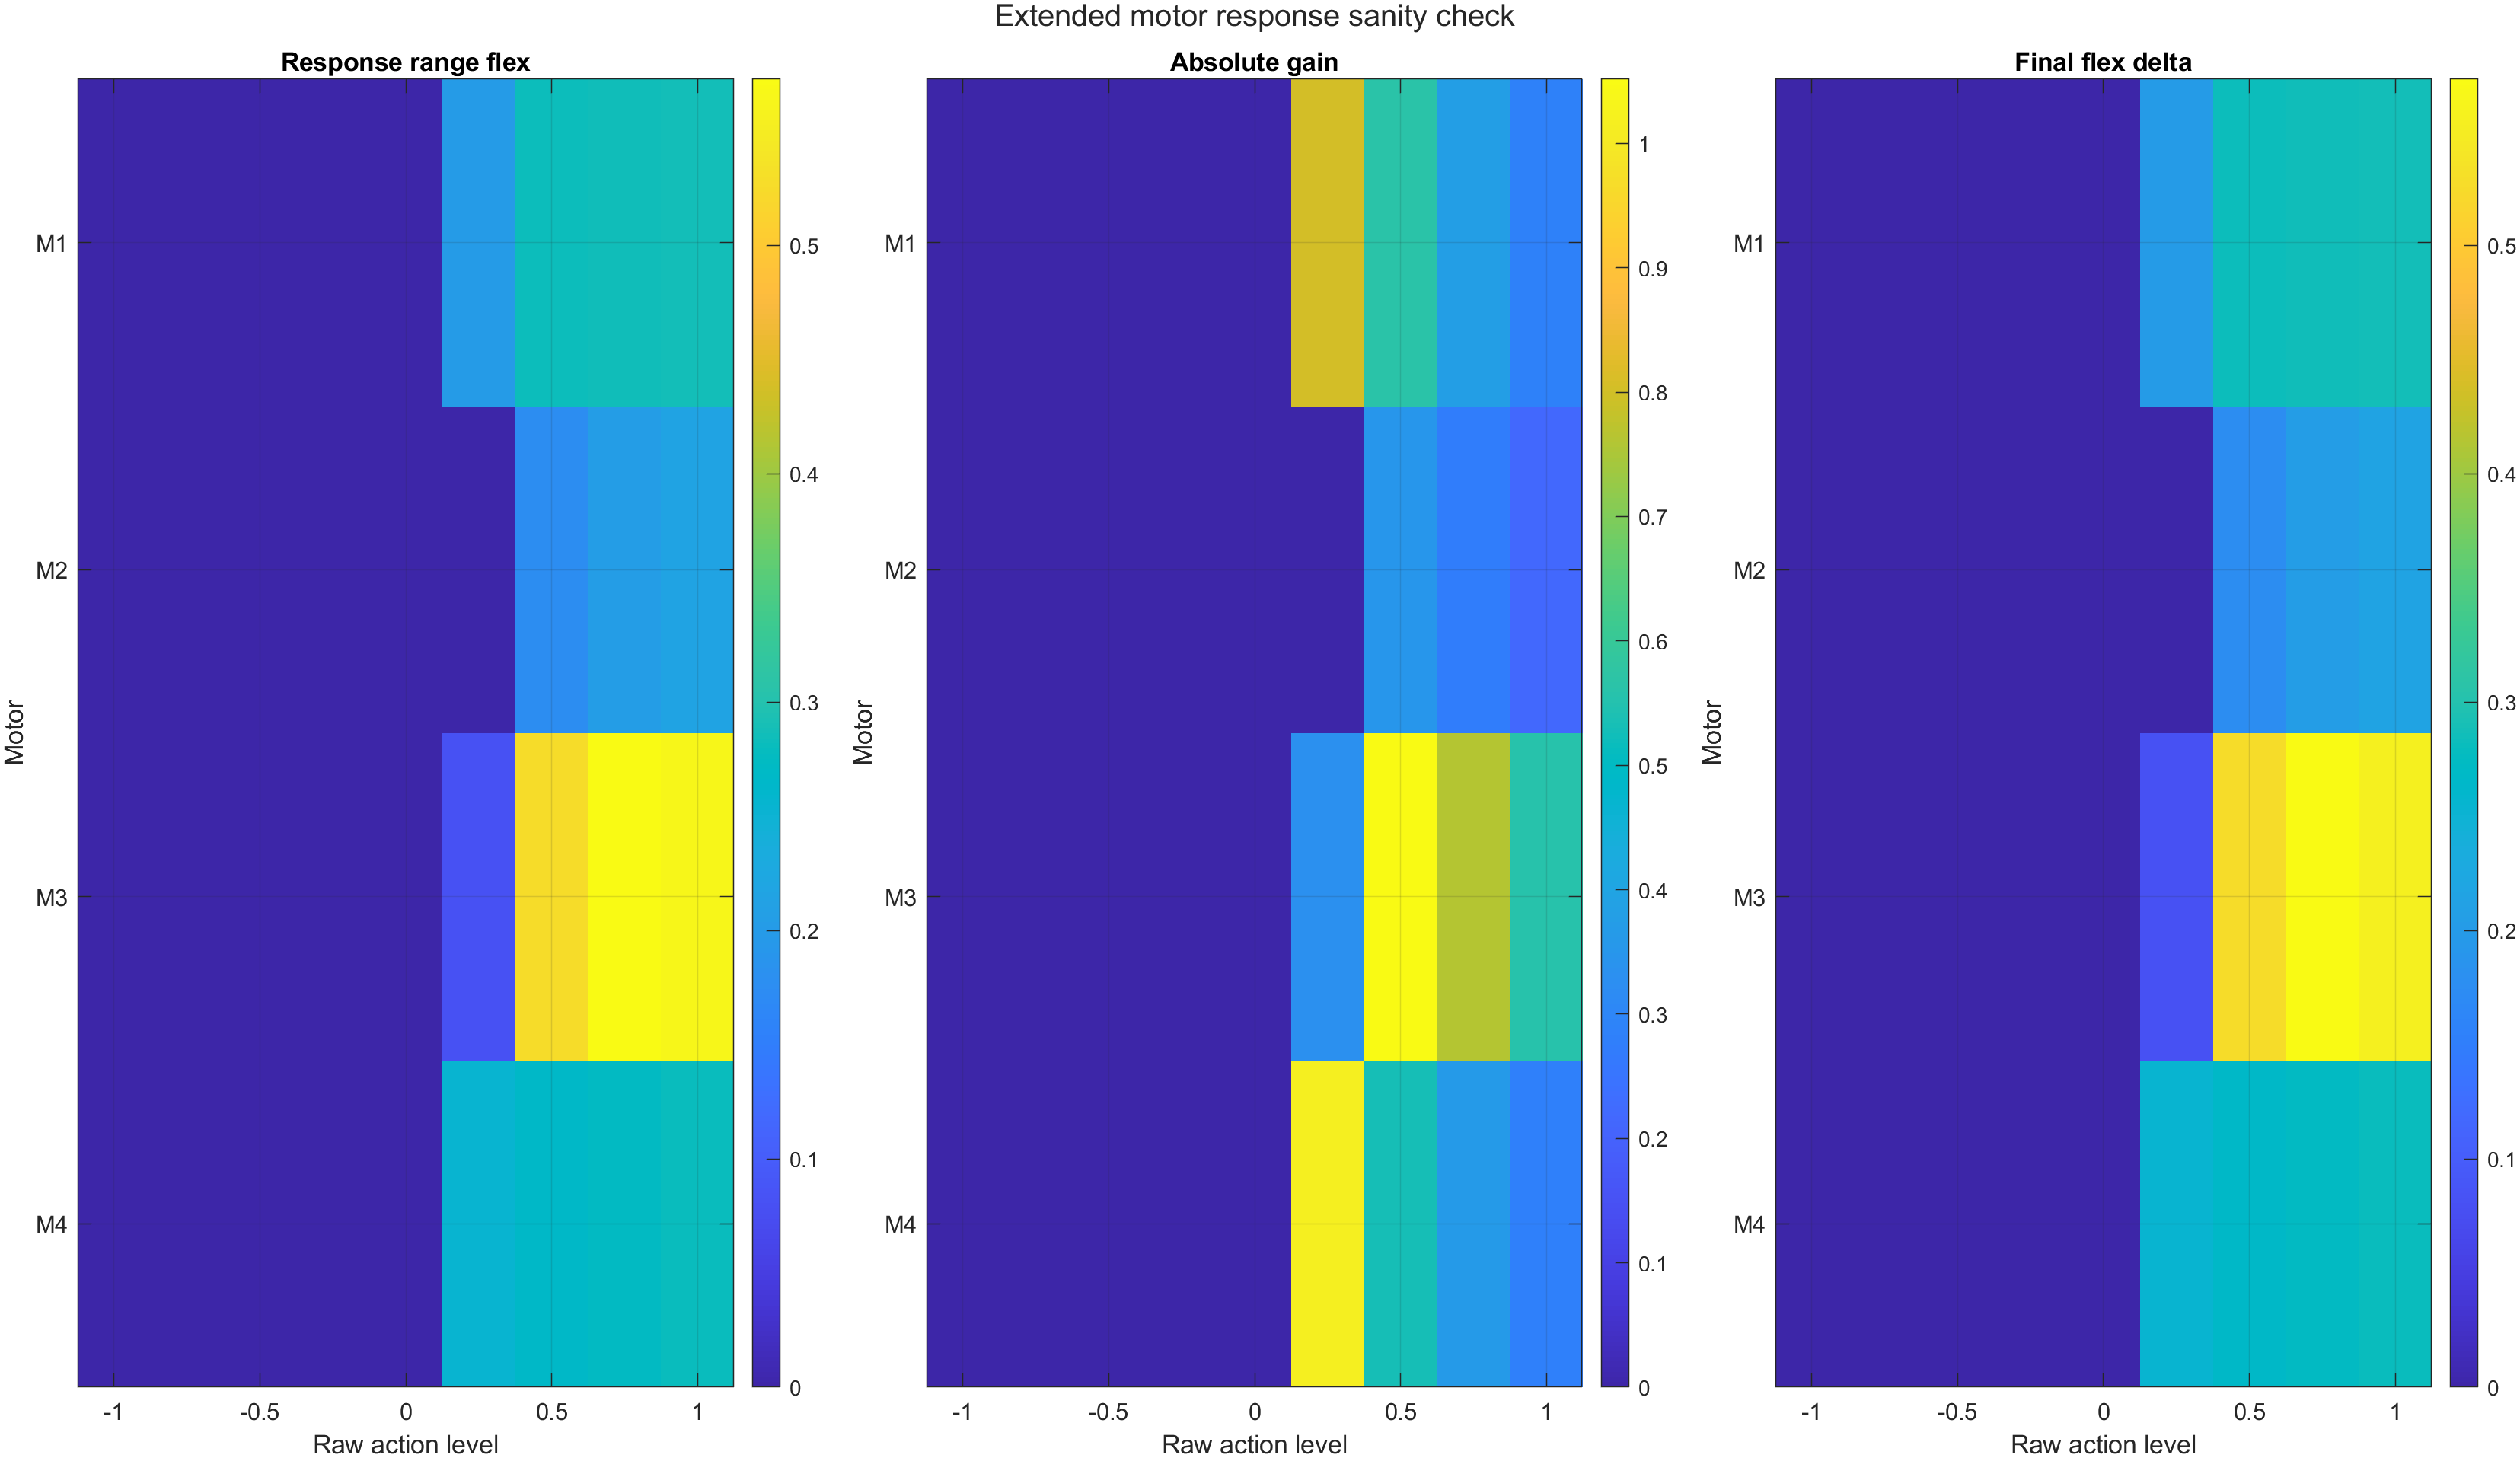
\includegraphics[width=0.92\linewidth]{calibration_sanity_home.png}
\caption{Sanity MATLAB desde home.}
\end{figure}

\begin{figure}[H]
\centering
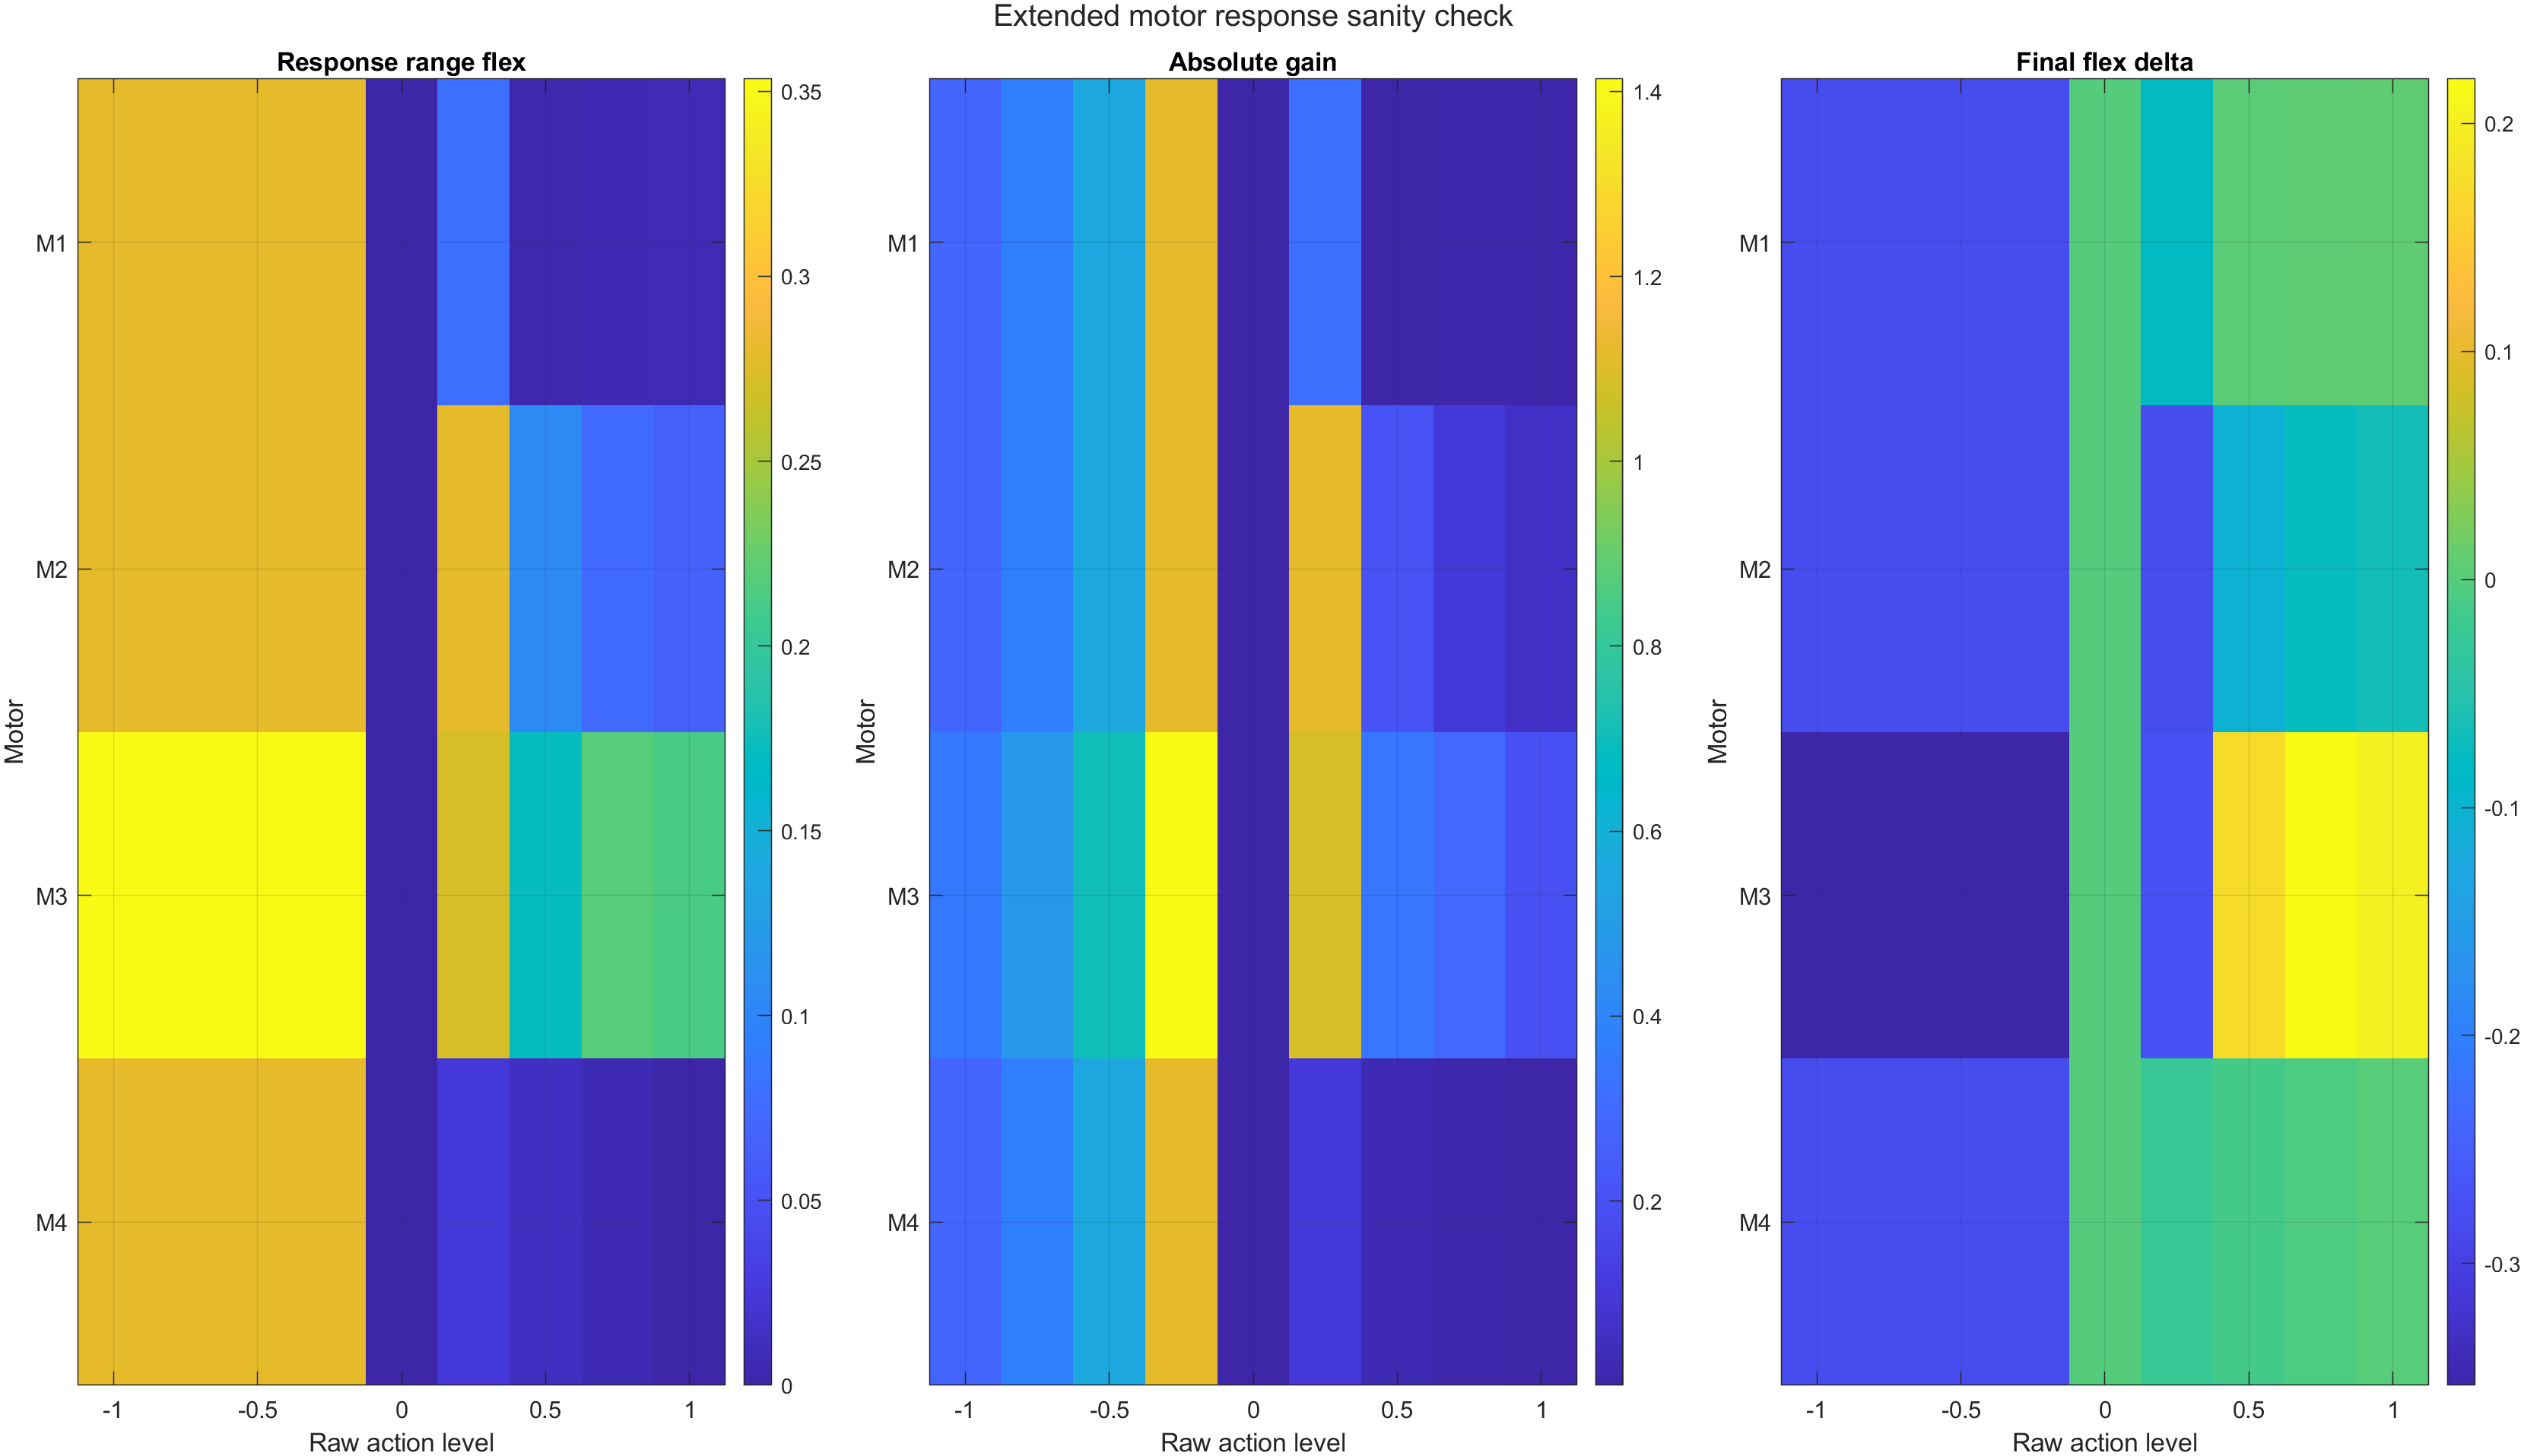
\includegraphics[width=0.92\linewidth]{calibration_sanity_mid.png}
\caption{Sanity MATLAB desde posicion media.}
\end{figure}

\section{Ablation de accion calibrada}

Se ejecuto una prueba corta:

\begin{verbatim}
results = run_motor2_calibrated_action_ablation(struct( ...
    'seeds', [11 55], ...
    'trainingEpisodes', 500, ...
    'finalTestEpisodes', 5, ...
    'useGpu', true));
\end{verbatim}

Se compararon tres configuraciones: baseline cuantizado, accion continua y
\texttt{motorCalibratedQuantized}. La calibrada uso niveles mas altos para
motor 2 en simulacion, sin cambiar el default oficial.

\begin{table}[H]
\centering
\caption{Ablation corta, promedio de seeds 11 y 55.}
\begin{tabular}{lrrrrrr}
\toprule
Config & MSE & MAE & MSE M2 & Range M2 & Saturacion & Flags M2 \\
\midrule
baseline & 0.099748 & 0.257544 & 0.112913 & 0.170200 & 0.169857 & 1 flat, 0 no-motion \\
continua & 0.095778 & 0.254492 & 0.089930 & 0.138397 & 0.145979 & 1 flat, 0 no-motion \\
calibrada & 0.092527 & 0.252928 & 0.070589 & 0.167690 & 0.053934 & 1 flat, 1 no-motion \\
\bottomrule
\end{tabular}
\end{table}

La accion calibrada mejoro el error global, bajo el error de motor 2 y
redujo bastante la saturacion. Sin embargo, no aumento el rango util
promedio de motor 2 frente al baseline y dejo un flag
\texttt{motor2\_action\_no\_motion}. Por eso no paso el criterio de
aceptacion.

\begin{figure}[H]
\centering
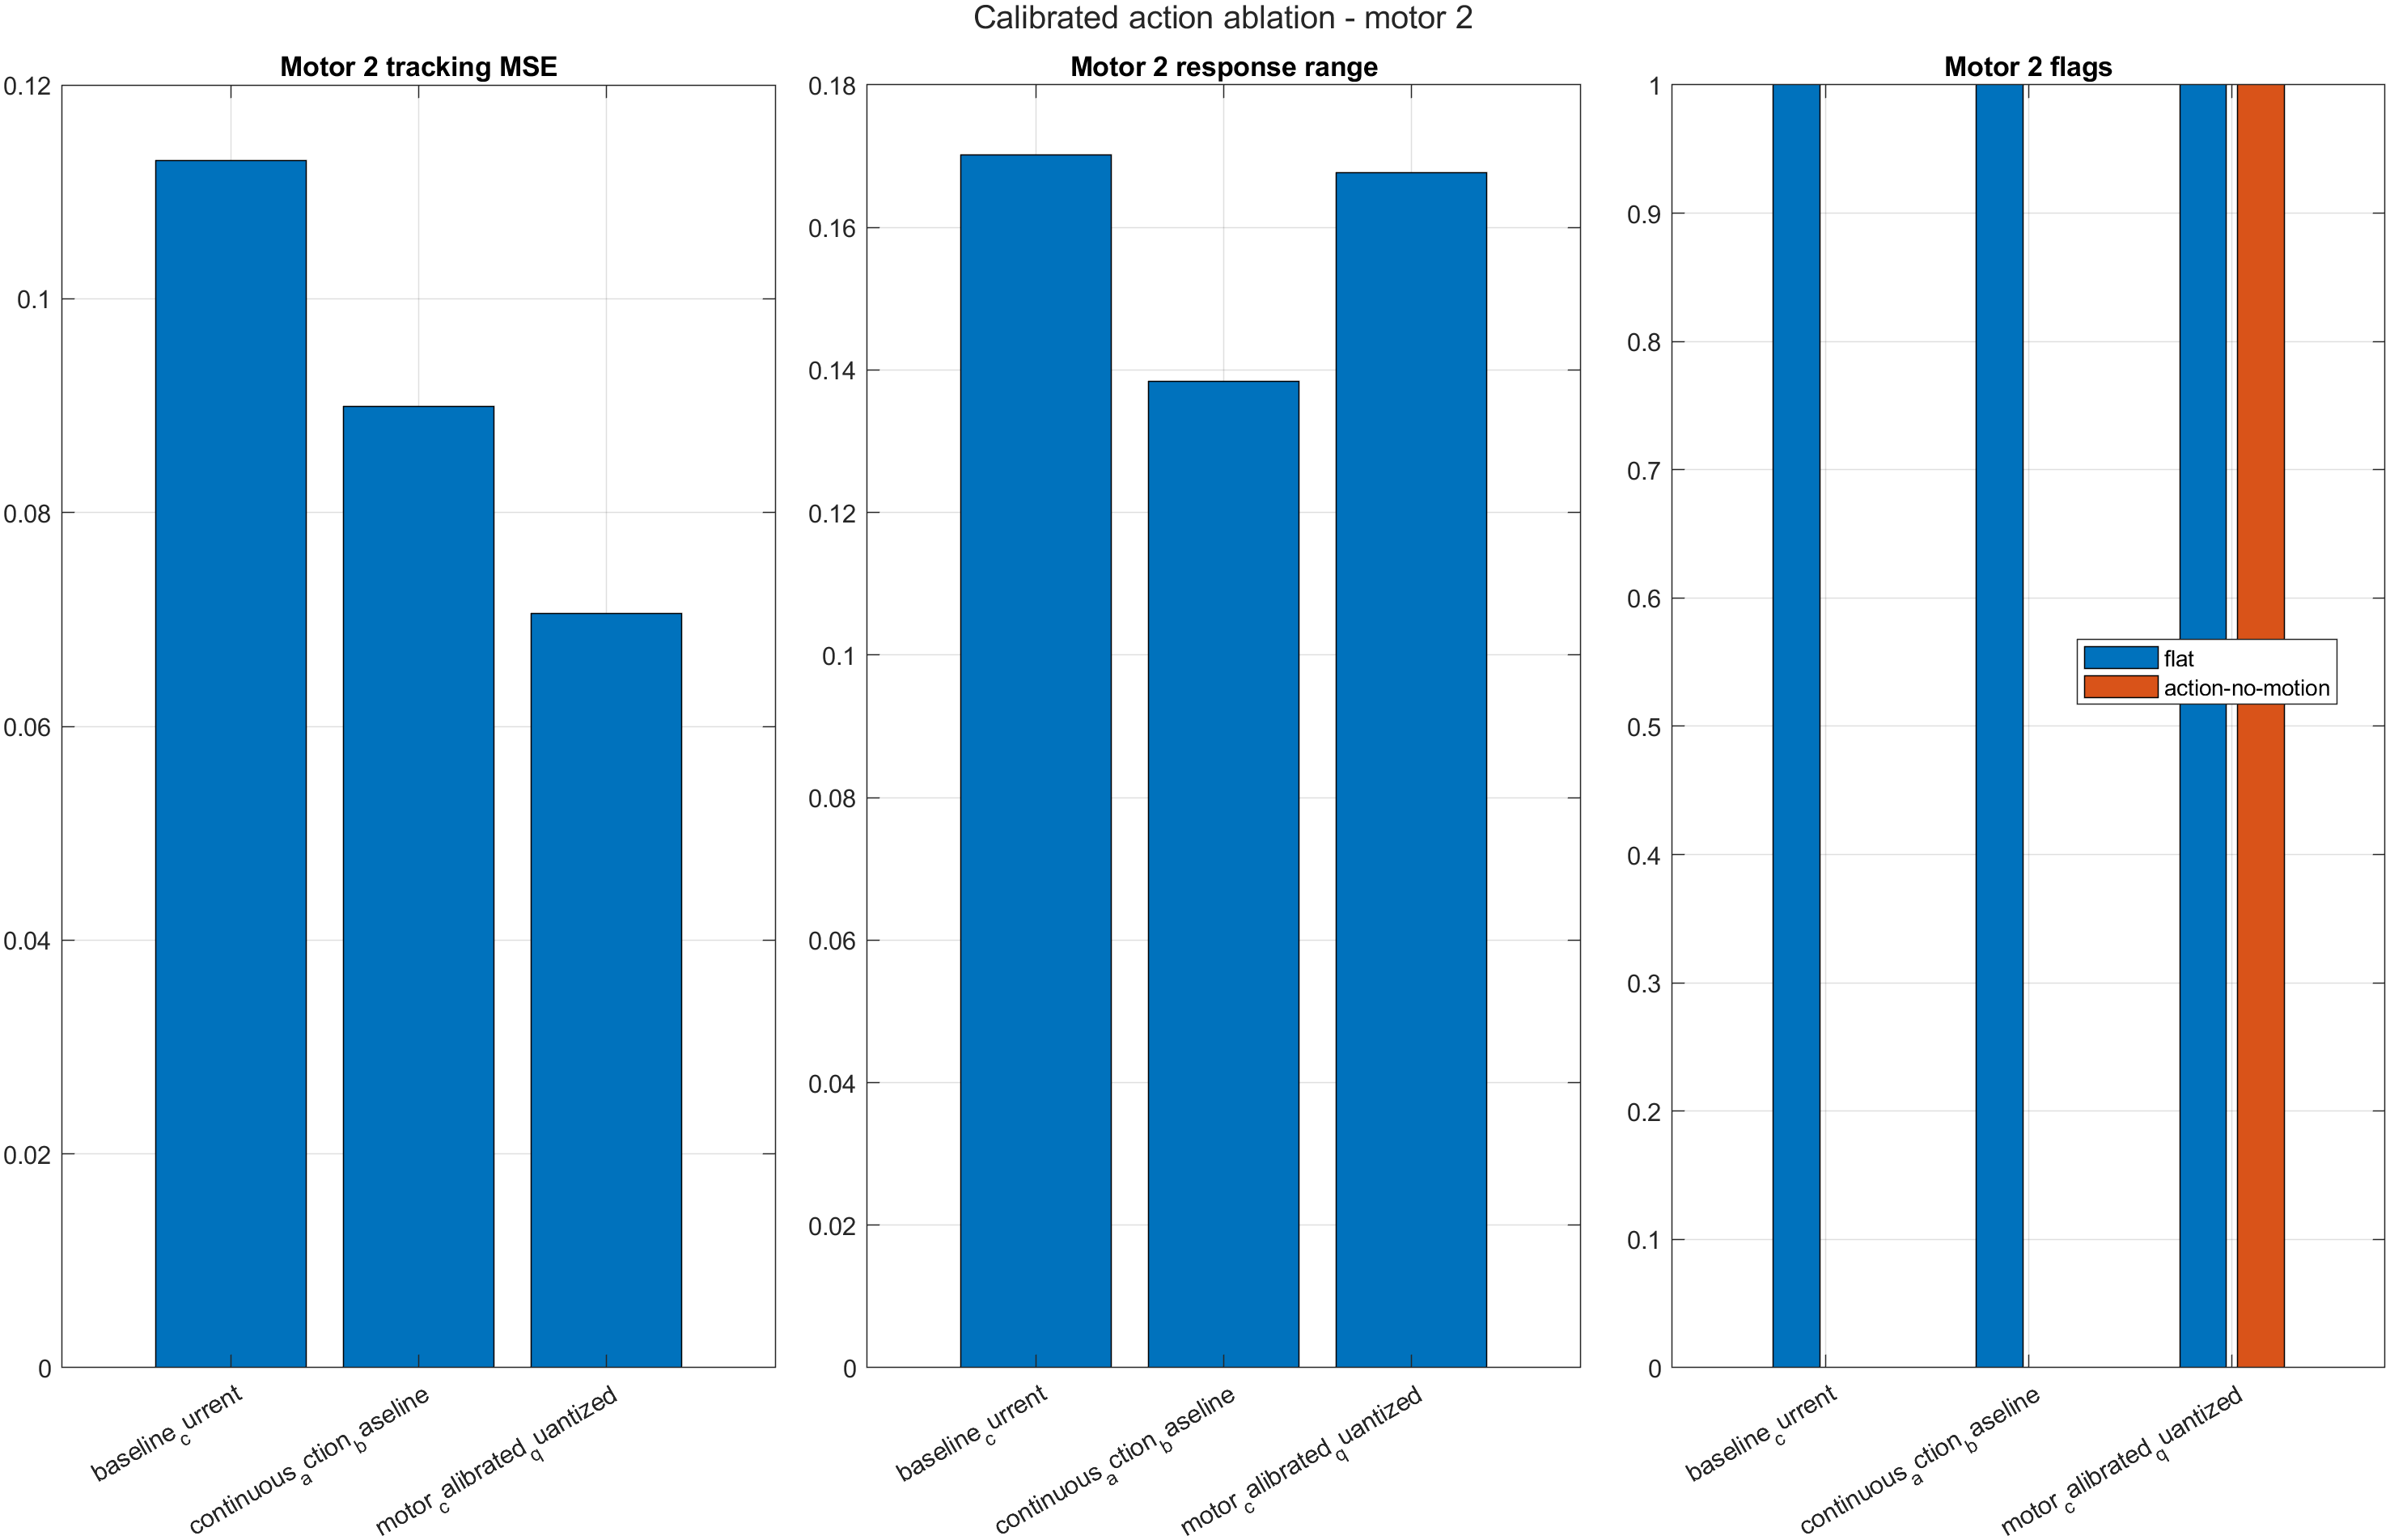
\includegraphics[width=0.92\linewidth]{calibration_ablation_motor2.png}
\caption{Resumen MATLAB de motor 2 en la ablation calibrada.}
\end{figure}

\begin{figure}[H]
\centering
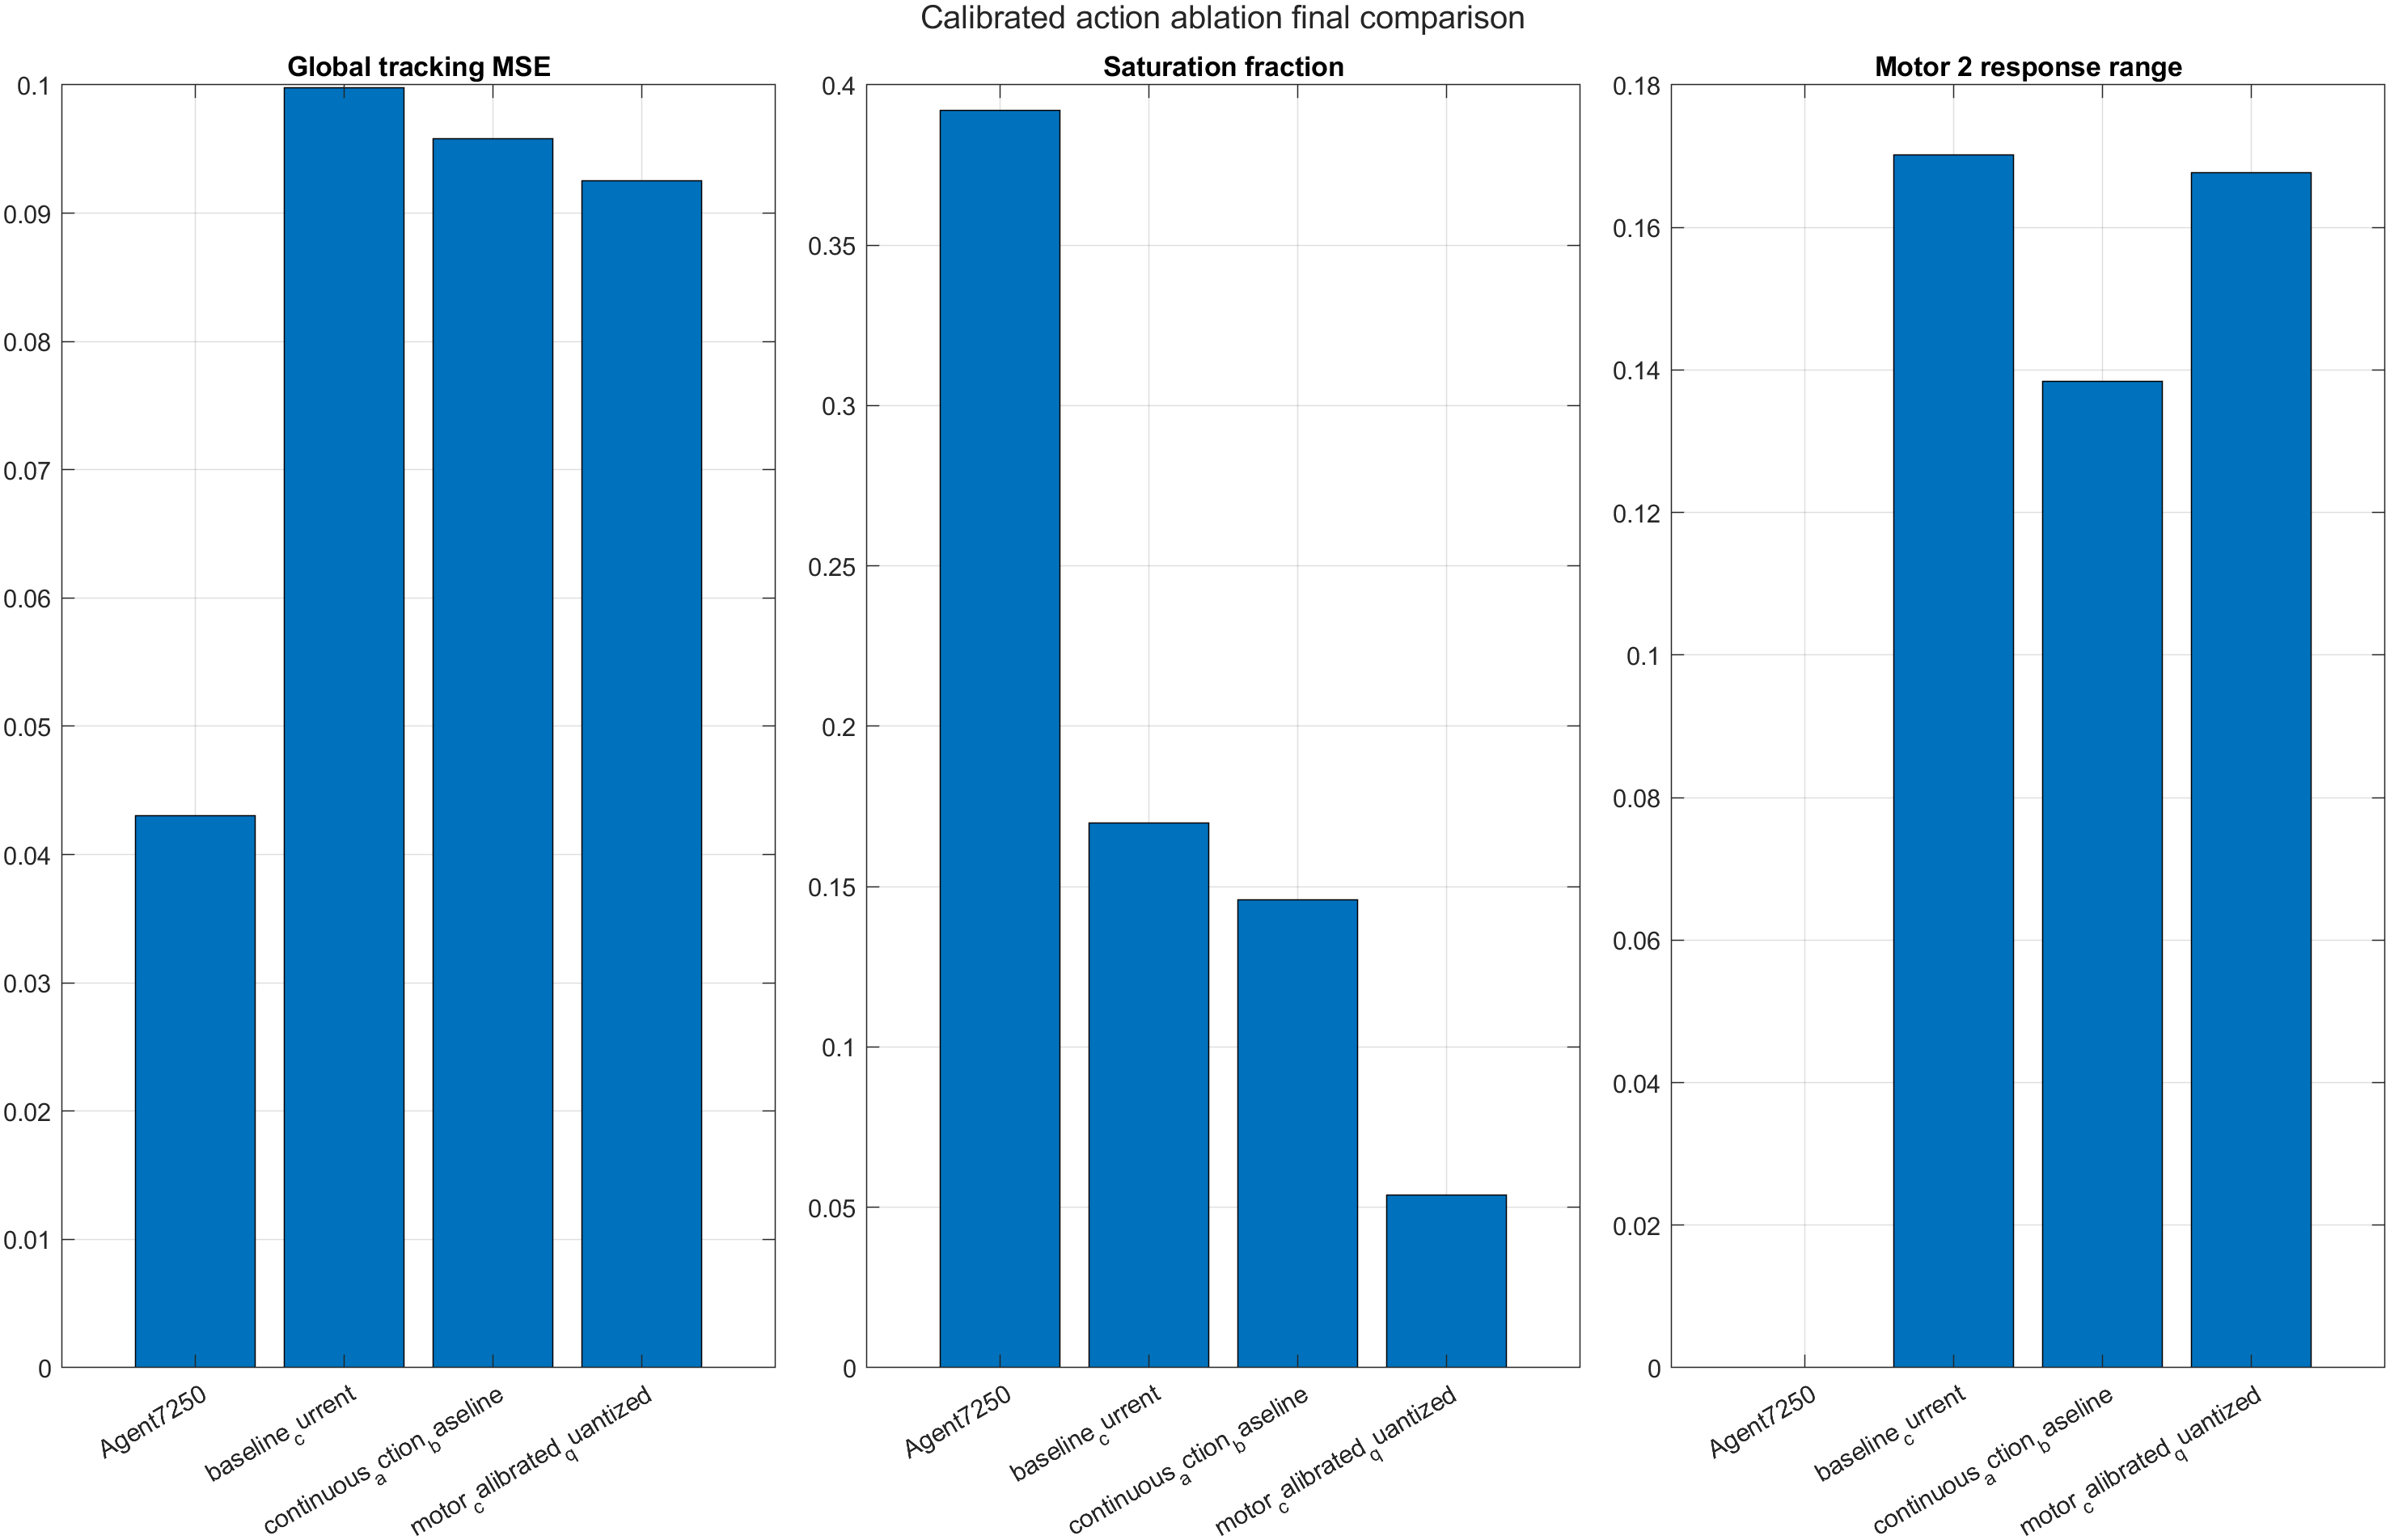
\includegraphics[width=0.92\linewidth]{calibration_ablation_final_comparison.png}
\caption{Comparacion final MATLAB de la ablation calibrada.}
\end{figure}

\section{Intento de conversion encoder2Flex}

Despues se probo una correccion experimental en \texttt{encoder2Flex} para
motor 2. No se cambio el default oficial. La prueba aceptada uso
\texttt{baselineQuantized}, \texttt{encoder2FlexVariant="motor2Calibrated"}
y \texttt{motor2Encoder2FlexGapOffset=-256}. La seleccion final uso
\texttt{selectionMode="motor2\_final\_gate"} para probar varios checkpoints
antes de aceptar una seed.

La corrida corta quedo en:

\begin{verbatim}
Agentes/motor2_conversion_fix_ablation/26-06-18_02-49-24/
\end{verbatim}

\begin{table}[H]
\centering
\caption{Ablation de conversion, seeds 11 y 55, 500 episodios.}
\begin{tabular}{lrrrrrrr}
\toprule
Config & MSE & MSE M2 & Range M2 & Saturacion & Flat & No-motion & Aceptada \\
\midrule
baseline + baseline & 0.099748 & 0.112913 & 0.170200 & 0.169857 & 1 & 0 & no \\
baseline + motor2Cal & 0.092616 & 0.078885 & 0.181432 & 0.133639 & 0 & 0 & si \\
accion cal + baseline & 0.092527 & 0.070589 & 0.167690 & 0.053934 & 1 & 1 & no \\
accion cal + motor2Cal & 0.075777 & 0.078055 & 0.172212 & 0.108406 & 1 & 1 & no \\
\bottomrule
\end{tabular}
\end{table}

La configuracion \texttt{baselineQuantized + motor2Calibrated} paso el smoke
centrado en motor 2. Frente al baseline, bajo el MSE global, bajo el MSE de
motor 2, subio \texttt{responseRange\_motor2} y dejo los flags de motor 2 en
cero para ese smoke. La aceptacion quedo revocada por la validacion
all-motor posterior. La accion calibrada no se promovio porque siguio dejando
flags.

\begin{figure}[H]
\centering
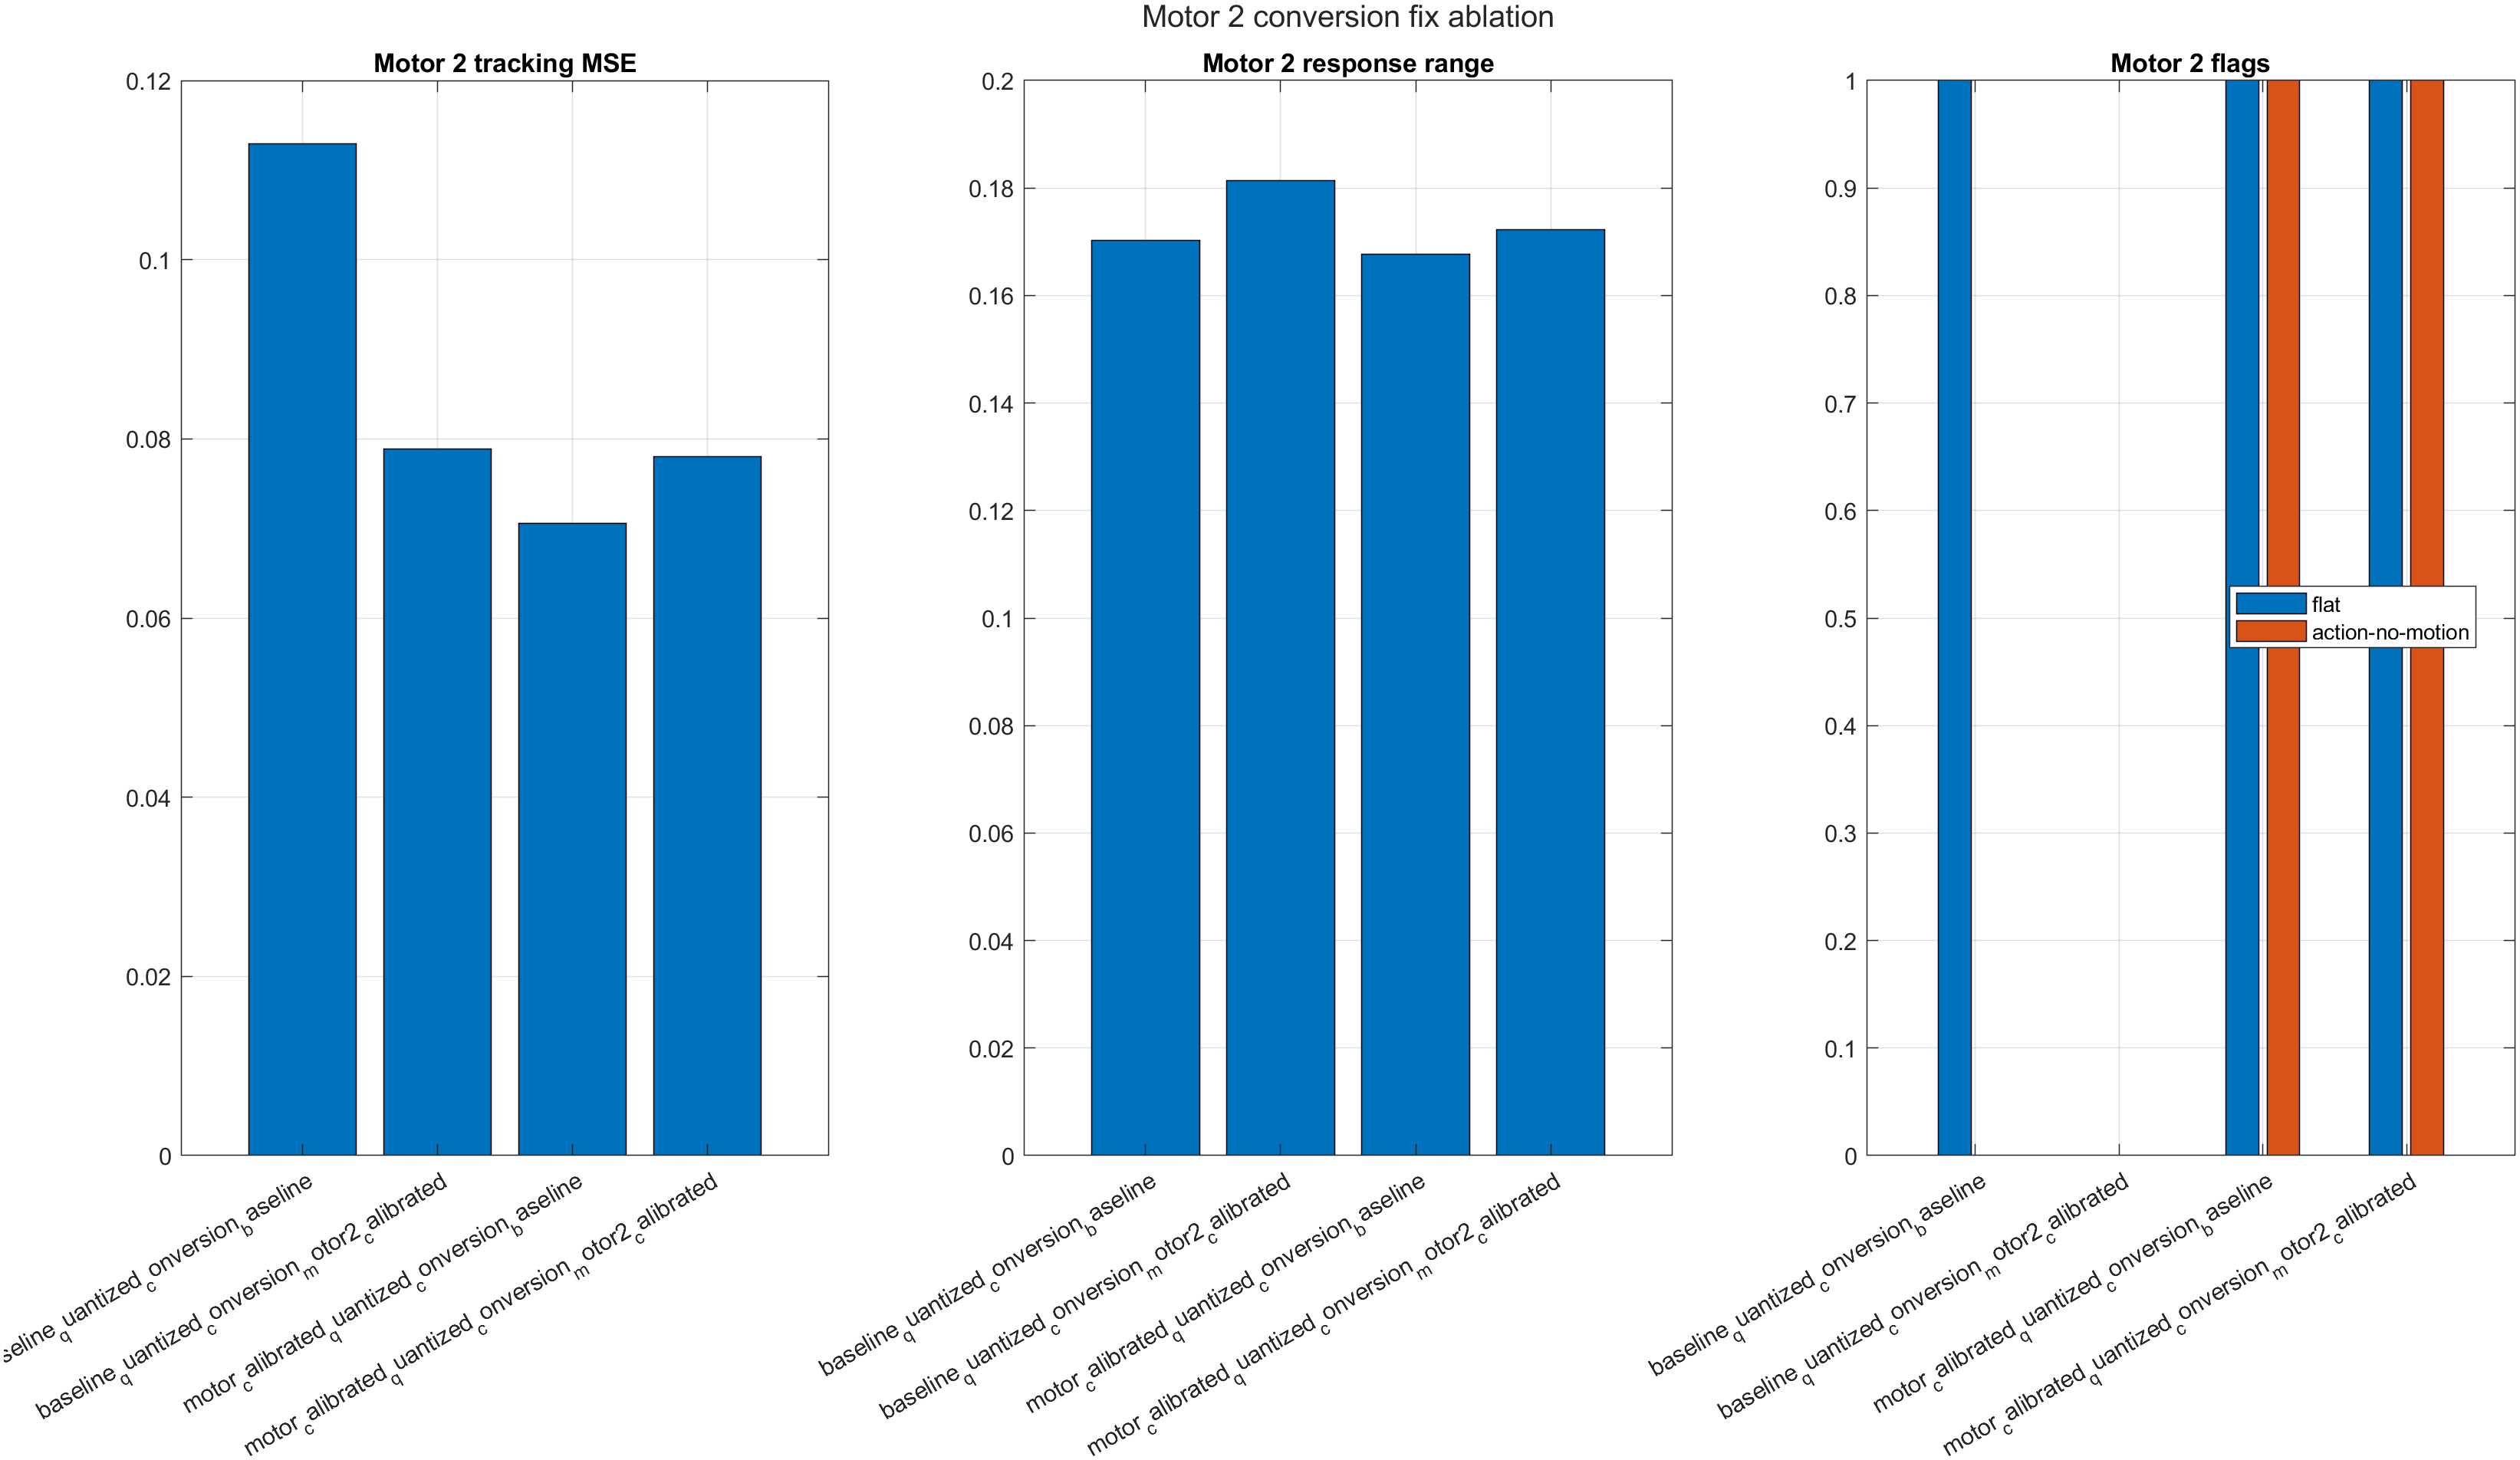
\includegraphics[width=0.92\linewidth]{conversion_fix_ablation_motor2_summary.png}
\caption{Resumen MATLAB de motor 2 con conversion calibrada.}
\end{figure}

\begin{figure}[H]
\centering
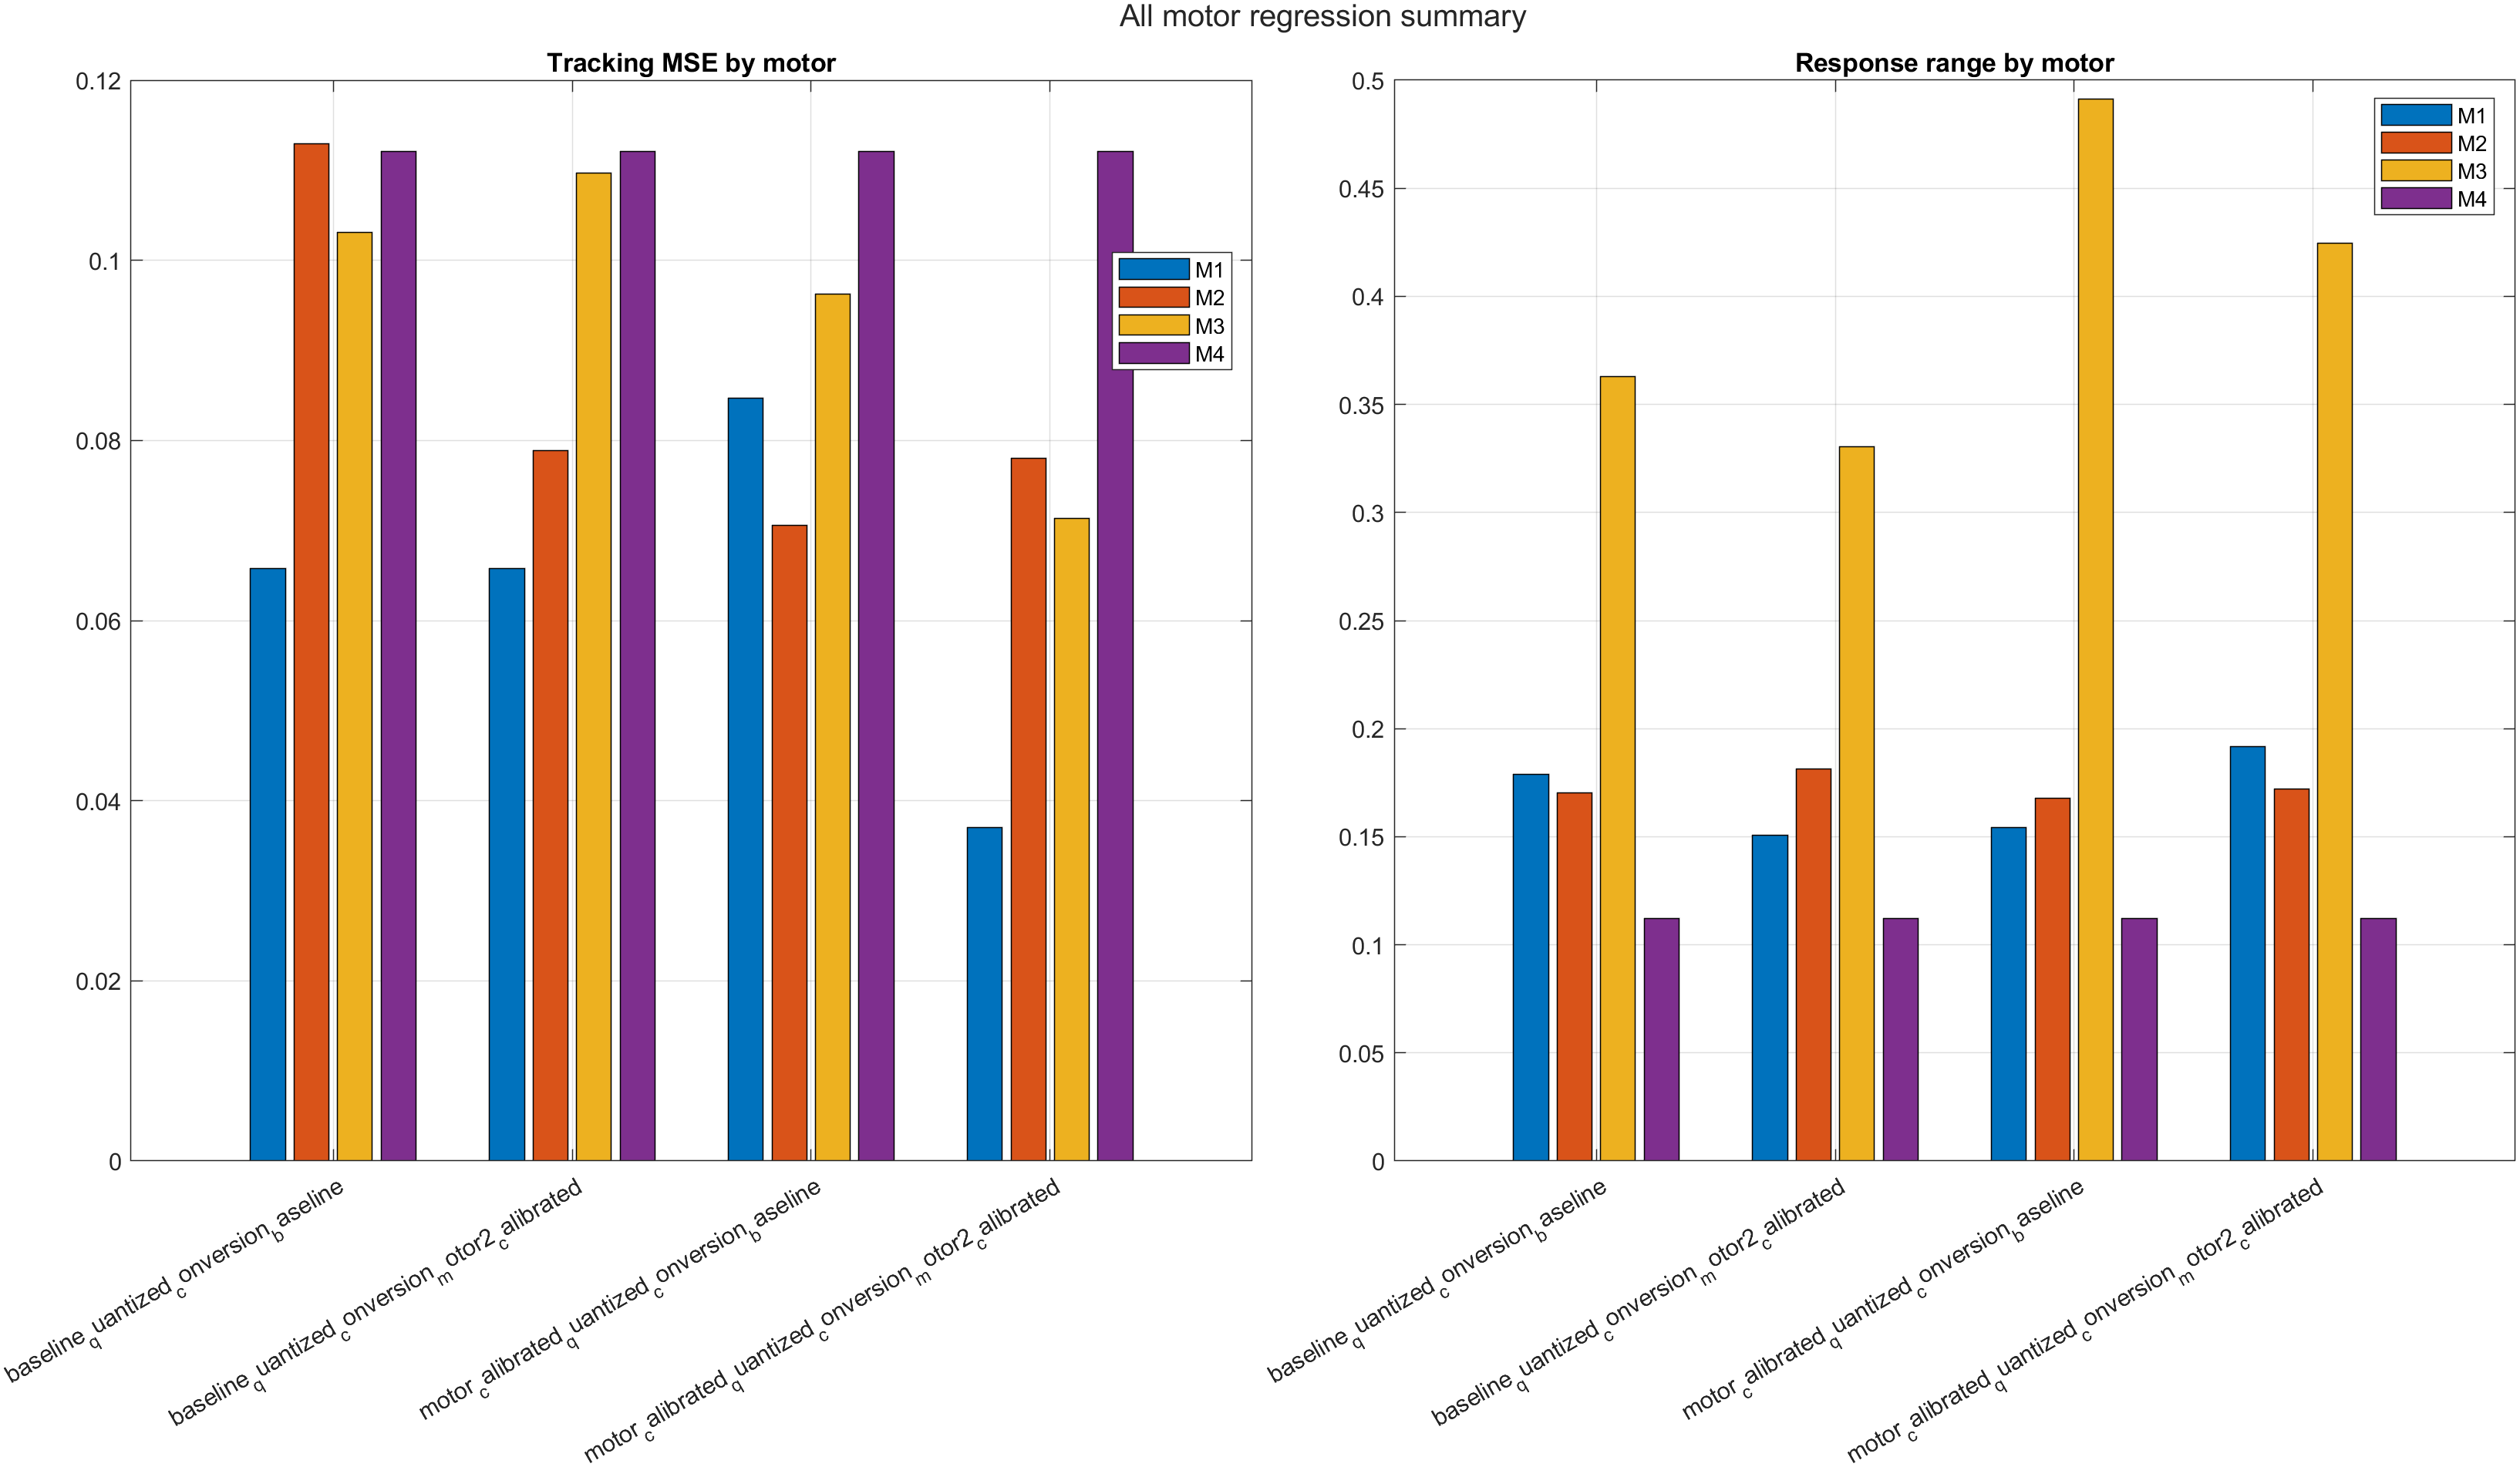
\includegraphics[width=0.92\linewidth]{conversion_fix_ablation_all_motor_summary.png}
\caption{Revision MATLAB de todos los motores en la ablation de conversion.}
\end{figure}

\begin{figure}[H]
\centering
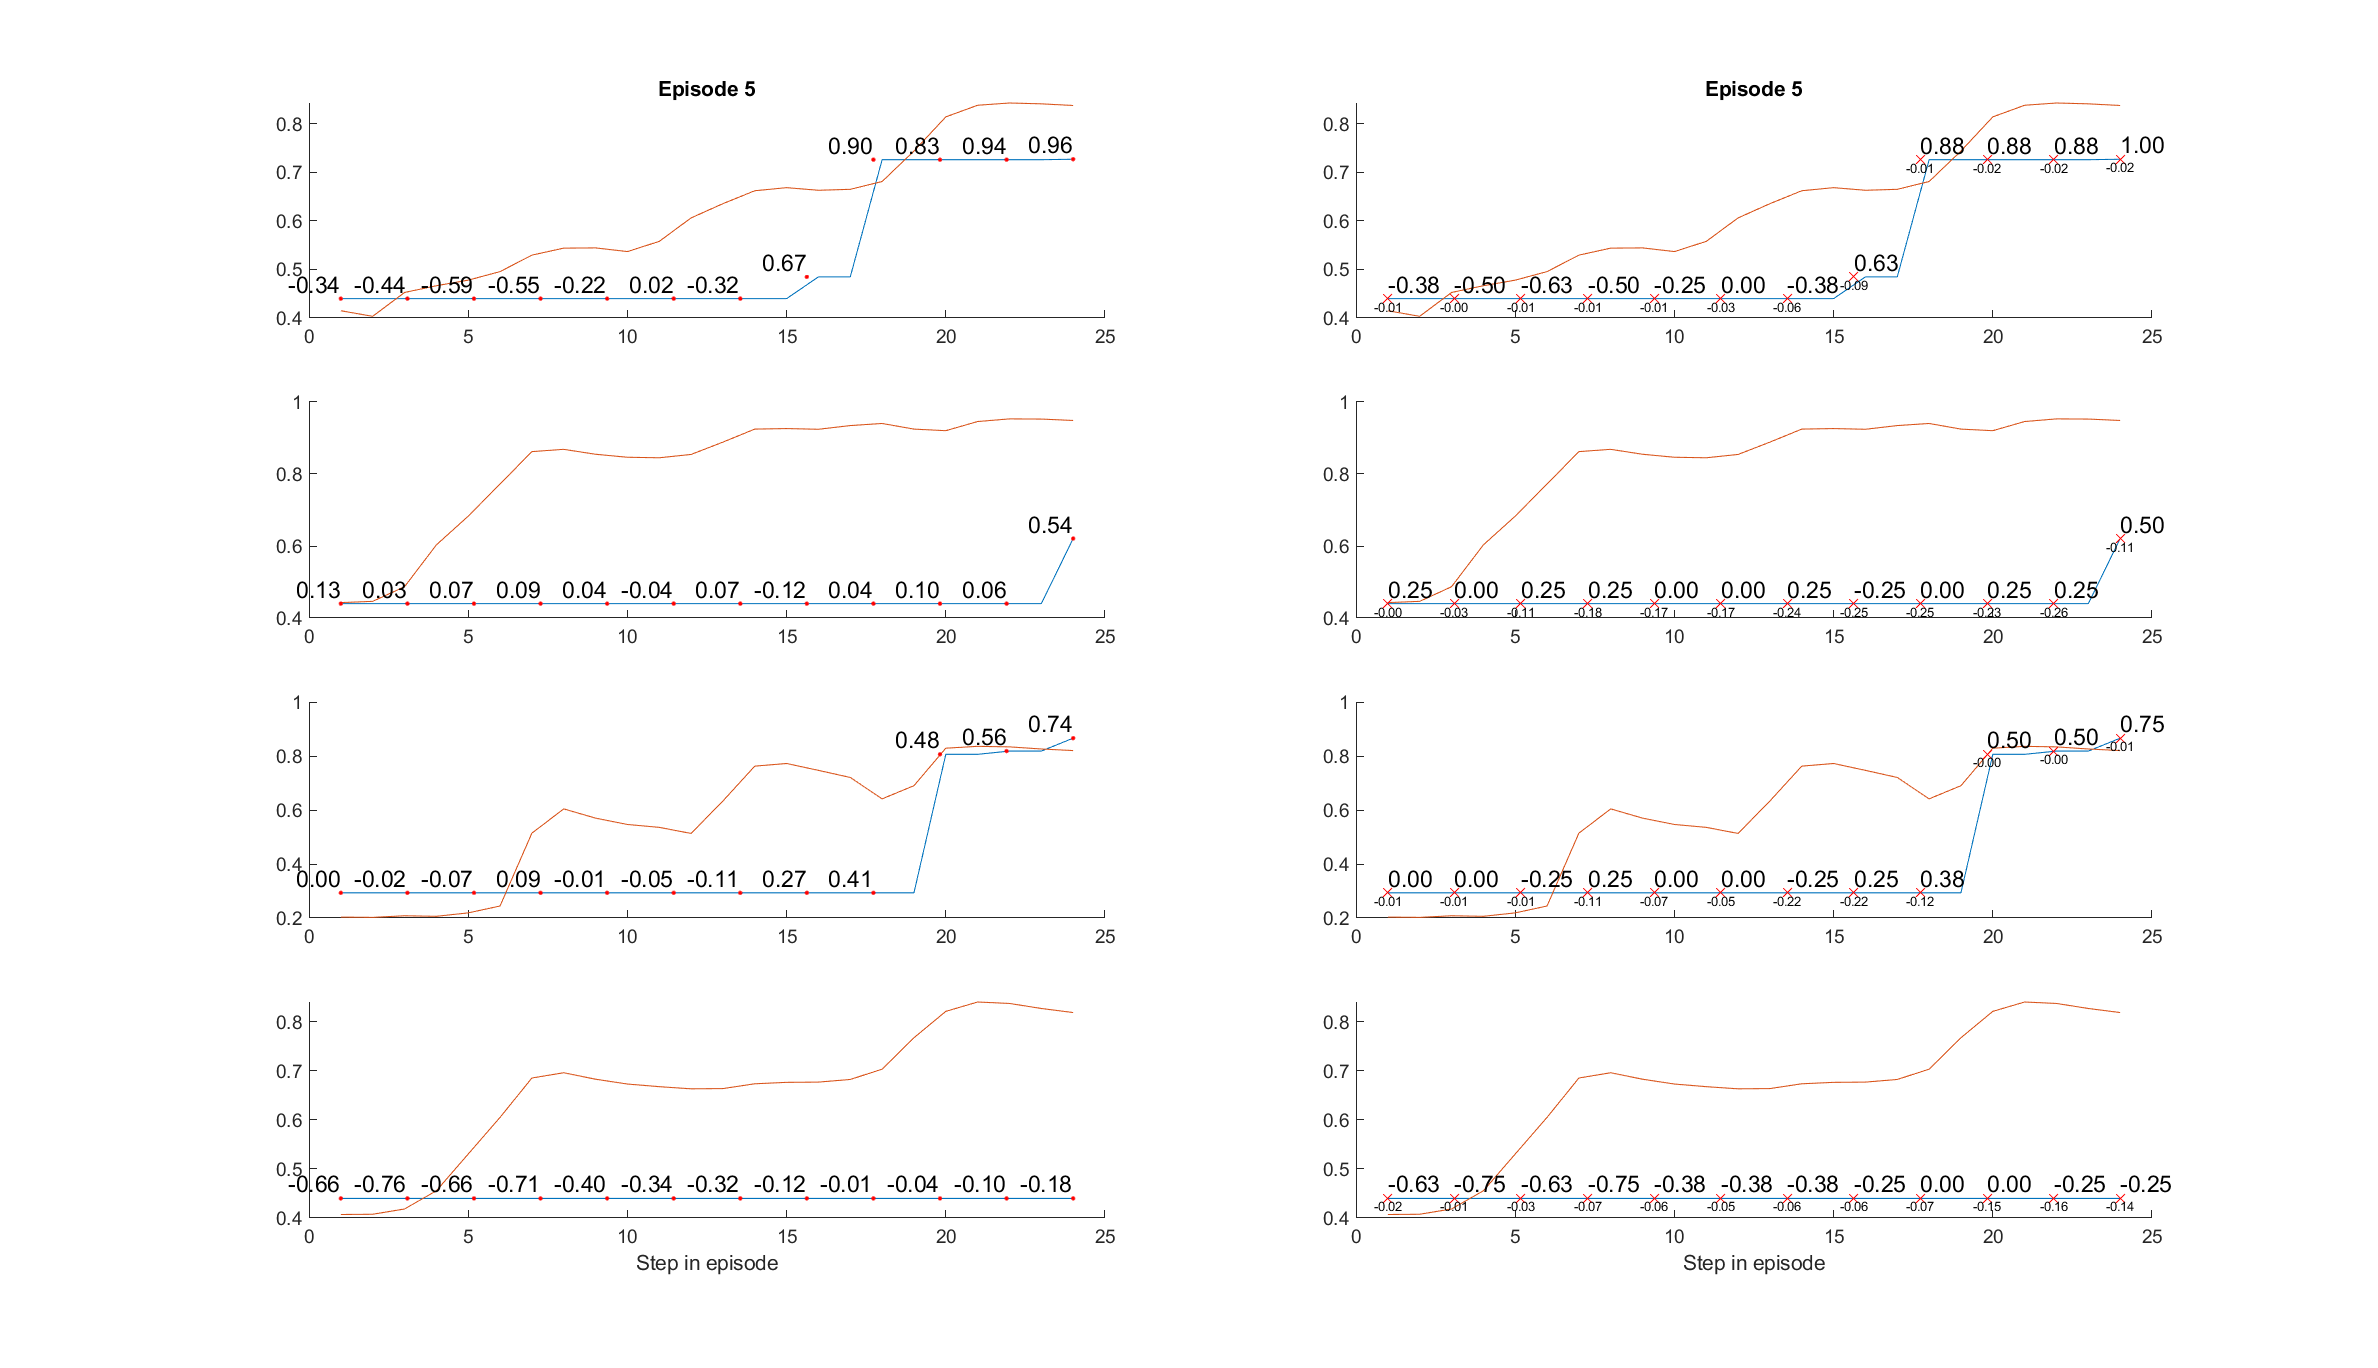
\includegraphics[width=0.92\linewidth]{conversion_fix_seed055_baseline_quantized_motor2_calibrated_visual_test.png}
\caption{Test visual MATLAB, seed 55, conversion experimental, episodio 5.}
\end{figure}

\section{Validacion all-motor}

Luego se reviso una corrida mediana con seeds \texttt{[11 22 55]},
\texttt{1500} episodios de entrenamiento y test final de \texttt{20}
episodios:

\begin{verbatim}
Agentes/motor2_conversion_fix_ablation/26-06-18_09-04-57/
\end{verbatim}

La pregunta cambio. Ya no se evaluo solo si motor 2 mejoraba. Se comparo
\texttt{baseline + baseline} contra \texttt{baseline + motor2Calibrated} en
los cuatro motores, usando tracking, rango de respuesta, saturacion y flags.

\begin{table}[H]
\centering
\caption{Validacion all-motor, baseline contra motor2Calibrated.}
\begin{tabular}{lrrrrrrrr}
\toprule
Motor & MSE B & MSE Cal & Range B & Range Cal & Sat B & Sat Cal & Flat B/Cal & NoMot B/Cal \\
\midrule
M1 & 0.049273 & 0.046642 & 0.158289 & 0.184793 & 0.110094 & 0.410934 & 2/1 & 1/1 \\
M2 & 0.087531 & 0.071070 & 0.155809 & 0.160425 & 0.109722 & 0.105740 & 1/1 & 0/0 \\
M3 & 0.118077 & 0.120305 & 0.428794 & 0.441262 & 0.137444 & 0.090938 & 0/0 & 0/0 \\
M4 & 0.073825 & 0.070127 & 0.149345 & 0.151670 & 0.309727 & 0.415941 & 2/3 & 2/3 \\
\bottomrule
\end{tabular}
\end{table}

Motor 2 mejora en error y rango, pero aun mantiene un flag flat agregado.
Motor 4 no empeora en MSE ni en rango promedio. Sin embargo, si empeora en
saturacion y en conteo de flags: pasa de \texttt{2/3} a \texttt{3/3} tanto
en \texttt{flat} como en \texttt{action-no-motion}. Visualmente, seed 55
mantiene motor 4 casi plano mientras recibe acciones altas/saturadas. Esto
ya aparecia en baseline, pero la variante lo empeora en el conteo de flags.

Por eso la variante no debe aceptarse como ``fix de motor 2'' aislado. La
direccion correcta queda como: \texttt{Motor 2 fix + all-motor regression
validation}. Se agrego \texttt{selectionMode="all\_motor\_final\_gate"} para
que futuras pruebas no acepten un checkpoint si M1, M3 o M4 quedan con
regresion fuerte.

\section{Auditoria all-motor}

La siguiente fase cambia el enfoque a \texttt{All-motor actuation and
regression audit}. El objetivo es separar cuatro posibilidades: selector de
checkpoint que prioriza motor 2, problema de conversion o mapeo en motor 4,
saturacion con poca respuesta, y figuras antiguas mal asociadas a
configuraciones.

Se agrego la bandera \texttt{high\_action\_flat\_response\_motorK}. Esta
bandera se activa cuando un motor recibe accion alta o saturacion alta,
pero su rango de respuesta queda bajo mientras la referencia si cambia. Esta
bandera captura el caso visual observado en motor 4.

El selector \texttt{all\_motor\_final\_gate} queda como gate estricto. Si
ningun checkpoint pasa los cuatro motores, el flujo selecciona el menos malo
solo para diagnostico, deja \texttt{finalGateAccepted=false} y usa la razon
\texttt{fallback\_diagnostic\_no\_checkpoint\_passed\_all\_motor\_gate}.

Tambien se agregaron tres launchers sin campana larga:

\begin{verbatim}
run_all_motor_visual_comparison_from_run
run_all_motor_actuation_sanity_check_extended
run_compare_against_canonical_benchmark_all_motor
\end{verbatim}

Las nuevas figuras visuales deben incluir seed, episodio,
\texttt{actionInterfaceVariant}, \texttt{encoder2FlexVariant},
\texttt{selectionMode}, checkpoint y carpeta de corrida. No se deben usar
figuras antiguas sin metadata clara para aceptar la variante.

La auditoria generada el 2026-06-19 dejo una lectura mas clara. En el
sanity controlado, motor 4 muestra zona muerta y asimetria, pero sus
resultados son iguales con conversion baseline y con
\texttt{motor2Calibrated}. Esto indica que la conversion local de motor 2 no
modifica directamente el actuador M4. En cambio, los checkpoints entrenados
si muestran M4 plano en varias seeds, especialmente cuando hay saturacion
alta.

En la comparacion contra \texttt{Agent7250}, el benchmark historico no
disparo flags en motor 4 durante el test de 20 episodios:
\texttt{trackingMSE\_motor4=0.030795},
\texttt{responseRange\_motor4=0.198918} y
\texttt{saturationFraction\_motor4=0.278977}. Por tanto, el problema visual
de M4 parece estar mas asociado al entrenamiento, selector o reward de los
checkpoints nuevos que a la conversion \texttt{motor2Calibrated} por si
sola.

\begin{figure}[H]
\centering
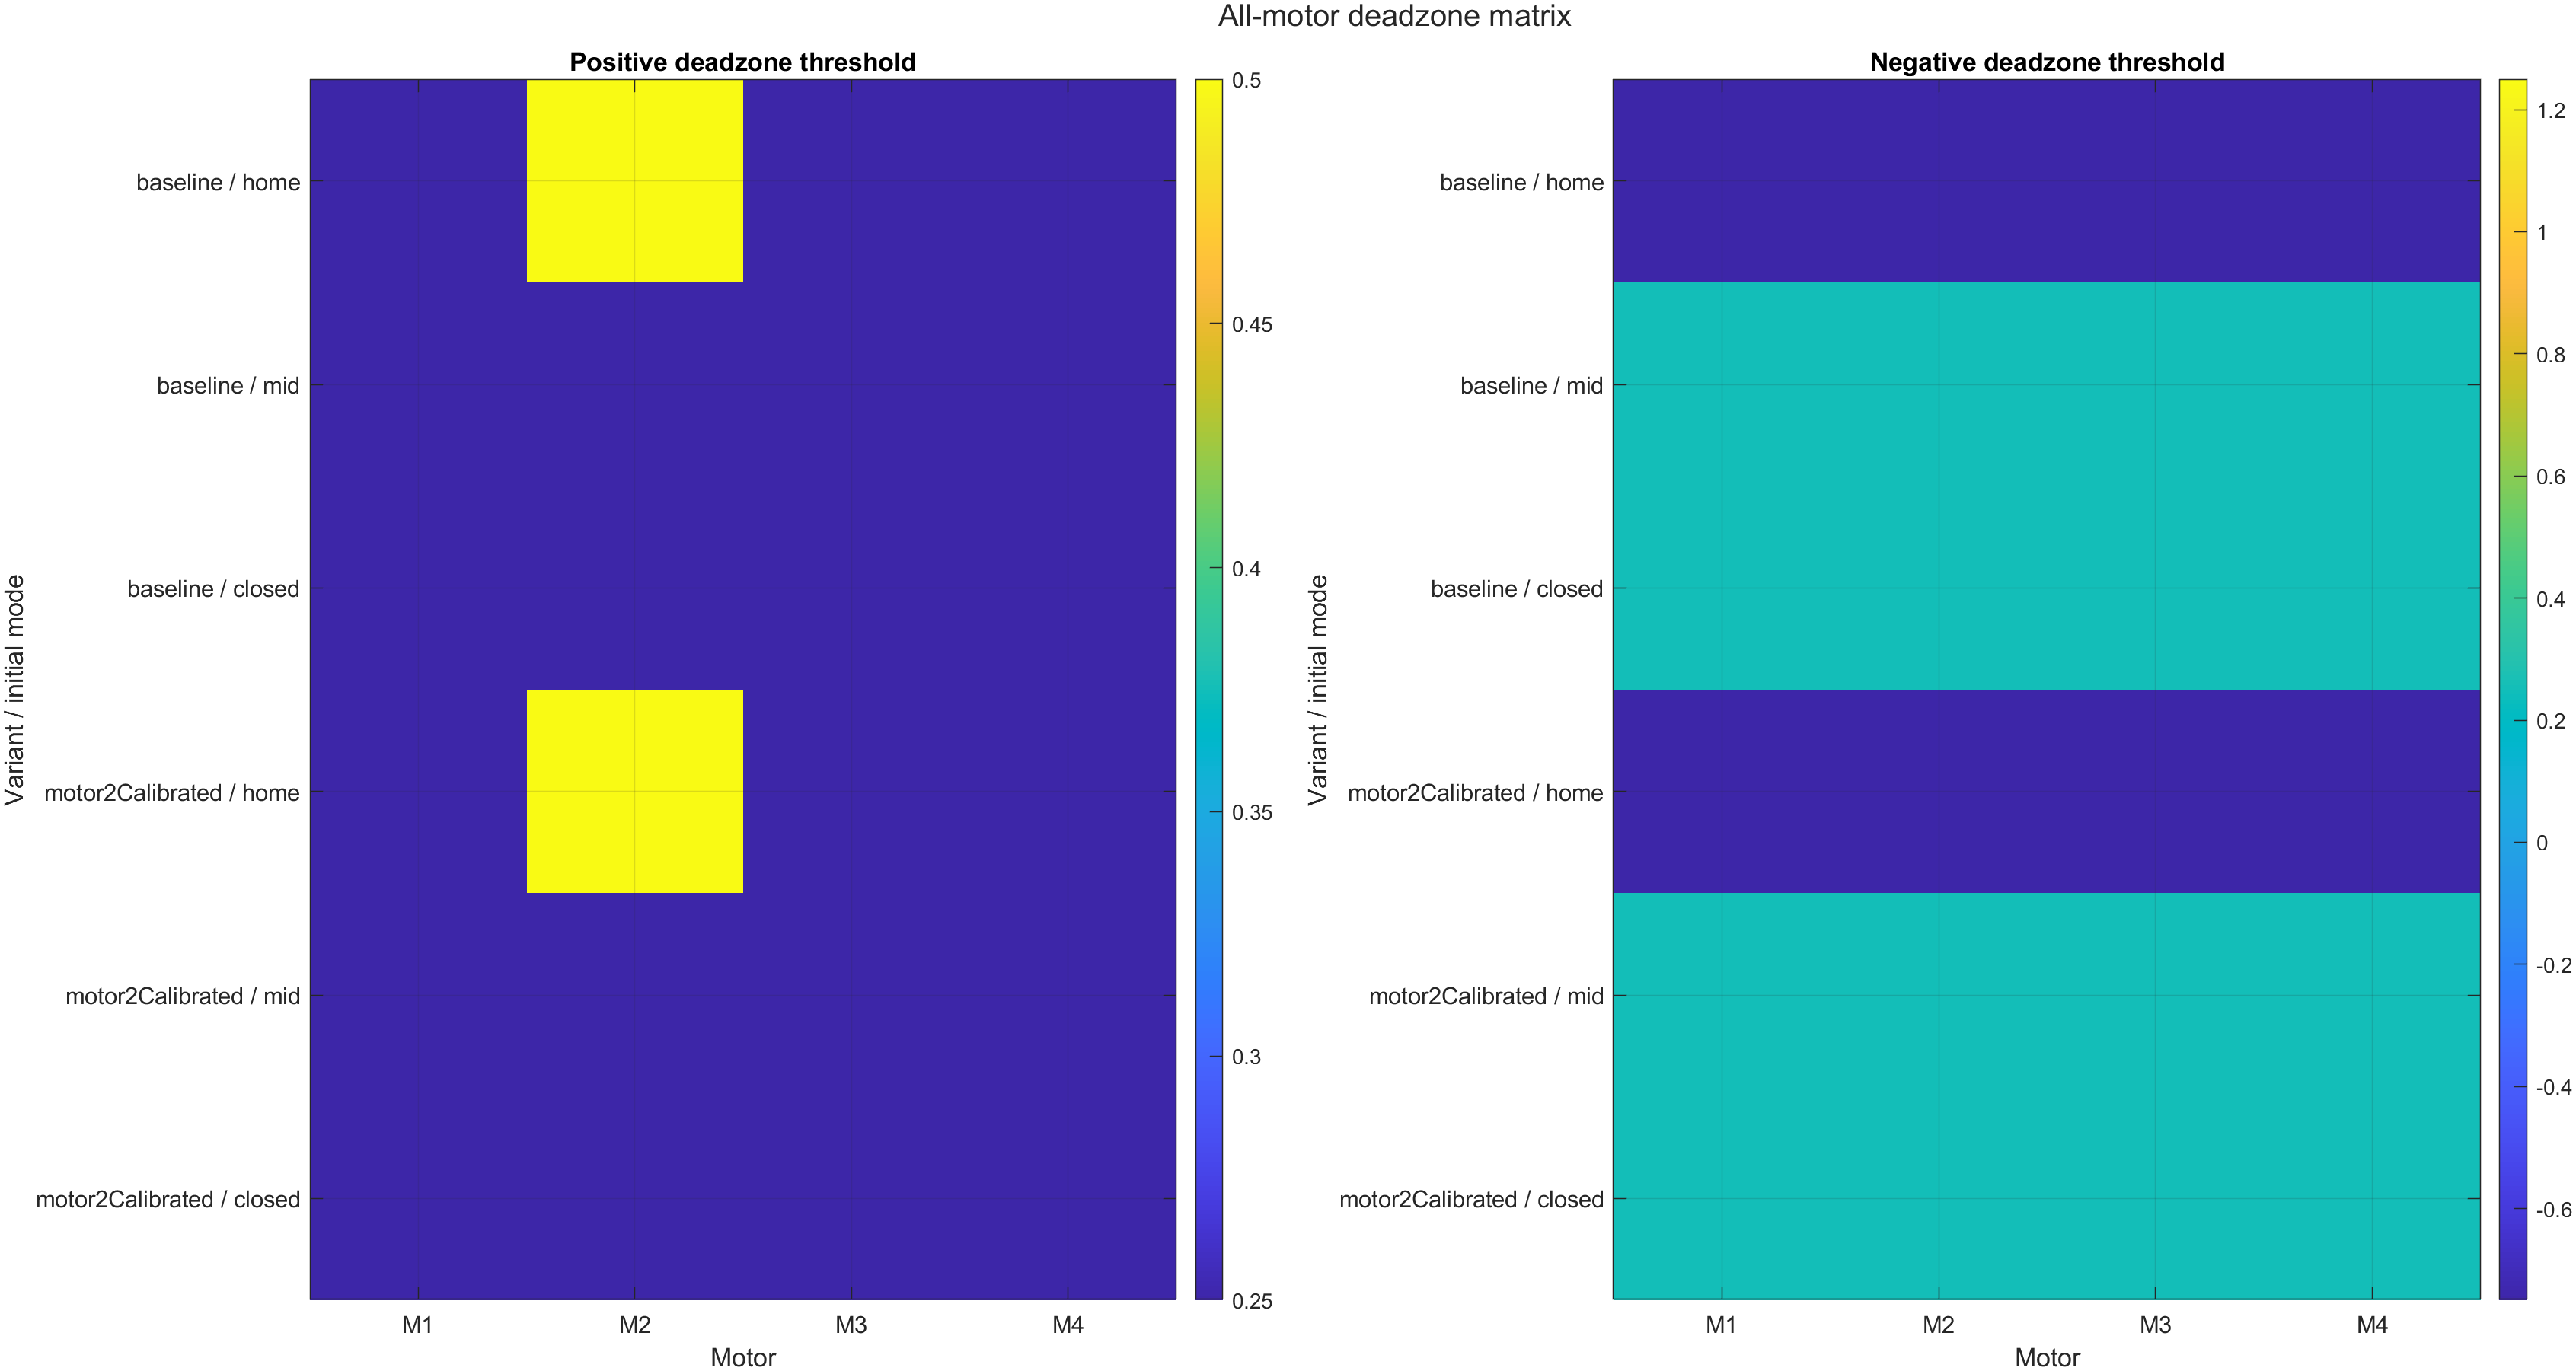
\includegraphics[width=0.92\linewidth]{all_motor_review/all_motor_deadzone_matrix.png}
\caption{Sanity MATLAB all-motor: deadzone por motor, posicion inicial y variante de conversion.}
\end{figure}

\begin{figure}[H]
\centering
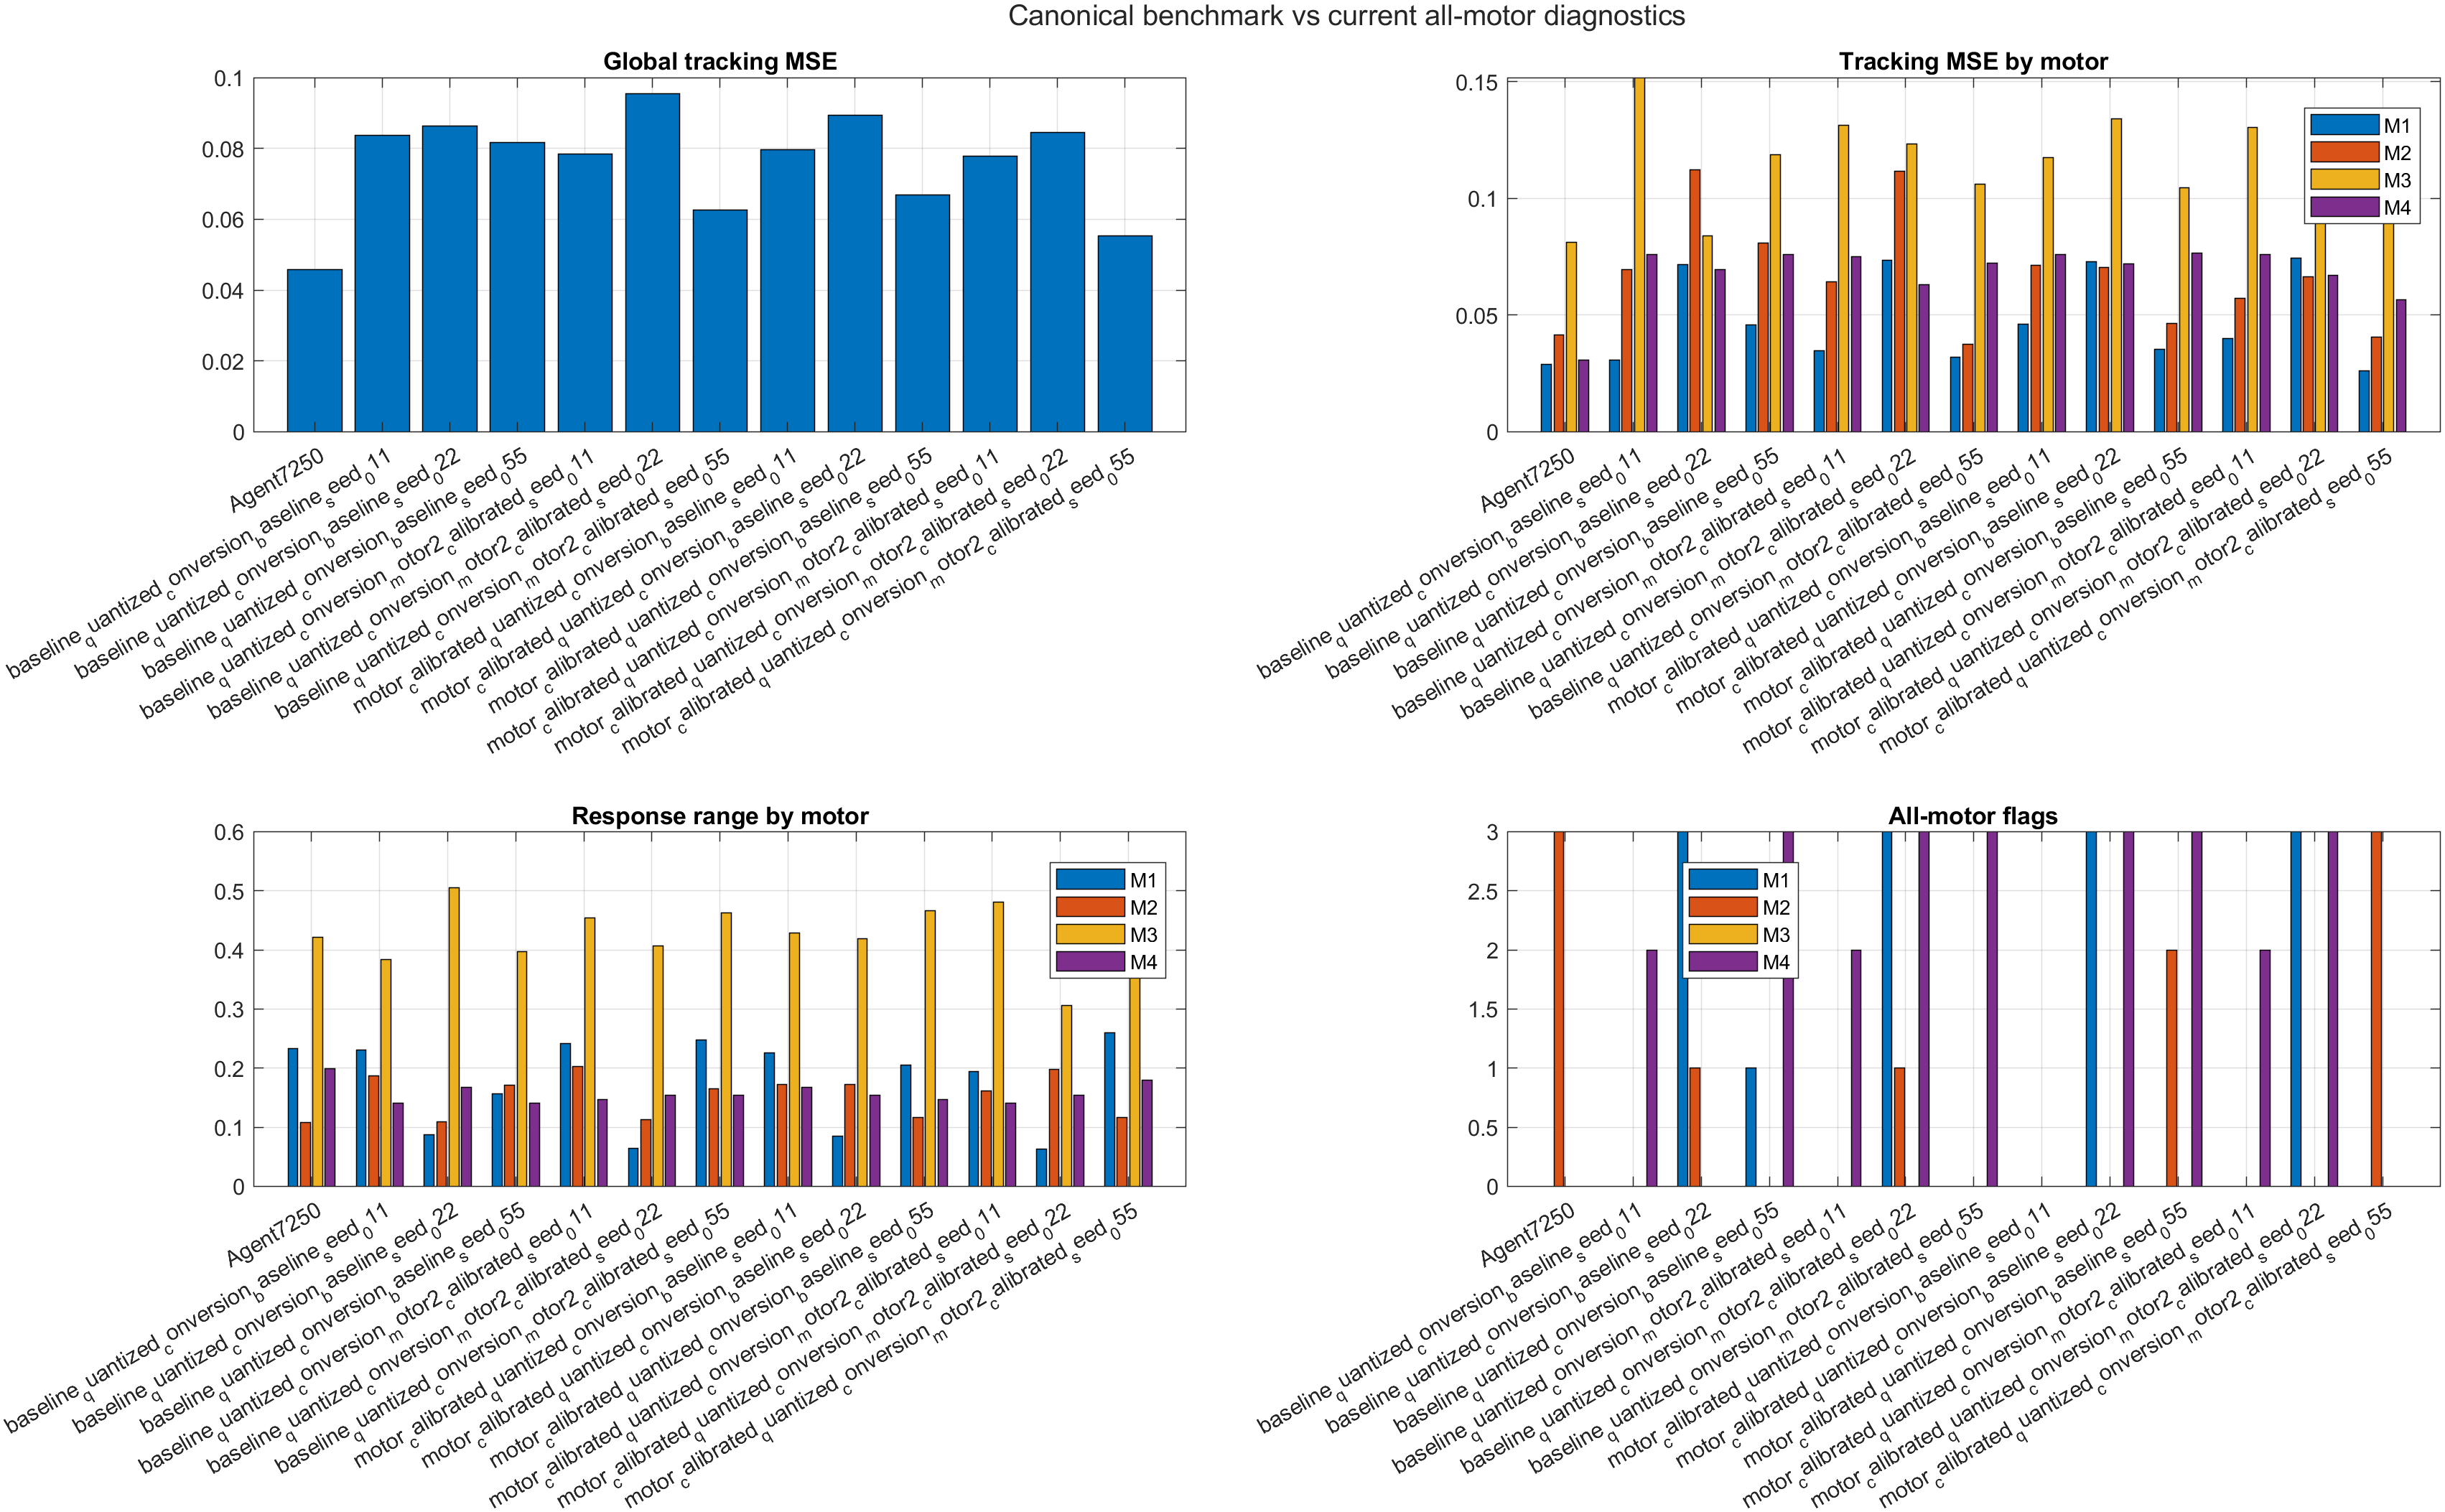
\includegraphics[width=0.92\linewidth]{all_motor_review/canonical_vs_current_all_motor.png}
\caption{Comparacion MATLAB de \texttt{Agent7250} contra checkpoints actuales con metricas M1-M4.}
\end{figure}

\section{Validacion corta all-motor del 2026-06-22}

Se ejecuto una validacion corta con seeds \texttt{[11 55]},
\texttt{300} episodios de entrenamiento, test final de \texttt{5}
episodios, \texttt{auditTopK=4}, \texttt{gapOffset=-256} y
\texttt{selectionMode="all\_motor\_final\_gate"}.

\begin{verbatim}
Agentes/motor2_conversion_fix_ablation/26-06-22_09-21-51/
\end{verbatim}

\begin{table}[H]
\centering
\caption{Validacion corta all-motor, baseline contra motor2Calibrated.}
\begin{tabular}{lrrrrrrrrr}
\toprule
Motor & MSE B & MSE Cal & Range B & Range Cal & Sat B & Sat Cal & Flat & NoMot & HiActFlat \\
\midrule
M1 & 0.066164 & 0.080685 & 0.142948 & 0.152240 & 0.004167 & 0.004167 & 1/1 & 1/1 & 0/0 \\
M2 & 0.141460 & 0.100132 & 0.130941 & 0.169585 & 0.020833 & 0.016667 & 2/0 & 0/0 & 0/0 \\
M3 & 0.101131 & 0.102842 & 0.370884 & 0.387618 & 0.000000 & 0.000000 & 0/0 & 0/0 & 0/0 \\
M4 & 0.112090 & 0.112090 & 0.112263 & 0.112263 & 0.369231 & 0.000000 & 2/2 & 2/2 & 1/0 \\
\bottomrule
\end{tabular}
\end{table}

La configuracion \texttt{baselineQuantized + motor2Calibrated} mejoro motor
2: bajo \texttt{trackingMSE\_motor2}, subio
\texttt{responseRange\_motor2} y elimino los flags de motor 2. Tambien bajo
la saturacion global de \texttt{0.100641} a \texttt{0.006250} y elimino la
bandera \texttt{high\_action\_flat} de motor 4.

La mejora no fue suficiente para aceptar la variante. Motor 1 empeoro en
MSE y motor 4 siguio con \texttt{flat 2/2} y
\texttt{action-no-motion 2/2}. Todas las configuraciones quedaron con
\texttt{acceptedConversion=0}. El selector estricto uso fallback diagnostico
porque ningun checkpoint paso M1-M4.

\begin{figure}[H]
\centering
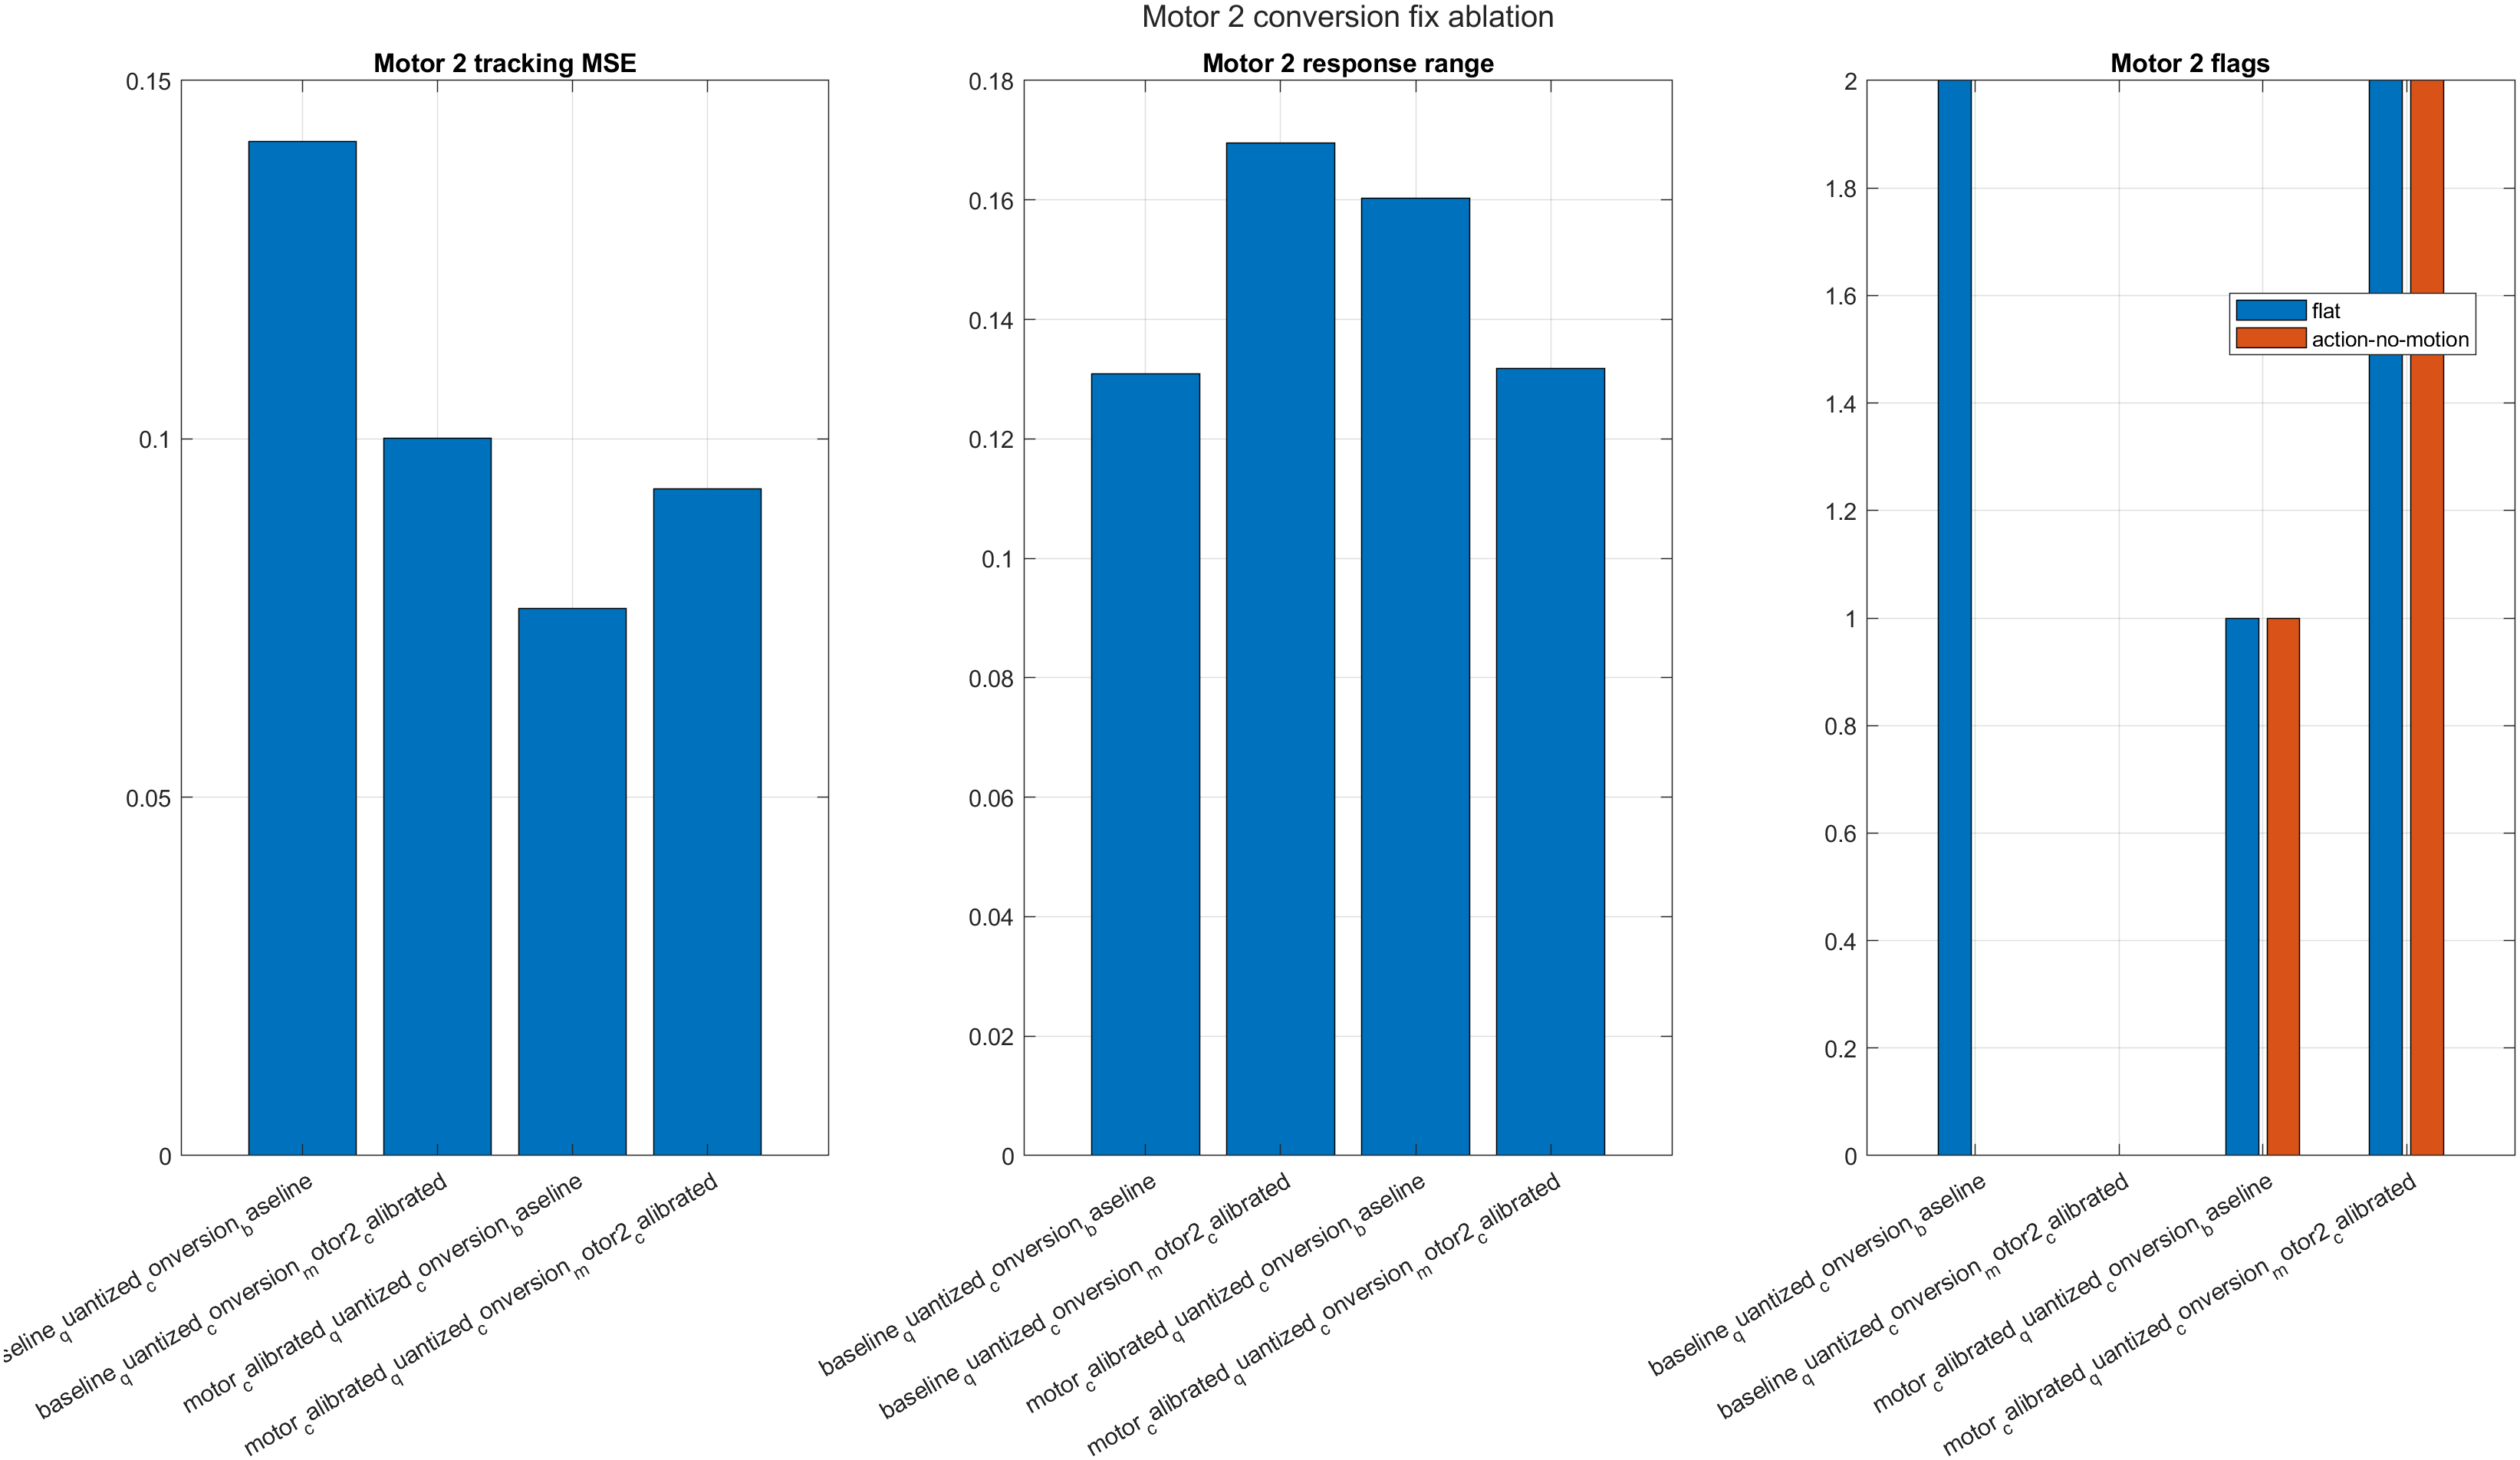
\includegraphics[width=0.92\linewidth]{all_motor_review/conversion_fix_20260622_motor2_summary.png}
\caption{Resumen MATLAB de motor 2 en la validacion corta del 2026-06-22.}
\end{figure}

\begin{figure}[H]
\centering
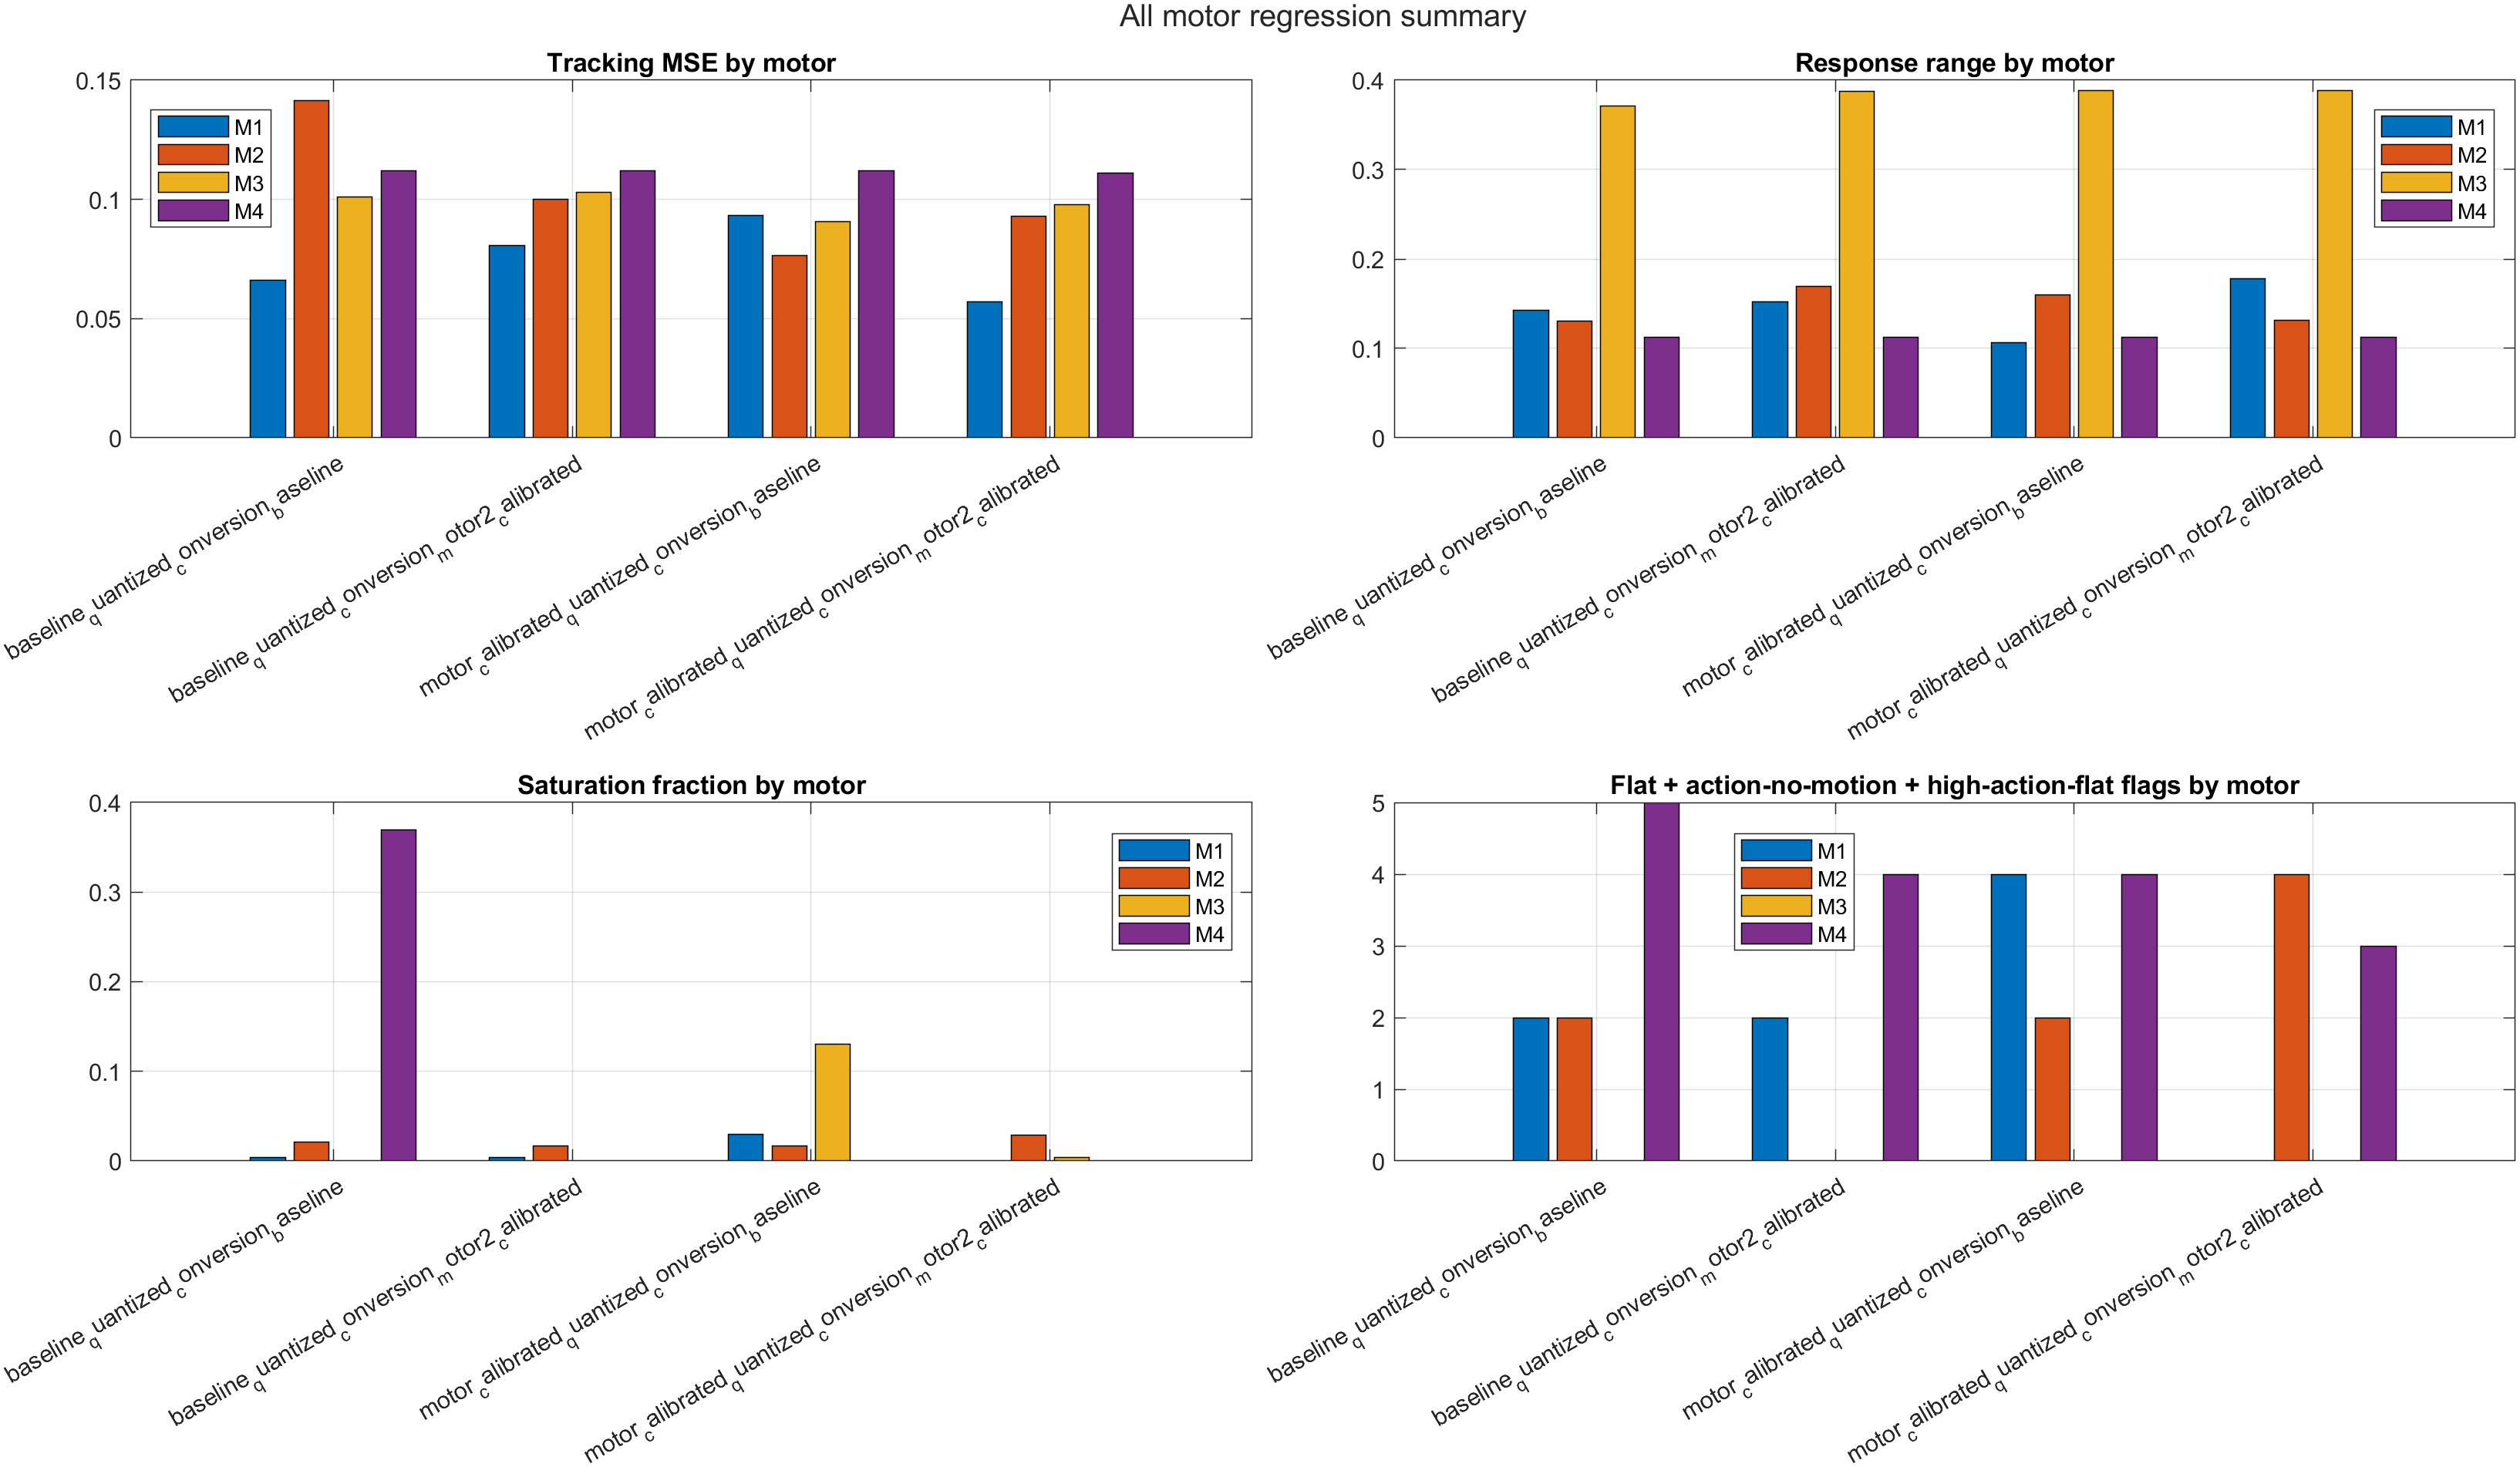
\includegraphics[width=0.92\linewidth]{all_motor_review/conversion_fix_20260622_all_motor_summary.png}
\caption{Resumen MATLAB all-motor en la validacion corta del 2026-06-22.}
\end{figure}

\section{Agent7250 congelado y correccion aislada de motor 2}

Se verifico que las ablations anteriores entrenaban TD3 desde cero. En esas
corridas, \texttt{Agent7250} se usaba como referencia historica, no como
politica base congelada. Por eso se separo la conversion del entrenamiento.

La validacion final se ejecuto sin aprendizaje, con 50 episodios, sin tocar
puertos COM y usando solo simulacion con dataset pregrabado.

\begin{table}[H]
\centering
\caption{Agent7250 congelado con variantes de conversion, 50 episodios.}
\scriptsize
\begin{tabular}{lrrrrrrrr}
\toprule
Config & MSE & MSE M2 & Range M2 & Flags M2 & MSE M4 & Range M4 & Flags M4 & Aceptada \\
\midrule
Baseline & 0.037229 & 0.042474 & 0.109618 & 3 & 0.026250 & 0.231700 & 0 & no \\
M2Cal 0 & 0.037229 & 0.042474 & 0.109618 & 3 & 0.026250 & 0.231700 & 0 & no \\
M2Cal -64 & 0.037113 & 0.041993 & 0.110996 & 3 & 0.026250 & 0.231700 & 0 & no \\
M2Cal -128 & 0.037003 & 0.041534 & 0.112352 & 3 & 0.026250 & 0.231700 & 0 & no \\
M2Cal -256 & 0.036800 & 0.040681 & 0.115000 & 3 & 0.026250 & 0.231700 & 0 & no \\
\bottomrule
\end{tabular}
\end{table}

La conversion \texttt{motor2Calibrated} no degrado M4 cuando
\texttt{Agent7250} quedo congelado. Esto indica que la regresion previa de
M4 viene mas del entrenamiento desde cero, del selector o de la reward. Aun
asi, no se acepta la conversion: motor 2 mejora en MSE y rango, pero conserva
3 flags.

\begin{figure}[H]
\centering
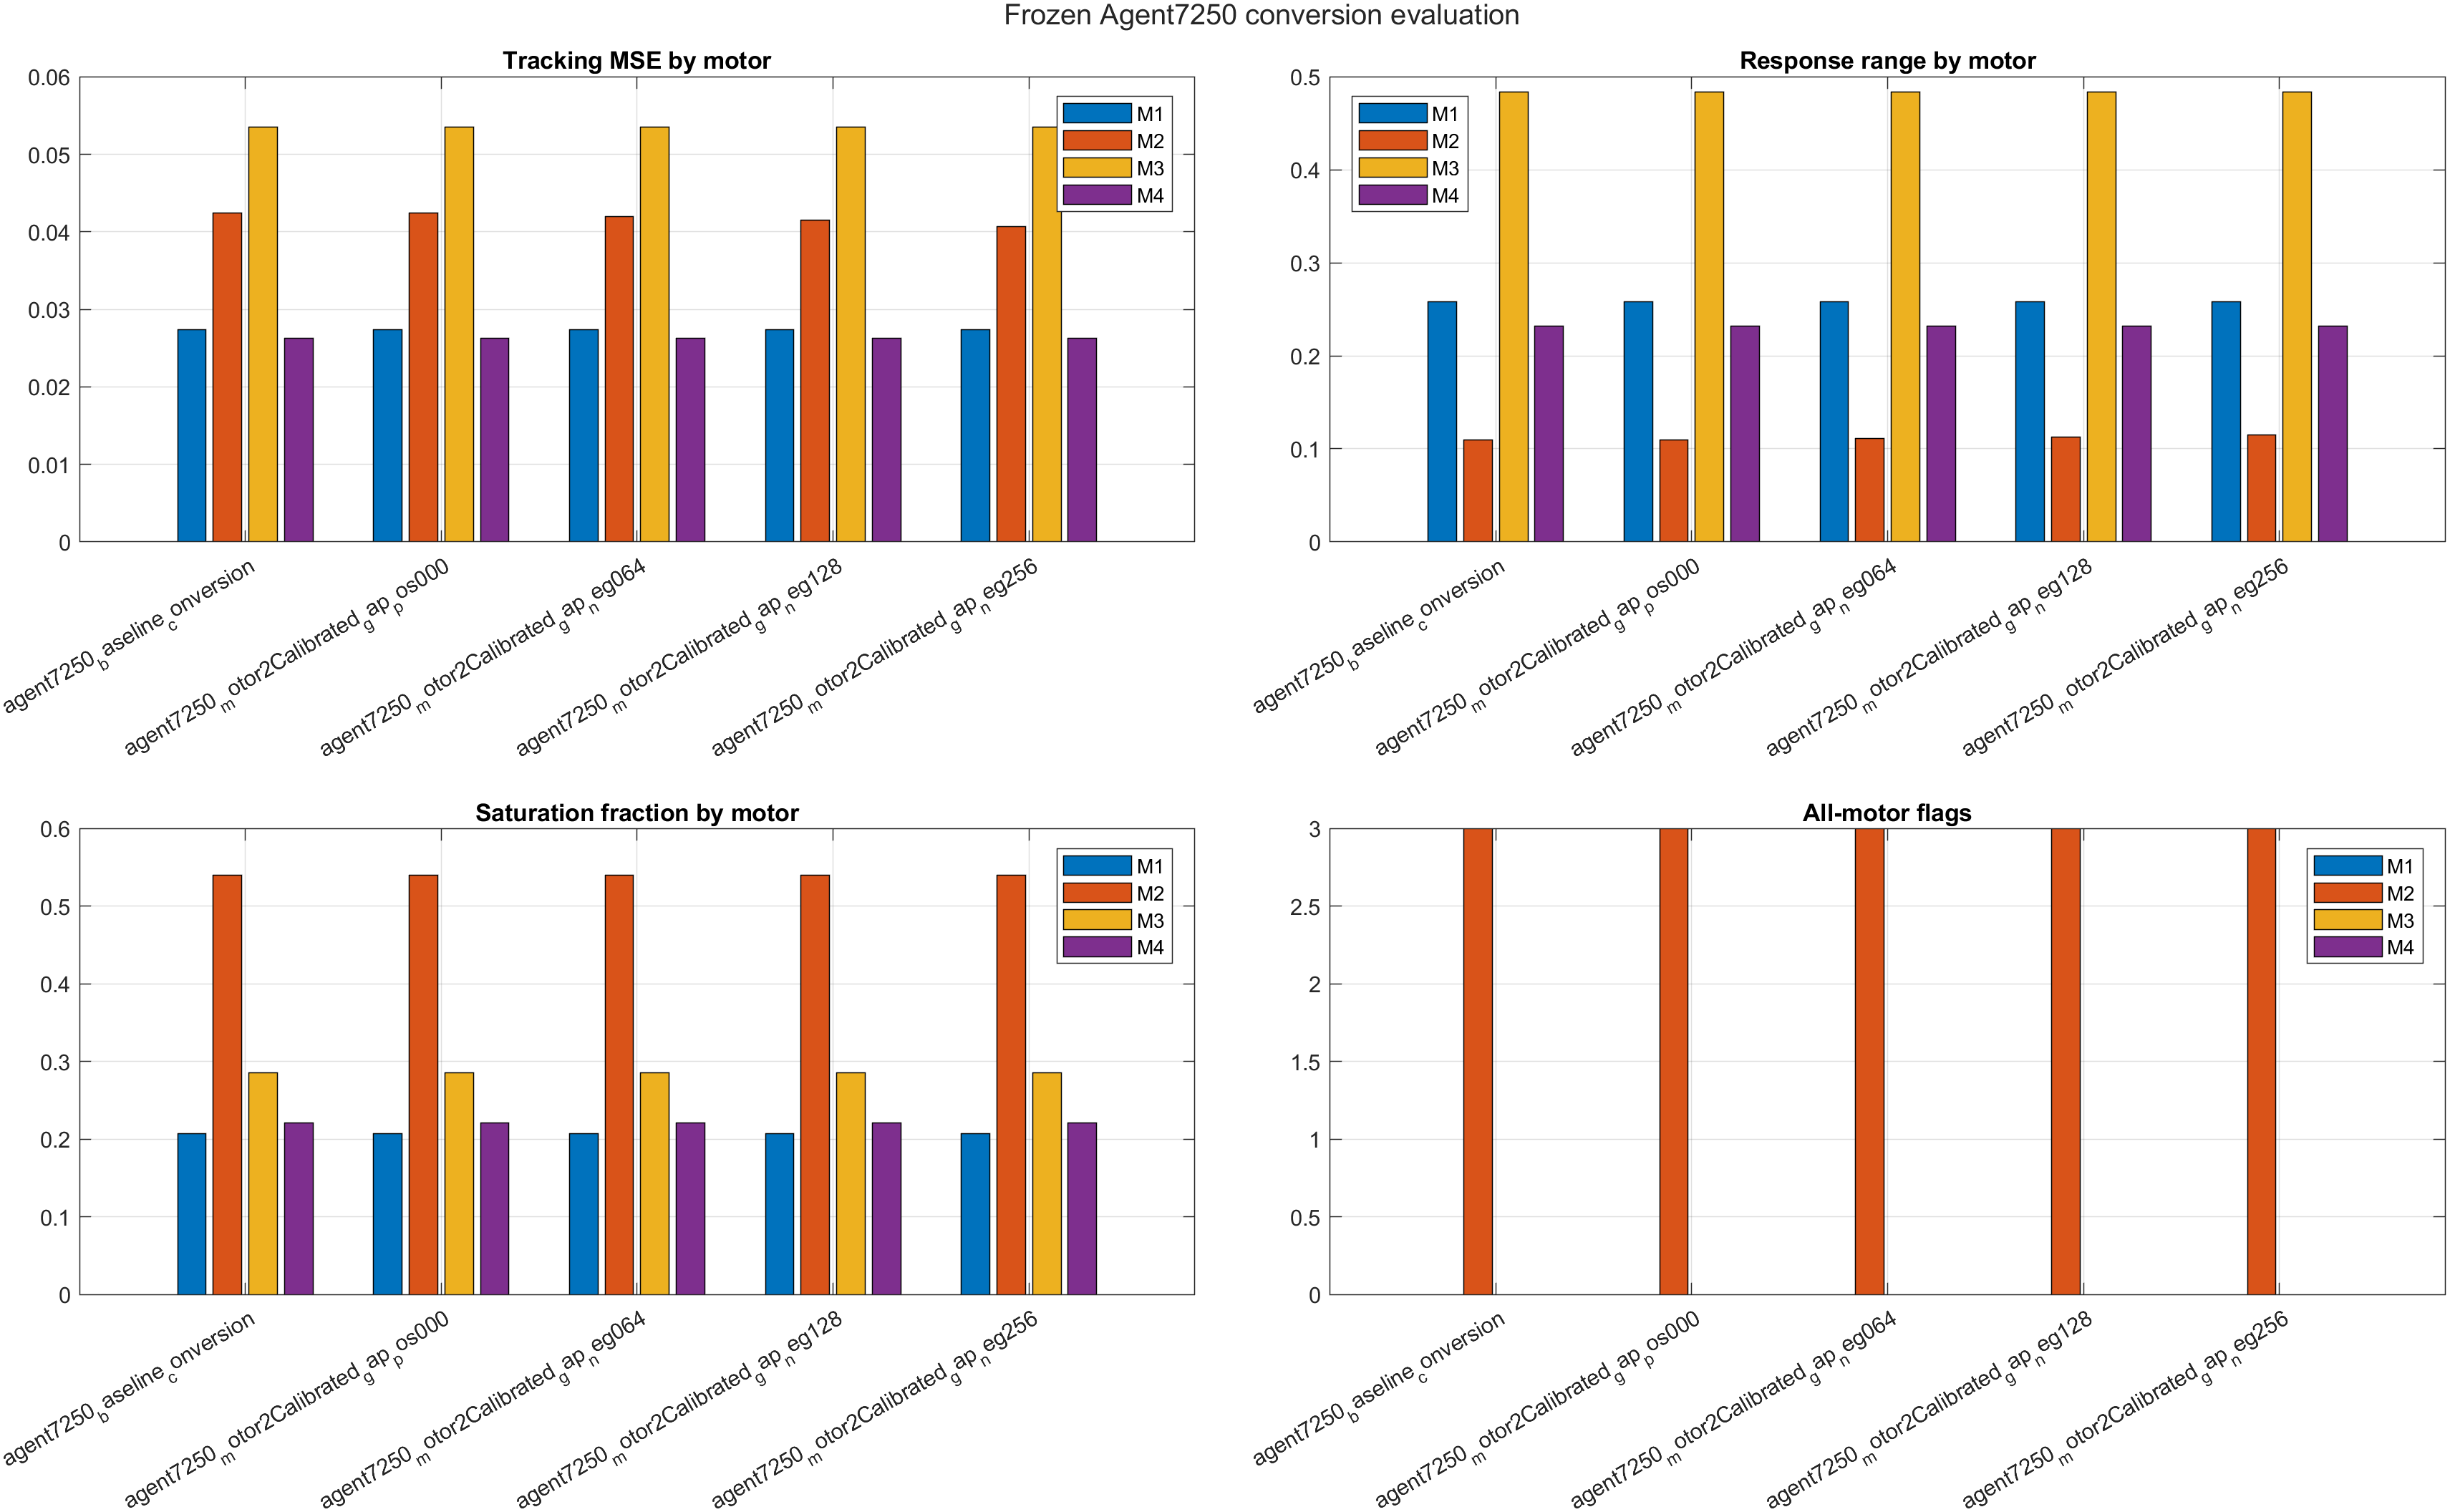
\includegraphics[width=0.92\linewidth]{frozen_agent7250_final/agent7250_frozen_all_motor_comparison_20260623_episode50.png}
\caption{Comparacion MATLAB all-motor con \texttt{Agent7250} congelado, 50 episodios.}
\end{figure}

Luego se probo una correccion heuristica aislada. Esta correccion solo puede
cambiar \texttt{action(2)}. Las acciones de M1, M3 y M4 deben quedar iguales a
la politica base. En la corrida, \texttt{maxNonMotor2ActionDelta=0}.

\begin{table}[H]
\centering
\caption{Agent7250 congelado con correccion aislada de motor 2, 50 episodios.}
\scriptsize
\begin{tabular}{lrrrrrrrrr}
\toprule
Config & MSE & MSE M2 & Range M2 & Flags M2 & MSE M4 & Range M4 & Flags M4 & non-M2 & Aceptada \\
\midrule
Baseline & 0.037229 & 0.042474 & 0.109618 & 3 & 0.026250 & 0.231700 & 0 & 0 & no \\
M2Cal -256 & 0.036800 & 0.040681 & 0.115000 & 3 & 0.026250 & 0.231700 & 0 & 0 & no \\
M2 heuristic & 0.037127 & 0.042015 & 0.110570 & 3 & 0.025986 & 0.231700 & 0 & 0 & no \\
M2 heuristic + M2Cal & 0.036692 & 0.040224 & 0.115923 & 3 & 0.025986 & 0.231700 & 0 & 0 & no \\
\bottomrule
\end{tabular}
\end{table}

La correccion aislada preservo M1, M3 y M4. Tambien bajo el MSE global,
bajo el MSE de motor 2 y subio el rango de motor 2. Pero no se acepta porque
los flags de motor 2 siguen presentes. La regla final no permite aceptar una
variante que mejora metricas pero conserva flags.

\begin{figure}[H]
\centering
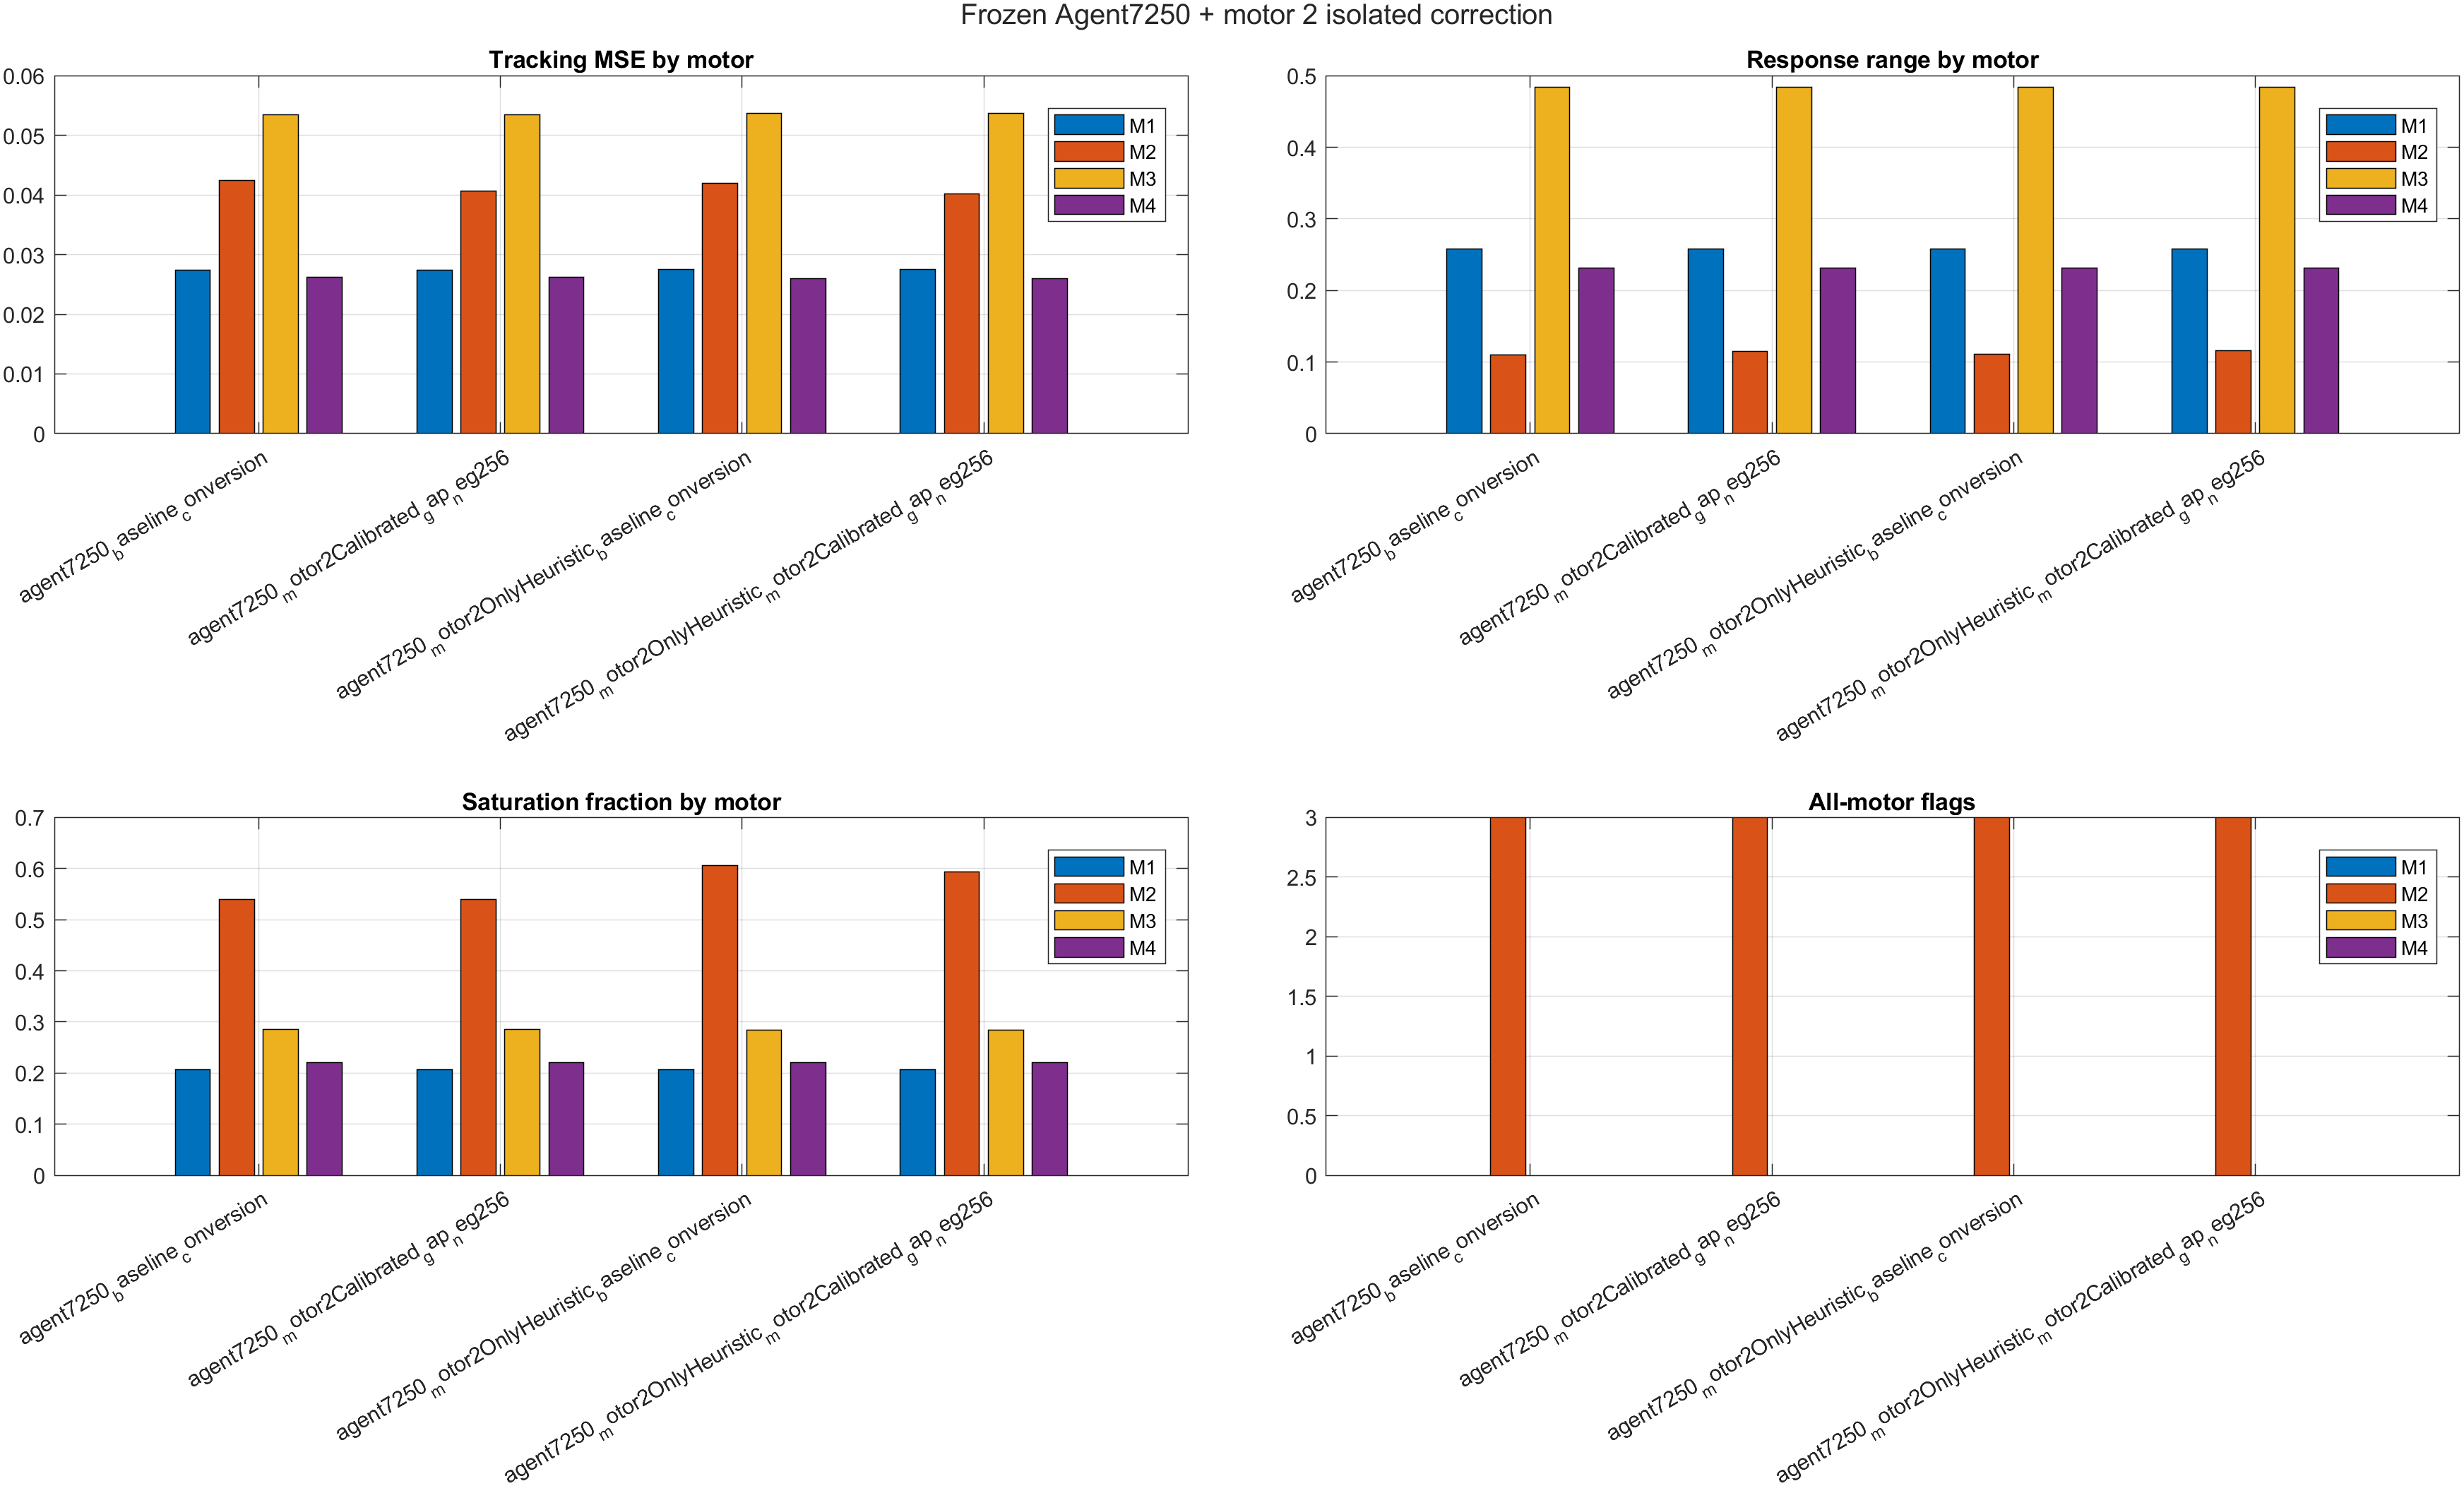
\includegraphics[width=0.92\linewidth]{frozen_agent7250_final/agent7250_motor2_only_correction_all_motor_comparison_20260623_episode50.png}
\caption{Comparacion MATLAB all-motor con correccion aislada de motor 2, 50 episodios.}
\end{figure}

\begin{figure}[H]
\centering
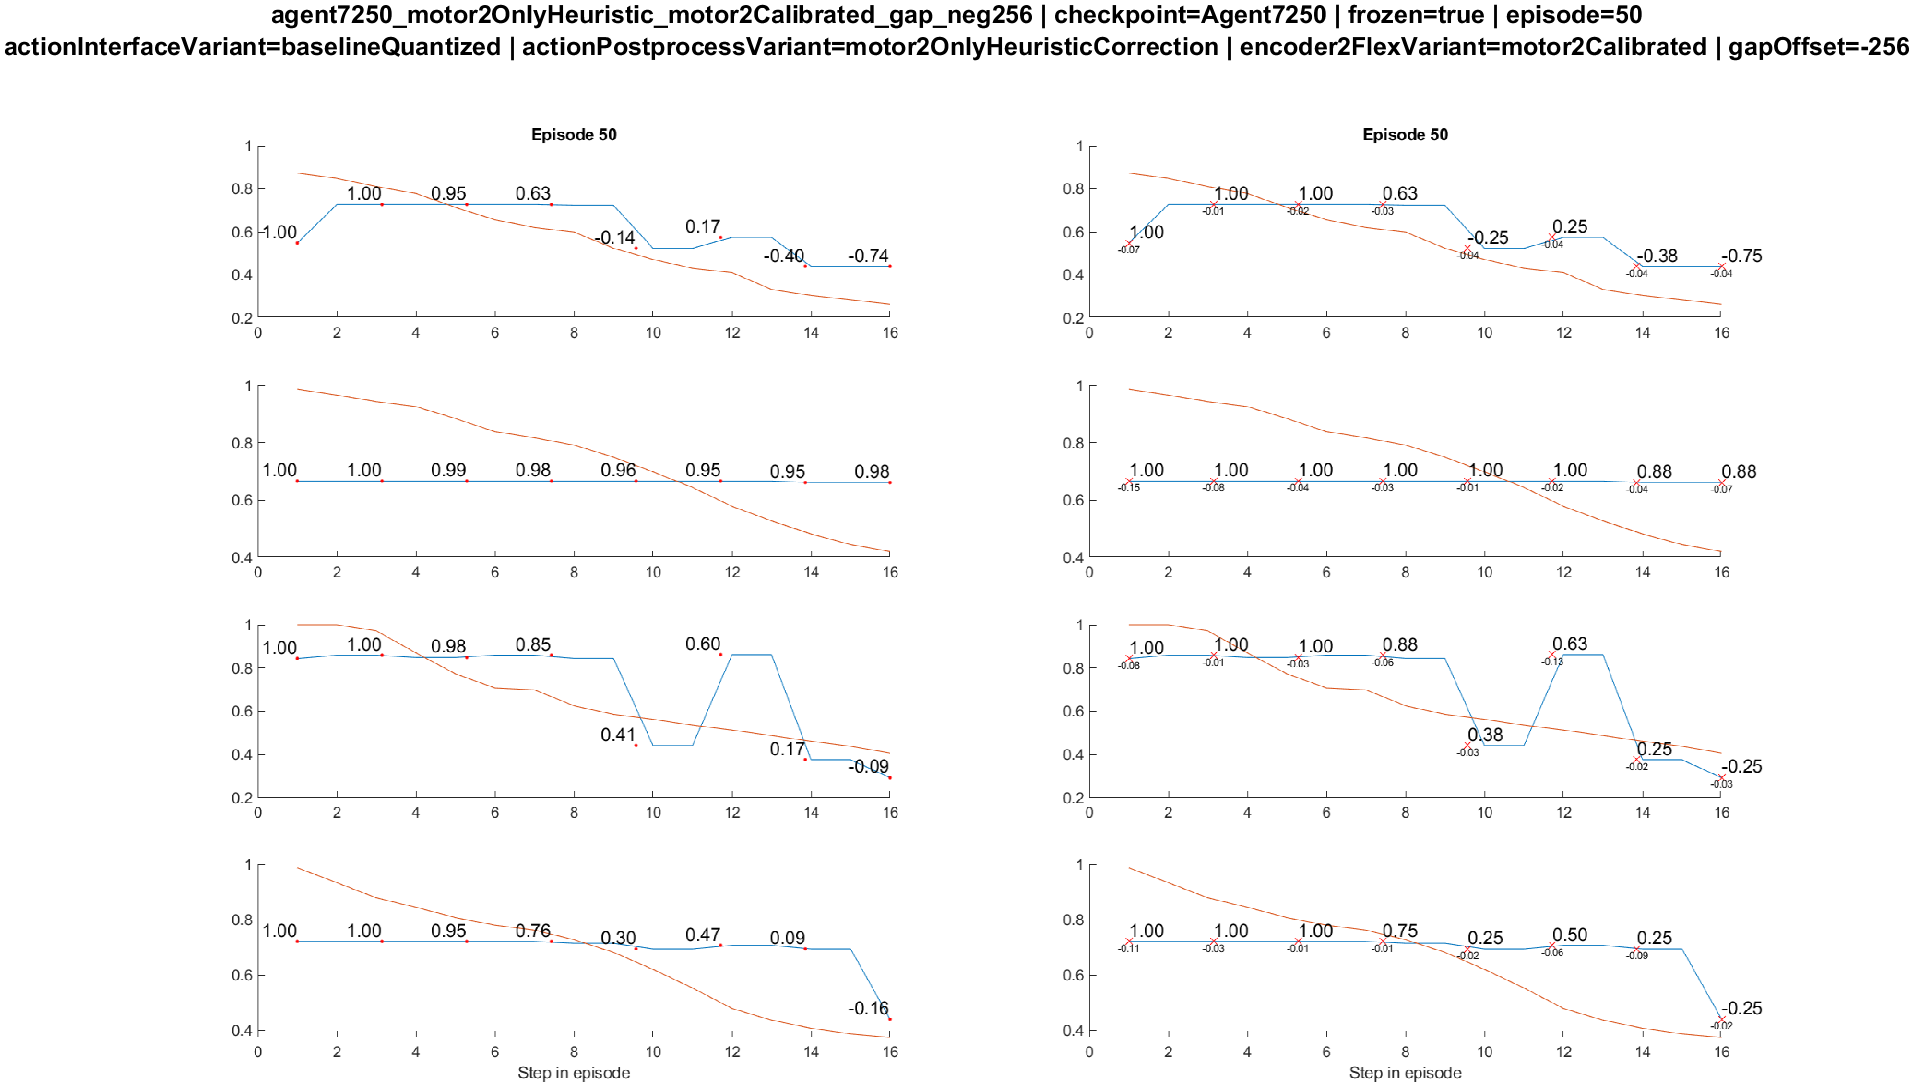
\includegraphics[width=0.92\linewidth]{frozen_agent7250_final/agent7250_m2only_heuristic_motor2Calibrated_gap_neg256_episode50_visual_test_20260623.png}
\caption{Test visual MATLAB, episodio 50, Agent7250 congelado con correccion aislada de motor 2 y conversion calibrada.}
\end{figure}

\section{Evidencia visual de entrenamiento y test}

Las figuras siguientes fueron generadas por MATLAB durante el entrenamiento
y test del checkpoint seleccionado para \texttt{motorCalibratedQuantized}.
Esta variante queda retenida solo como experimento futuro; no se promueve
como linea principal.

\begin{figure}[H]
\centering
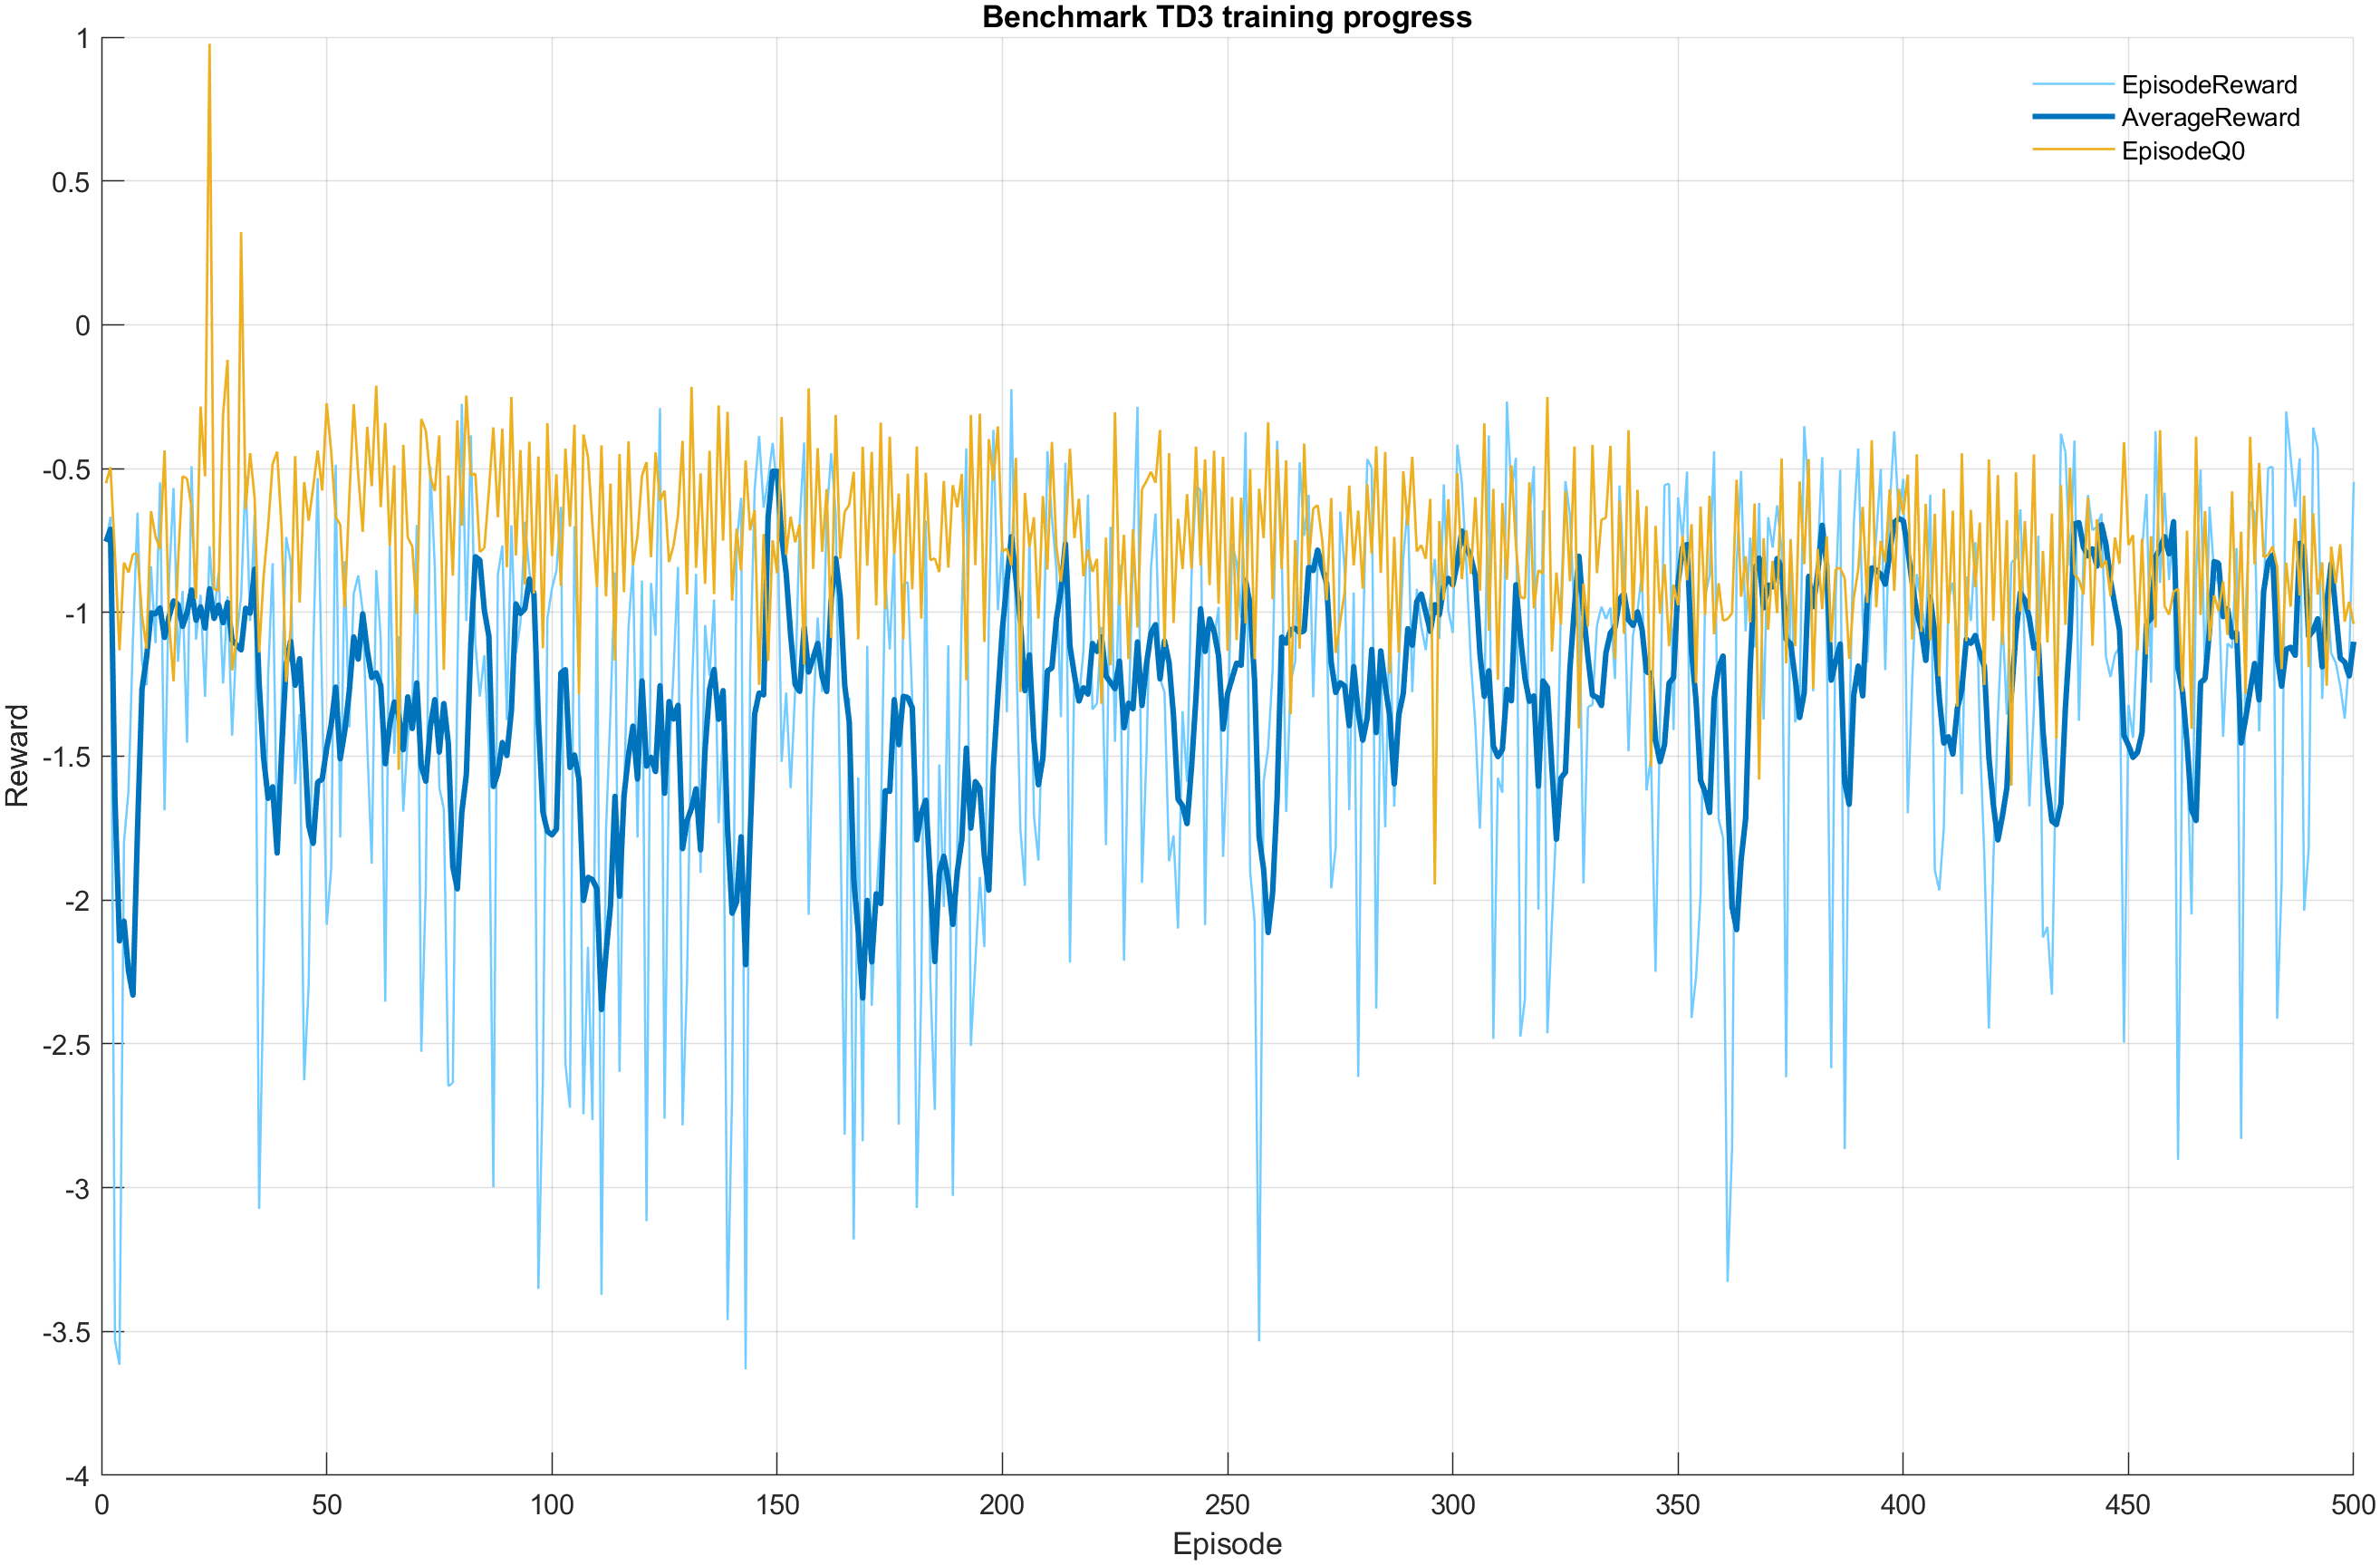
\includegraphics[width=0.92\linewidth]{calibration_motor_calibrated_seed011_training_progress.png}
\caption{Training progress MATLAB, seed 11, accion calibrada.}
\end{figure}

\begin{figure}[H]
\centering
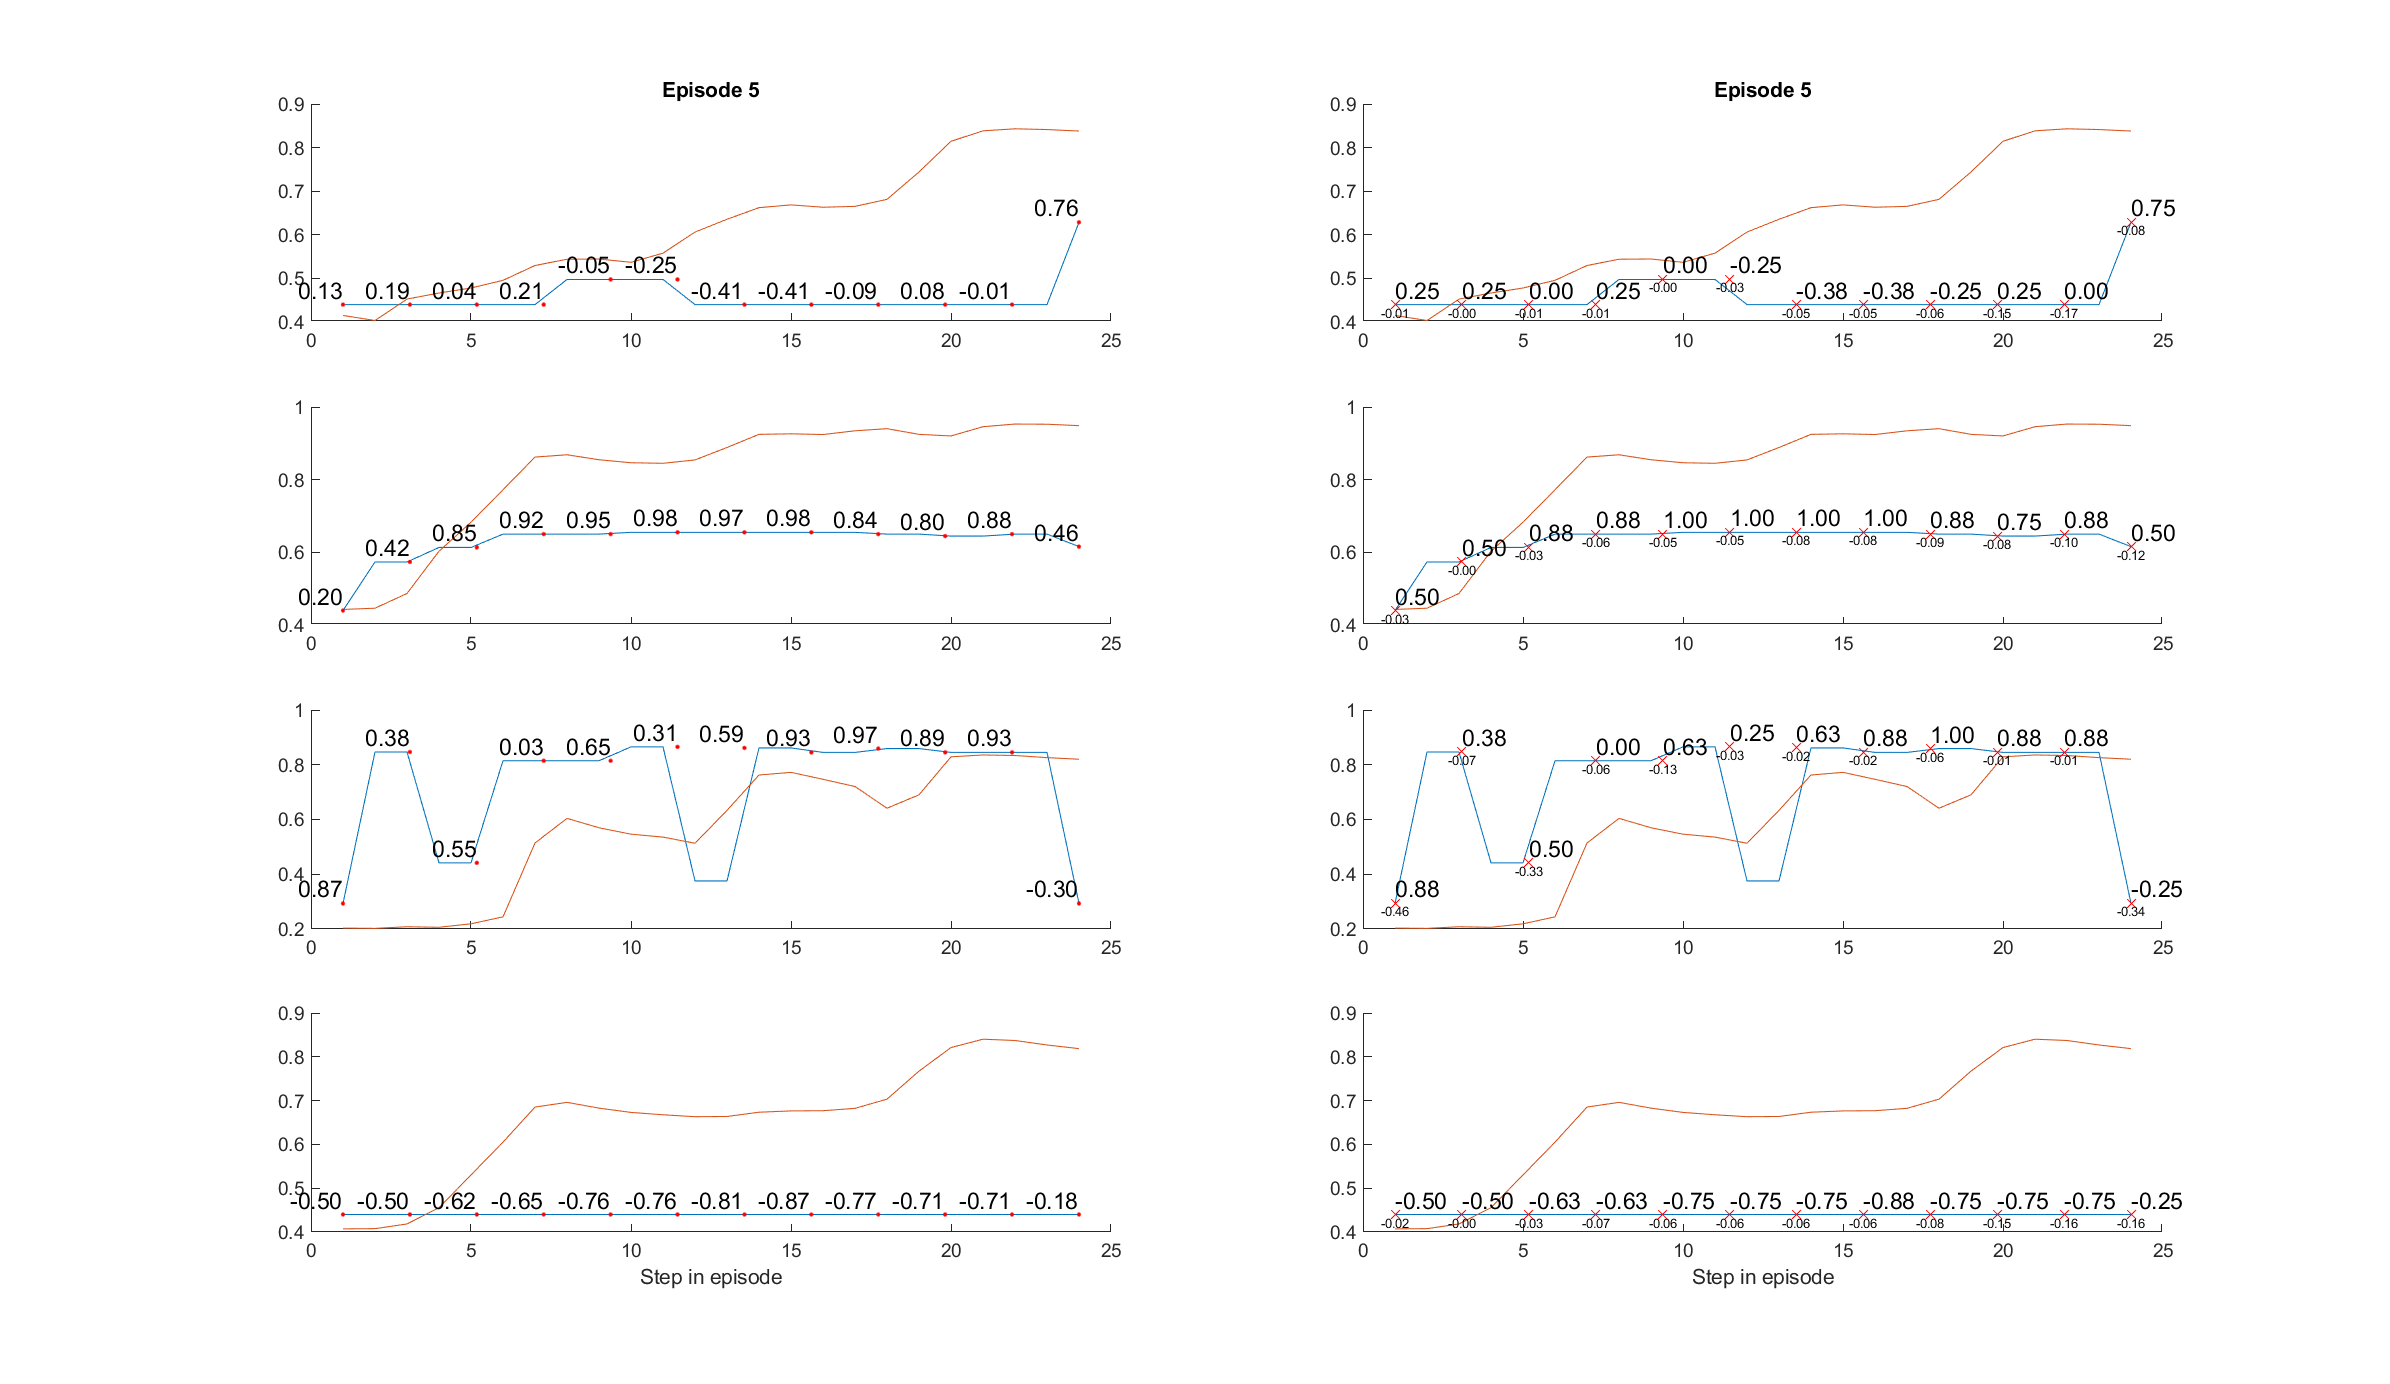
\includegraphics[width=0.92\linewidth]{calibration_motor_calibrated_seed011_visual_test_episode5.png}
\caption{Test visual MATLAB, seed 11, episodio 5, accion calibrada.}
\end{figure}

\section{Auditoria forense de flags de motor 2}

Despues de la evaluacion congelada se hizo una auditoria por episodio para
entender por que motor 2 seguia con flags. No hubo entrenamiento. Se evaluo
\texttt{Agent7250} congelado en cuatro configuraciones: baseline, conversion
\texttt{motor2Calibrated -256}, heuristica M2-only, y heuristica M2-only con
conversion calibrada.

\begin{table}[H]
\centering
\caption{Auditoria forense de flags de motor 2, 50 episodios.}
\scriptsize
\begin{tabular}{lrrrrrrr}
\toprule
Config & Flags M2 & Episodios & Flat & No-motion & High-action & Falsos + & non-M2 \\
\midrule
Baseline & 81 & 27 & 27 & 27 & 27 & 0 & 0 \\
M2Cal -256 & 78 & 26 & 26 & 26 & 26 & 0 & 0 \\
M2 heuristic & 81 & 27 & 27 & 27 & 27 & 0 & 0 \\
M2 heuristic + M2Cal & 78 & 26 & 26 & 26 & 26 & 0 & 0 \\
\bottomrule
\end{tabular}
\end{table}

La conversion calibrada reduce poco el conteo: elimina solo el episodio 49
de la lista de flags y baja de 81 a 78 flags totales. La heuristica M2-only
si cambia la accion de motor 2, pero no toca M1, M3 ni M4:
\texttt{maxNonMotor2ActionDelta=0}. Eso valida la integridad de la correccion
aislada, pero no valida el candidato.

Los flags no parecen falsos positivos con la regla actual. En episodios
marcados, el target de M2 tiene rango claro y la respuesta queda baja. En
baseline, el promedio fue \texttt{targetRange\_M2=0.475309} contra
\texttt{responseRange\_M2=0.019729}. Con heuristica mas conversion calibrada,
fue \texttt{targetRange\_M2=0.469810} contra
\texttt{responseRange\_M2=0.014281}.

Tambien se probo sensibilidad de thresholds. Con reglas relajadas quedan 25
episodios con flags por configuracion. Con regla estricta de respuesta suben
a 40--43 episodios. Por eso no se recomienda aceptar el candidato solo
relajando thresholds.

\begin{figure}[H]
\centering
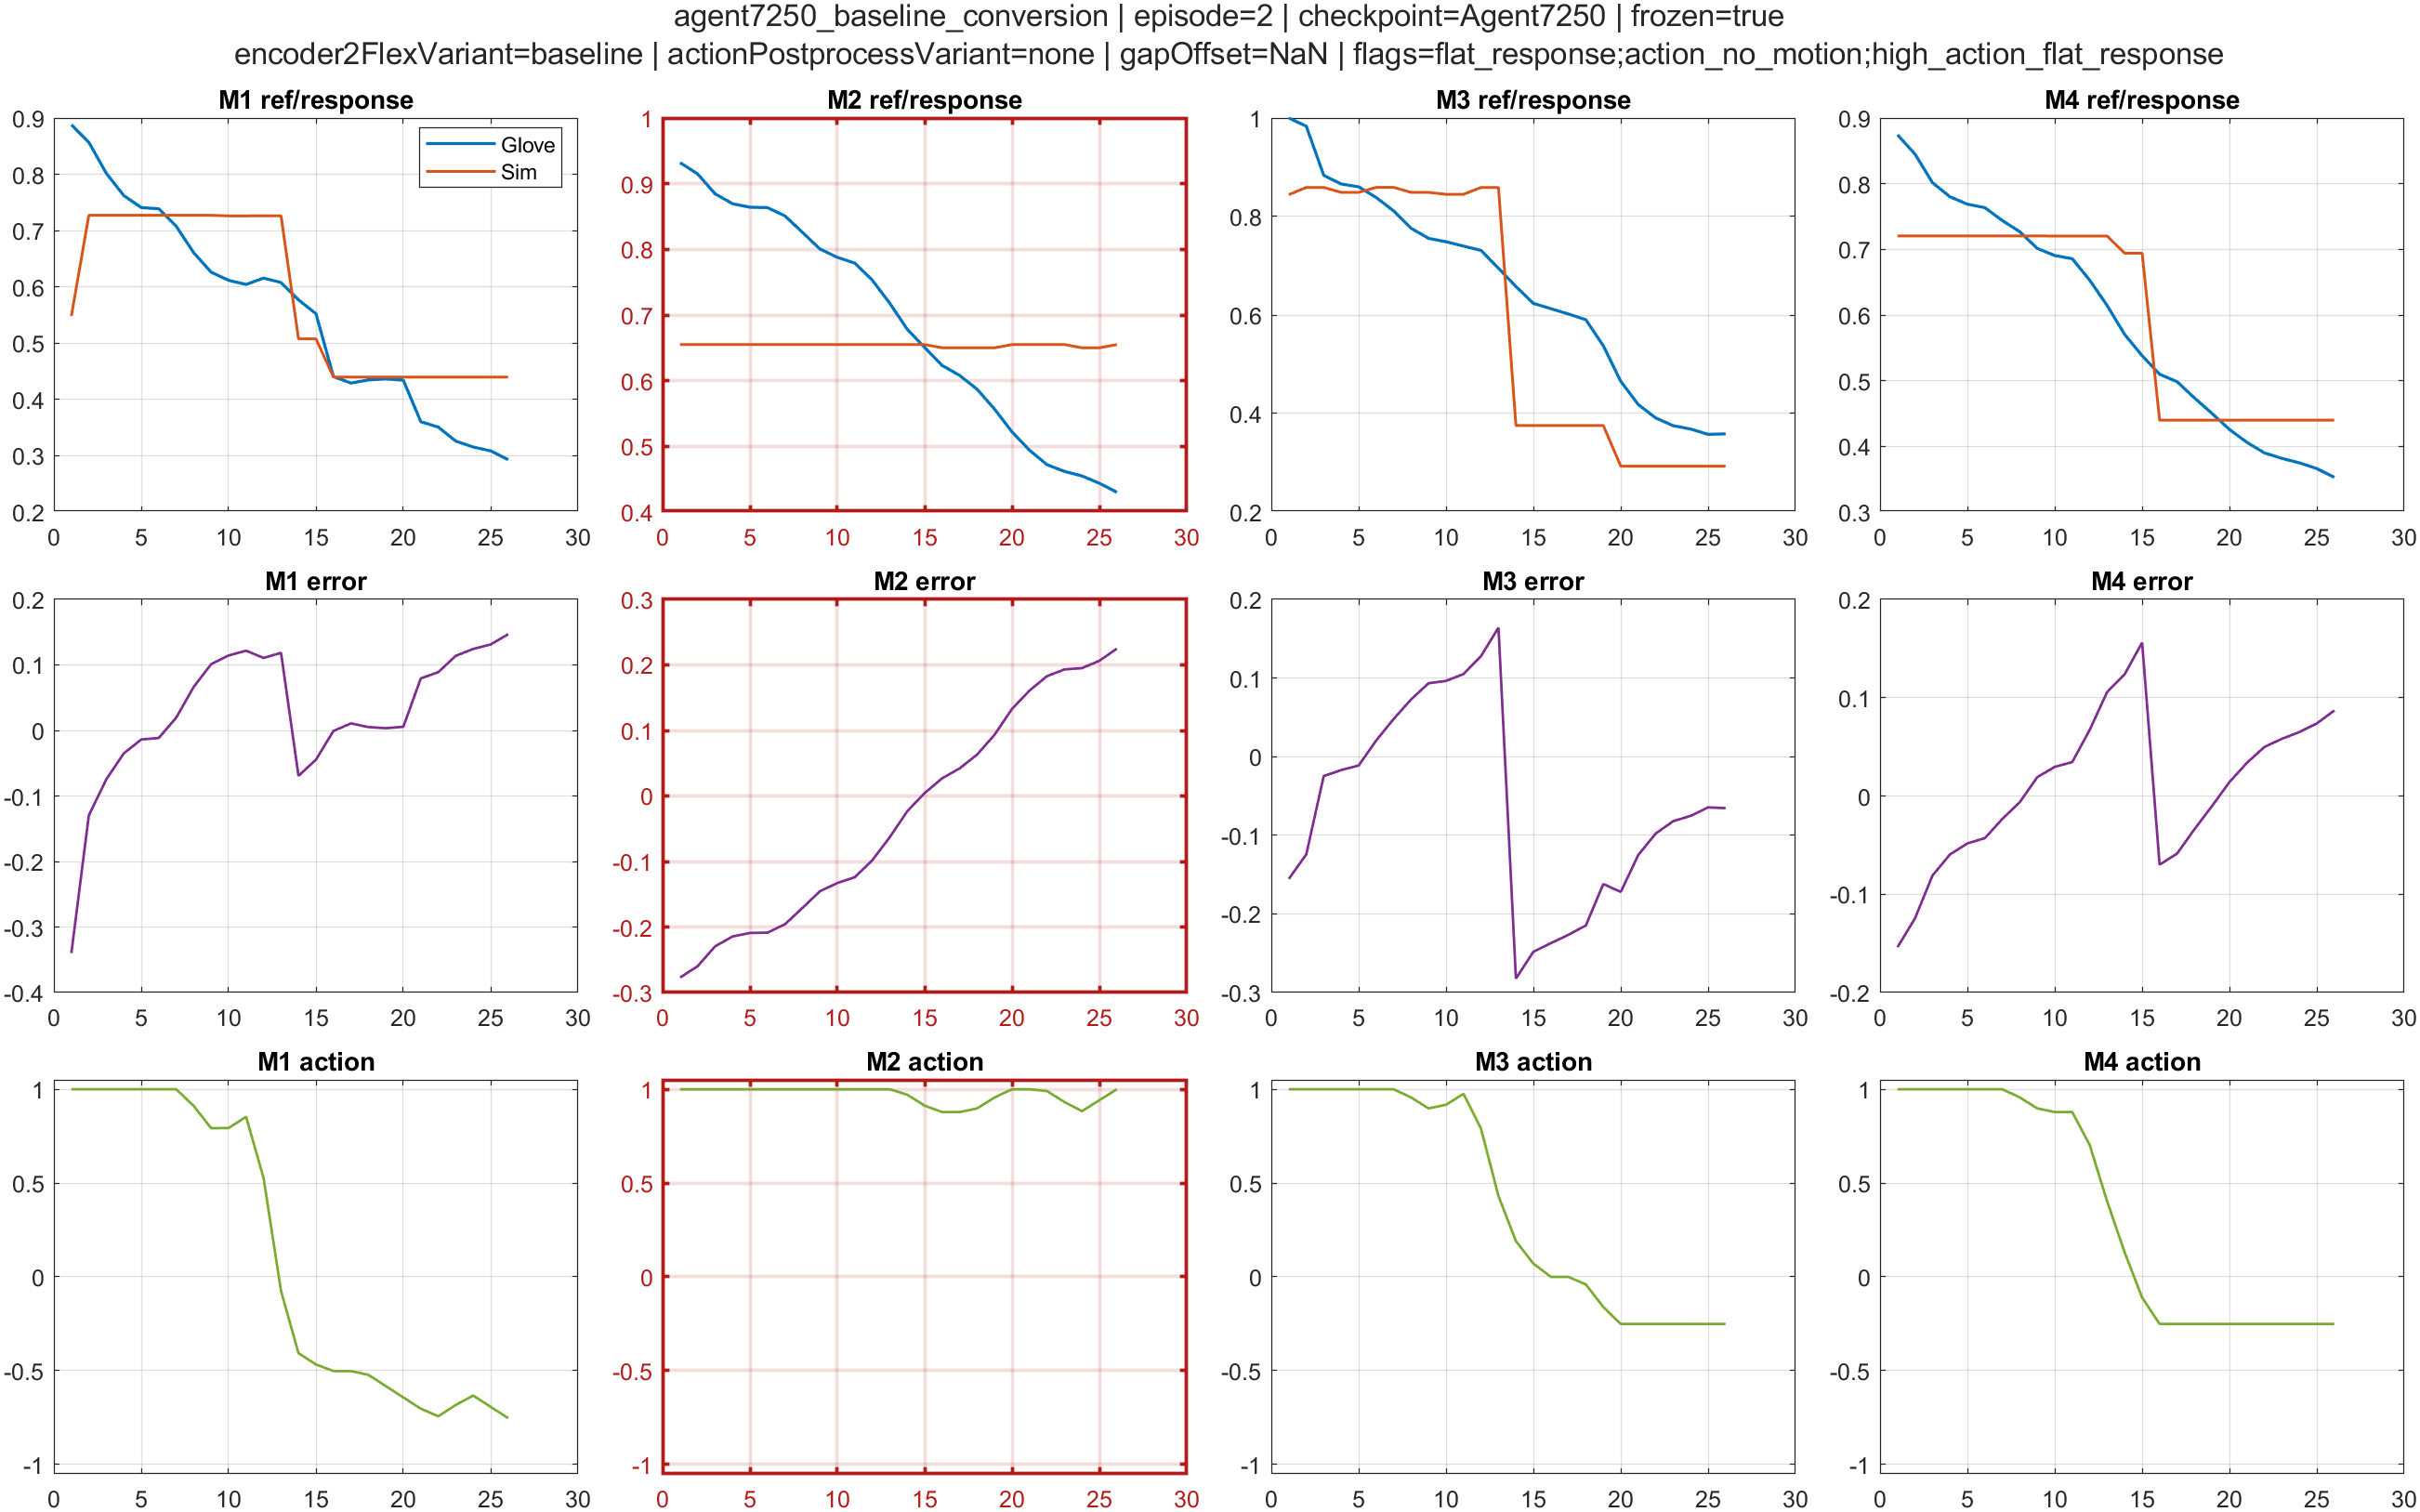
\includegraphics[width=0.92\linewidth]{frozen_agent7250_final/motor2_flag_forensic/a7250_base_episode_002_flags_flat_nomotion_highflat.png}
\caption{Figura MATLAB forense, baseline, episodio 2 con flags de motor 2.}
\end{figure}

\begin{figure}[H]
\centering
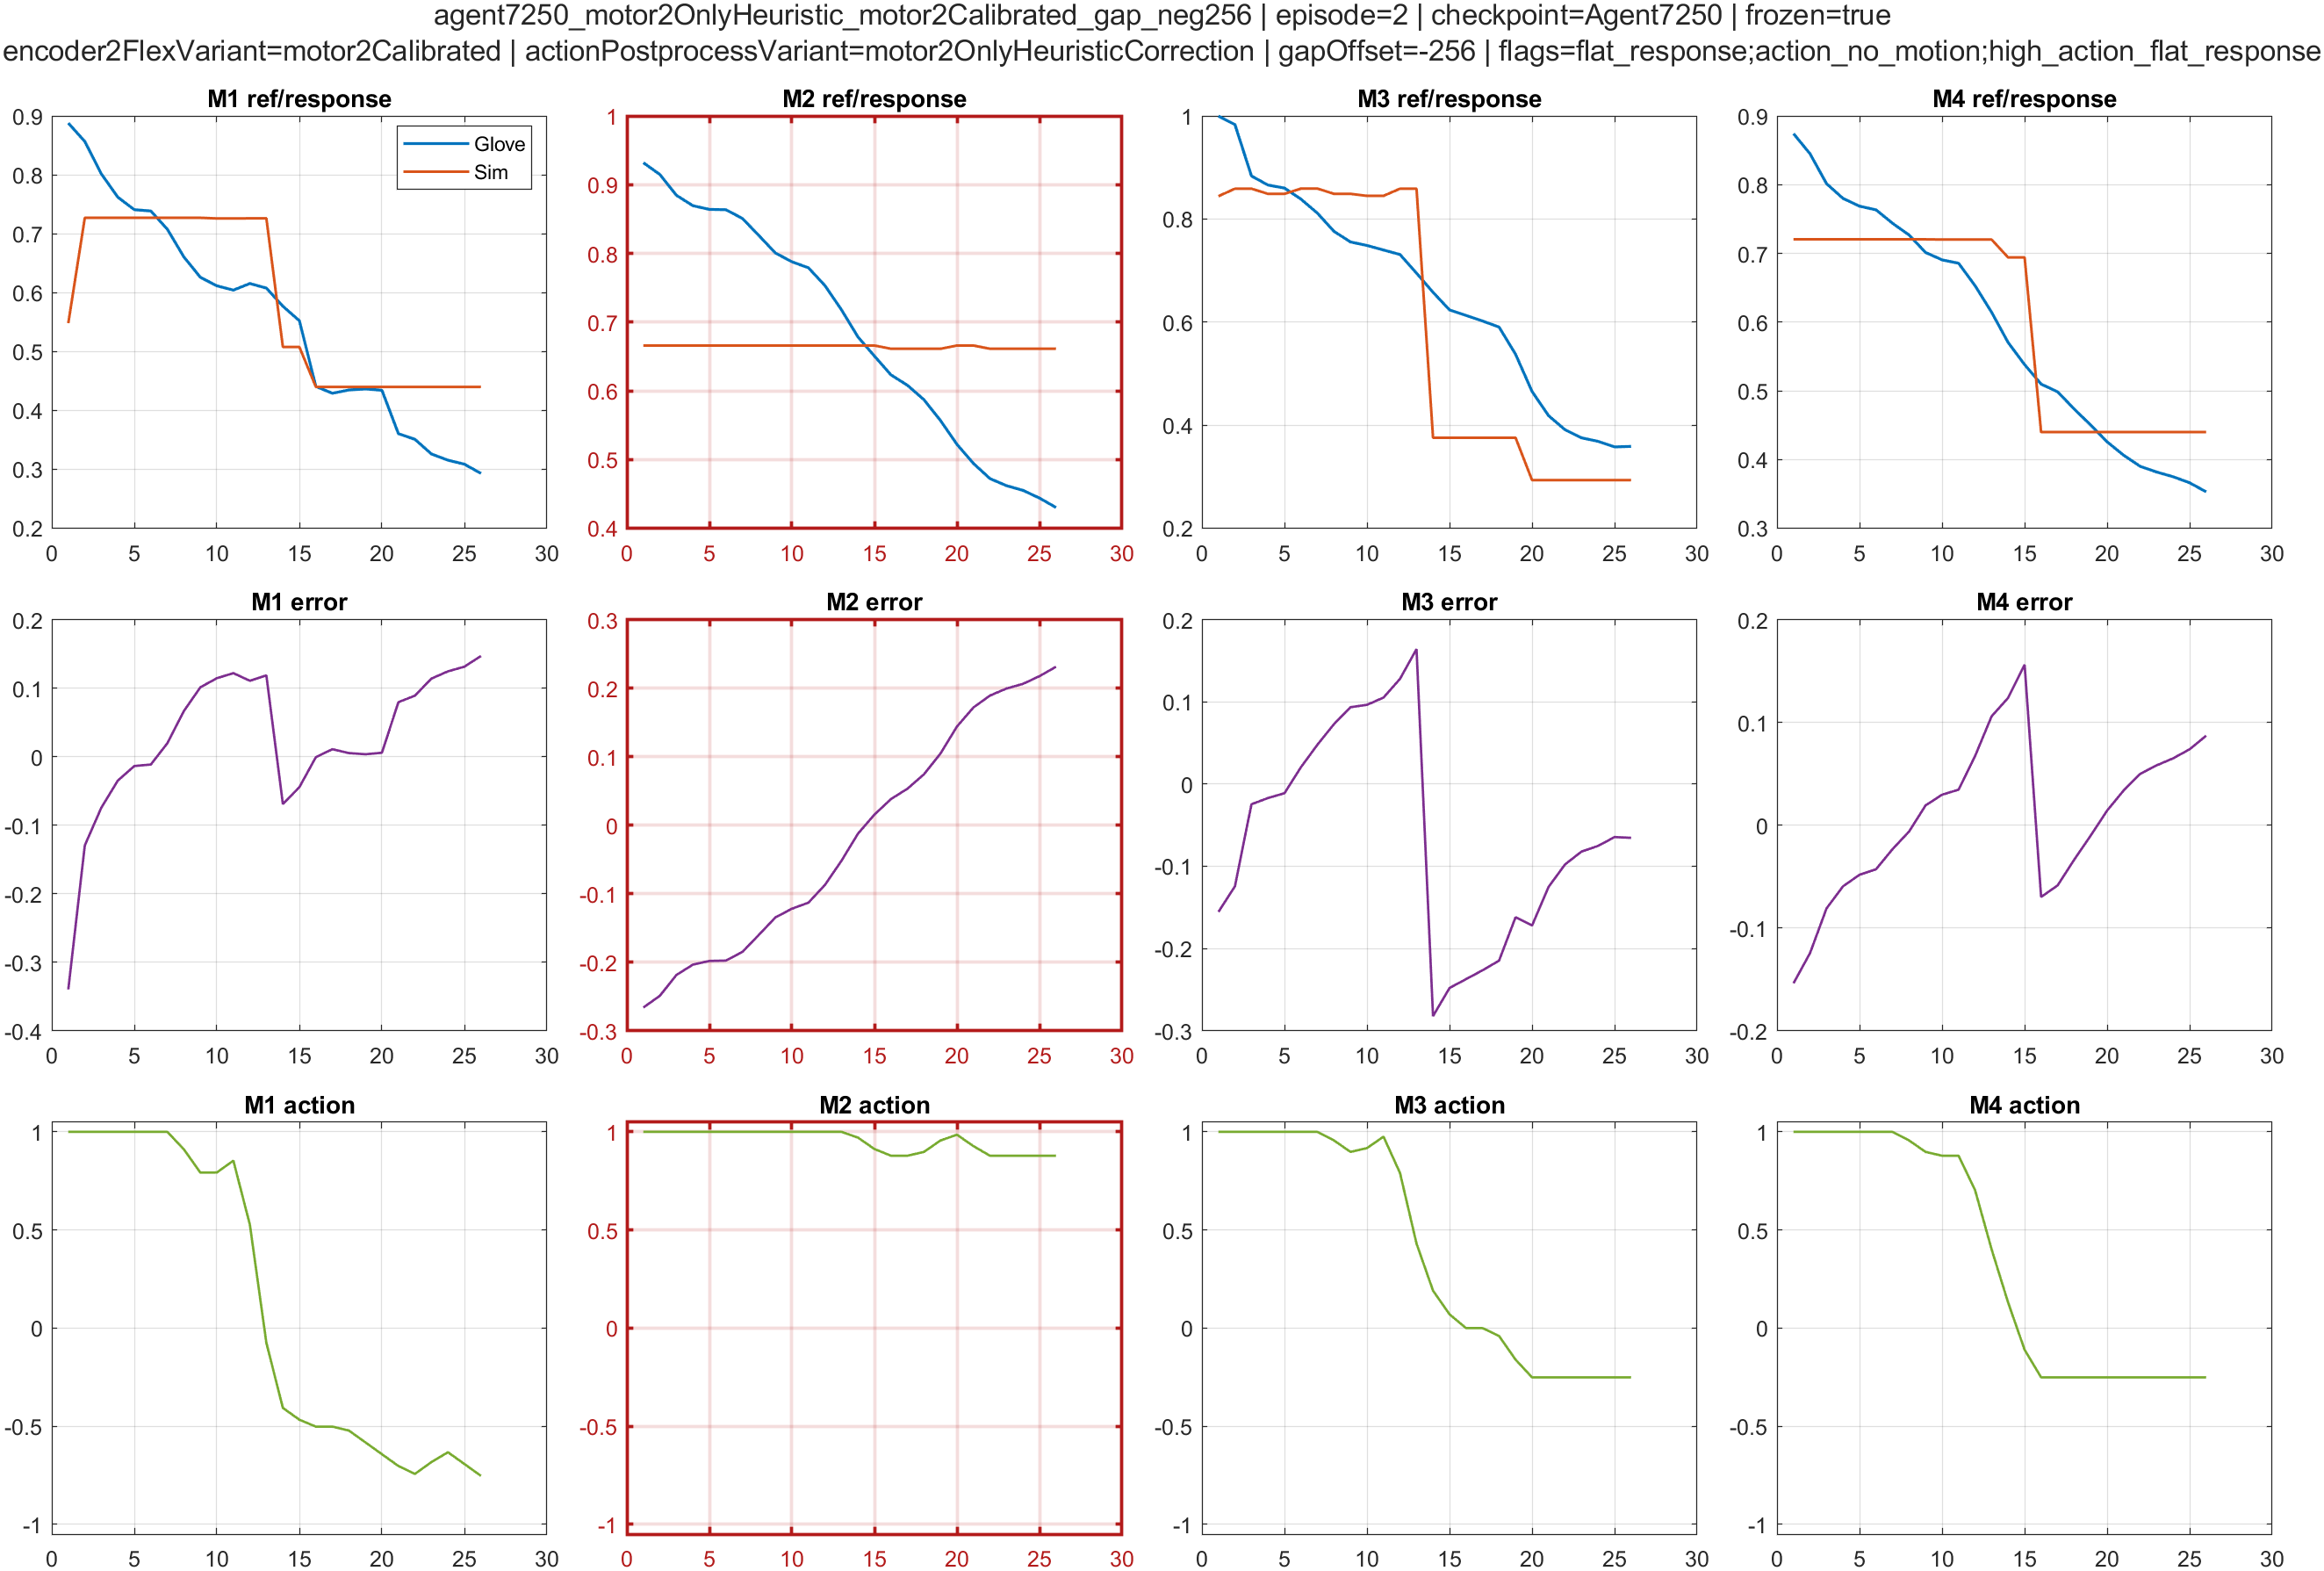
\includegraphics[width=0.92\linewidth]{frozen_agent7250_final/motor2_flag_forensic/a7250_m2heur_m2cal256_episode_002_flags_flat_nomotion_highflat.png}
\caption{Figura MATLAB forense, heuristica M2-only con conversion calibrada, episodio 2 con flags de motor 2.}
\end{figure}

\section{Conclusion}

Se concluye de forma provisional que el problema del motor 2 no es un simple
indice incorrecto. El encoder responde, pero niveles bajos quedan aplanados
en \texttt{encoder2Flex}. La accion calibrada ayuda al error y a la
saturacion, pero no resolvio los flags. La variante experimental
\texttt{motor2Calibrated} con \texttt{gapOffset=-256} paso el smoke corto
cuando se uso junto con \texttt{baselineQuantized}, pero queda rechazada en
la validacion all-motor de 1500 episodios por regresion en M1 y M4. En
cambio, cuando se evaluo sobre \texttt{Agent7250} congelado no degrado M4 y
mejoro levemente motor 2. En la validacion final de 50 episodios, esa mejora
no fue suficiente para aceptarla, porque motor 2 conservo 3 flags.

Antes de volver a reward, Residual Lift o stop-band, conviene revisar
\texttt{gap.idx}, \texttt{breakLimit.idx}, \texttt{encoder2Flex}, la
dinamica del simulador y el comportamiento de motor 4 para posiciones
\texttt{mid} y \texttt{closed}. La direccion actual no es entrenar todo de
nuevo. La direccion actual es usar \texttt{Agent7250} como base congelada y
probar correcciones aisladas de motor 2 que mantengan M1, M3 y M4 intactos.
El candidato actual queda rechazado hasta que limpie los flags de motor 2
sin cambiar acciones de M1, M3 y M4.

La auditoria forense confirma esa decision. La correccion aislada conserva
\texttt{maxNonMotor2ActionDelta=0}, pero M2 mantiene 26--27 episodios con
flags de respuesta plana. La direccion inmediata es explicar esos episodios
marcados y revisar la zona plana de M2 antes de modificar reward, lanzar
campanas largas o retomar residual/stop-band.

\end{document}
